\documentclass[]{book}
\usepackage{lmodern}
\usepackage{amssymb,amsmath}
\usepackage{ifxetex,ifluatex}
\usepackage{fixltx2e} % provides \textsubscript
\ifnum 0\ifxetex 1\fi\ifluatex 1\fi=0 % if pdftex
  \usepackage[T1]{fontenc}
  \usepackage[utf8]{inputenc}
\else % if luatex or xelatex
  \ifxetex
    \usepackage{mathspec}
  \else
    \usepackage{fontspec}
  \fi
  \defaultfontfeatures{Ligatures=TeX,Scale=MatchLowercase}
\fi
% use upquote if available, for straight quotes in verbatim environments
\IfFileExists{upquote.sty}{\usepackage{upquote}}{}
% use microtype if available
\IfFileExists{microtype.sty}{%
\usepackage{microtype}
\UseMicrotypeSet[protrusion]{basicmath} % disable protrusion for tt fonts
}{}
\usepackage[margin=1in]{geometry}
\usepackage{hyperref}
\hypersetup{unicode=true,
            pdftitle={Using Spatial Data with R},
            pdfauthor={Claudia A Engel},
            pdfborder={0 0 0},
            breaklinks=true}
\urlstyle{same}  % don't use monospace font for urls
\usepackage{natbib}
\bibliographystyle{apalike}
\usepackage{color}
\usepackage{fancyvrb}
\newcommand{\VerbBar}{|}
\newcommand{\VERB}{\Verb[commandchars=\\\{\}]}
\DefineVerbatimEnvironment{Highlighting}{Verbatim}{commandchars=\\\{\}}
% Add ',fontsize=\small' for more characters per line
\usepackage{framed}
\definecolor{shadecolor}{RGB}{248,248,248}
\newenvironment{Shaded}{\begin{snugshade}}{\end{snugshade}}
\newcommand{\KeywordTok}[1]{\textcolor[rgb]{0.13,0.29,0.53}{\textbf{#1}}}
\newcommand{\DataTypeTok}[1]{\textcolor[rgb]{0.13,0.29,0.53}{#1}}
\newcommand{\DecValTok}[1]{\textcolor[rgb]{0.00,0.00,0.81}{#1}}
\newcommand{\BaseNTok}[1]{\textcolor[rgb]{0.00,0.00,0.81}{#1}}
\newcommand{\FloatTok}[1]{\textcolor[rgb]{0.00,0.00,0.81}{#1}}
\newcommand{\ConstantTok}[1]{\textcolor[rgb]{0.00,0.00,0.00}{#1}}
\newcommand{\CharTok}[1]{\textcolor[rgb]{0.31,0.60,0.02}{#1}}
\newcommand{\SpecialCharTok}[1]{\textcolor[rgb]{0.00,0.00,0.00}{#1}}
\newcommand{\StringTok}[1]{\textcolor[rgb]{0.31,0.60,0.02}{#1}}
\newcommand{\VerbatimStringTok}[1]{\textcolor[rgb]{0.31,0.60,0.02}{#1}}
\newcommand{\SpecialStringTok}[1]{\textcolor[rgb]{0.31,0.60,0.02}{#1}}
\newcommand{\ImportTok}[1]{#1}
\newcommand{\CommentTok}[1]{\textcolor[rgb]{0.56,0.35,0.01}{\textit{#1}}}
\newcommand{\DocumentationTok}[1]{\textcolor[rgb]{0.56,0.35,0.01}{\textbf{\textit{#1}}}}
\newcommand{\AnnotationTok}[1]{\textcolor[rgb]{0.56,0.35,0.01}{\textbf{\textit{#1}}}}
\newcommand{\CommentVarTok}[1]{\textcolor[rgb]{0.56,0.35,0.01}{\textbf{\textit{#1}}}}
\newcommand{\OtherTok}[1]{\textcolor[rgb]{0.56,0.35,0.01}{#1}}
\newcommand{\FunctionTok}[1]{\textcolor[rgb]{0.00,0.00,0.00}{#1}}
\newcommand{\VariableTok}[1]{\textcolor[rgb]{0.00,0.00,0.00}{#1}}
\newcommand{\ControlFlowTok}[1]{\textcolor[rgb]{0.13,0.29,0.53}{\textbf{#1}}}
\newcommand{\OperatorTok}[1]{\textcolor[rgb]{0.81,0.36,0.00}{\textbf{#1}}}
\newcommand{\BuiltInTok}[1]{#1}
\newcommand{\ExtensionTok}[1]{#1}
\newcommand{\PreprocessorTok}[1]{\textcolor[rgb]{0.56,0.35,0.01}{\textit{#1}}}
\newcommand{\AttributeTok}[1]{\textcolor[rgb]{0.77,0.63,0.00}{#1}}
\newcommand{\RegionMarkerTok}[1]{#1}
\newcommand{\InformationTok}[1]{\textcolor[rgb]{0.56,0.35,0.01}{\textbf{\textit{#1}}}}
\newcommand{\WarningTok}[1]{\textcolor[rgb]{0.56,0.35,0.01}{\textbf{\textit{#1}}}}
\newcommand{\AlertTok}[1]{\textcolor[rgb]{0.94,0.16,0.16}{#1}}
\newcommand{\ErrorTok}[1]{\textcolor[rgb]{0.64,0.00,0.00}{\textbf{#1}}}
\newcommand{\NormalTok}[1]{#1}
\usepackage{longtable,booktabs}
\usepackage{graphicx,grffile}
\makeatletter
\def\maxwidth{\ifdim\Gin@nat@width>\linewidth\linewidth\else\Gin@nat@width\fi}
\def\maxheight{\ifdim\Gin@nat@height>\textheight\textheight\else\Gin@nat@height\fi}
\makeatother
% Scale images if necessary, so that they will not overflow the page
% margins by default, and it is still possible to overwrite the defaults
% using explicit options in \includegraphics[width, height, ...]{}
\setkeys{Gin}{width=\maxwidth,height=\maxheight,keepaspectratio}
\IfFileExists{parskip.sty}{%
\usepackage{parskip}
}{% else
\setlength{\parindent}{0pt}
\setlength{\parskip}{6pt plus 2pt minus 1pt}
}
\setlength{\emergencystretch}{3em}  % prevent overfull lines
\providecommand{\tightlist}{%
  \setlength{\itemsep}{0pt}\setlength{\parskip}{0pt}}
\setcounter{secnumdepth}{5}
% Redefines (sub)paragraphs to behave more like sections
\ifx\paragraph\undefined\else
\let\oldparagraph\paragraph
\renewcommand{\paragraph}[1]{\oldparagraph{#1}\mbox{}}
\fi
\ifx\subparagraph\undefined\else
\let\oldsubparagraph\subparagraph
\renewcommand{\subparagraph}[1]{\oldsubparagraph{#1}\mbox{}}
\fi

%%% Use protect on footnotes to avoid problems with footnotes in titles
\let\rmarkdownfootnote\footnote%
\def\footnote{\protect\rmarkdownfootnote}

%%% Change title format to be more compact
\usepackage{titling}

% Create subtitle command for use in maketitle
\newcommand{\subtitle}[1]{
  \posttitle{
    \begin{center}\large#1\end{center}
    }
}

\setlength{\droptitle}{-2em}

  \title{Using Spatial Data with R}
    \pretitle{\vspace{\droptitle}\centering\huge}
  \posttitle{\par}
    \author{Claudia A Engel}
    \preauthor{\centering\large\emph}
  \postauthor{\par}
      \predate{\centering\large\emph}
  \postdate{\par}
    \date{Last updated: February 11, 2019}

\usepackage{booktabs}
\usepackage{amsthm}
\makeatletter
\def\thm@space@setup{%
  \thm@preskip=8pt plus 2pt minus 4pt
  \thm@postskip=\thm@preskip
}
\makeatother

\begin{document}
\maketitle

{
\setcounter{tocdepth}{1}
\tableofcontents
}
\chapter*{Prerequisites and
Preparations}\label{prerequisites-and-preparations}
\addcontentsline{toc}{chapter}{Prerequisites and Preparations}

To get the most out of this workshop you should have:

\begin{itemize}
\tightlist
\item
  a \textbf{basic knowledge} of R and/or be familiar with the topics
  covered in the \href{https://cengel.github.io/R-intro/}{Introduction
  to R}.
\item
  have a recent version of \href{https://cran.r-project.org/}{R} and
  \href{https://www.rstudio.com/}{RStudio} installed.
\end{itemize}

\textbf{Recommended}:

\begin{itemize}
\item
  Create a new RStudio project \texttt{R-spatial} in a new folder
  \texttt{R-spatial}.
\item
  Create a new folder under \texttt{R-spatial} and call it
  \texttt{data}.
\item
  If you have your working directory set to \texttt{R-spatial} which
  contains a folder called \texttt{data} you can copy, paste, and run
  the following lines in R:
\end{itemize}

\begin{Shaded}
\begin{Highlighting}[]
\KeywordTok{download.file}\NormalTok{(}\StringTok{"http://bit.ly/R-spatial-data"}\NormalTok{, }\StringTok{"R-spatial-data.zip"}\NormalTok{)}
\KeywordTok{unzip}\NormalTok{(}\StringTok{"R-spatial-data.zip"}\NormalTok{, }\DataTypeTok{exdir =} \StringTok{"data"}\NormalTok{)}
\end{Highlighting}
\end{Shaded}

You can also download the data manually here
\href{https://github.com/cengel/R-spatial/raw/master/data/R-spatial-data.zip}{R-spatial-data.zip}
and extract them.

\begin{itemize}
\item
  Open up a new R Script file \texttt{R-spatial.R} for the code you'll
  create during the workshop.
\item
  Install and load the following libraries:

  \begin{itemize}
  \tightlist
  \item
    \href{https://cran.r-project.org/package=sf}{\texttt{sf}}
  \item
    \href{https://CRAN.R-project.org/package=sp}{\texttt{sp}}
  \item
    \href{https://CRAN.R-project.org/package=rgdal}{\texttt{rgdal}}
  \item
    \href{https://CRAN.R-project.org/package=raster}{\texttt{raster}}
  \item
    \href{https://CRAN.R-project.org/package=rgeos}{\texttt{rgeos}}
  \item
    \href{https://cran.r-project.org/package=dplyr}{\texttt{dplyr}}
  \end{itemize}
\item
  For the mapping section install and load these additional libraries:

  \begin{itemize}
  \tightlist
  \item
    \href{https://cran.r-project.org/package=classInt}{\texttt{classInt}}
  \item
    \href{https://cran.r-project.org/package=RColorBrewer}{\texttt{RColorBrewer}}
  \item
    \href{https://cran.r-project.org/package=ggplot2}{\texttt{ggplot2}}
  \item
    \href{https://cran.r-project.org/package=ggmap}{\texttt{ggmap}}
  \item
    \href{https://cran.r-project.org/package=tmap}{\texttt{tmap}}
  \item
    \href{https://cran.r-project.org/package=leaflet}{\texttt{leaflet}}(On
    Mac installing binary version is ok)
  \end{itemize}
\end{itemize}

\section*{References}\label{references}
\addcontentsline{toc}{section}{References}

Bivand, RS., Pebesma, E., Gómez-Rubio, V. (2013):
\href{https://link.springer.com/book/10.1007\%2F978-1-4614-7618-4}{Applied
Spatial Data Analysis with R}

Brunsdon, C. and Comber, L. (2015):
\href{https://us.sagepub.com/en-us/nam/an-introduction-to-r-for-spatial-analysis-and-mapping/book241031}{An
Introduction to R for Spatial Analysis and Mapping}

Lovelace, R., Nowosad, J., Muenchow. J. (2019):
\href{https://geocompr.robinlovelace.net}{Geocomputation with R}

\href{http://www.rspatial.org/index.html}{Spatial Data Analysis and
Modeling with R}

\href{https://CRAN.R-project.org/view=Spatial}{CRAN Task View: Analysis
of Spatial Data}

Engel, C. (2019). R for Geospatial Analysis and Mapping. The Geographic
Information Science \& Technology Body of Knowledge (1st Quarter 2019
Edition), John P. Wilson (Ed.).
\href{https://doi.org/10.22224/gistbok/2019.1.3}{DOI:10.22224/gistbok/2019.1.3}.

For a quick introduction to all things geo check out
\href{https://mapschool.io}{map school}.

\section*{Acknowledgements}\label{acknowledgements}
\addcontentsline{toc}{section}{Acknowledgements}

Some of the materials for this tutorial are adapted from
\url{http://datacarpentry.org}

\chapter{Introduction to spatial data in R}\label{intro}

\begin{quote}
Learning Objectives

\begin{itemize}
\tightlist
\item
  Create point, line, and polygon shapefiles as \texttt{sp} and
  \texttt{sf} objects.
\item
  Read shapefiles into \texttt{sp} and \texttt{sf} objects
\item
  Examine \texttt{sp} and \texttt{sf} objects
\item
  Read GeoTiff single and multiband into a \texttt{raster} object.
\item
  Examine \texttt{raster} objects
\end{itemize}
\end{quote}

\begin{center}\rule{0.5\linewidth}{\linethickness}\end{center}

\section{Conceptualizing spatial vector objects in
R}\label{conceptualizing-spatial-vector-objects-in-r}

In vector GIS we deal with, points, lines, and polygons, like so:

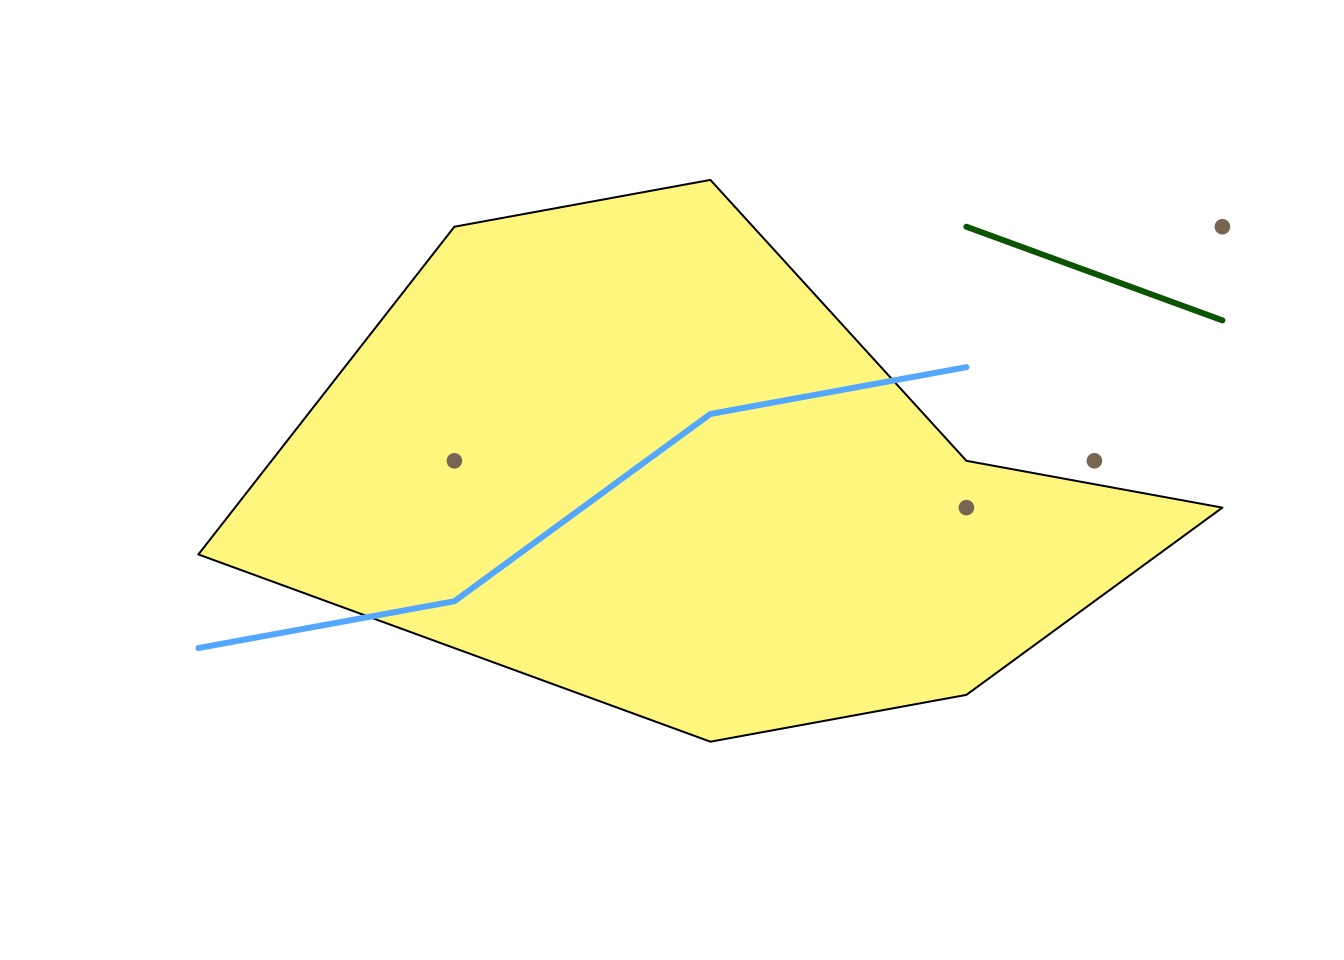
\includegraphics{R-spatial_files/figure-latex/unnamed-chunk-2-1.pdf}

\begin{quote}
Challenge

Discuss with your neighbor: What information do we need to store in
order to define points, lines, polygons in geographic space?
\end{quote}

There are currently two main approaches in R to handle geographic vector
data:

\subsection{\texorpdfstring{The \texttt{sp}
package}{The sp package}}\label{the-sp-package}

The first general package to provide classes and methods for spatial
data types that was developed for R is called
\href{https://cran.r-project.org/package=sp}{\texttt{sp}}\footnote{R
  Bivand (2011)
  \href{http://geostat-course.org/system/files/monday_slides.pdf}{Introduction
  to representing spatial objects in R}}. Development of the \texttt{sp}
package began in the early 2000s in an attempt to standardize how
spatial data would be treated in R and to allow for better
interoperability between different analysis packages that use spatial
data. The package (first release on CRAN in 2005) provides classes and
methods to create \emph{points}, \emph{lines}, \emph{polygons}, and
\emph{grids} and to operate on them. About 350 of the spatial analysis
packages use the spatial data types that are implemented in \texttt{sp}
i.e.~they ``depend'' on the \texttt{sp} package and many more are
indirectly dependent.

The foundational structure for any spatial object in \texttt{sp} is the
\texttt{Spatial} class. It has two ``slots''
(\href{http://stackoverflow.com/a/4714080}{new-style S4 class objects in
R have pre-defined components called slots}):

\begin{itemize}
\item
  a \textbf{bounding box}
\item
  a \textbf{CRS class object} to define the Coordinate Reference System
\end{itemize}

This basic structure is then extended, depending on the characteristics
of the spatial object (point, line, polygon).

To manually build up a spatial object in \texttt{sp} we could follow
these steps:

\begin{quote}
\textbf{I. Create geometric objects (topology)}
\end{quote}

\textbf{Points} (which may have 2 or 3 dimensions) are the most basic
spatial data objects. They are generated out of either a single
coordinate or a set of coordinates, like a two-column matrix or a
dataframe with a column for latitude and one for longitude.\\
\textbf{Lines} are generated out of \texttt{Line} objects. A
\texttt{Line} object is a spaghetti collection of 2D
coordinates\footnote{Coordinates should be of type double and will be
  promoted if not.} and is generated out of a two-column matrix or a
dataframe with a column for latitude and one for longitude. A
\texttt{Lines} object is a \textbf{list} of one or more \texttt{Line}
objects, for example all the contours at a single elevation.\\
\textbf{Polygons} are generated out of \texttt{Polygon} objects. A
\texttt{Polygon} object is a spaghetti collection of 2D coordinates with
equal first and last coordinates and is generated out of a two-column
matrix or a dataframe with a column for latitude and one for longitude.
A \texttt{Polygons} object is a \textbf{list} of one or more
\texttt{Polygon} objects, for example islands belonging to the same
country.

\begin{quote}
\textbf{II. Create spatial objects \texttt{Spatial*} object (\texttt{*}
stands for Points, Lines, or Polygons).}
\end{quote}

This step adds the bounding box (automatically) and the slot for the
Coordinate Reference System or CRS (which needs to be filled with a
value manually). \texttt{SpatialPoints} can be directly generated out of
the coordinates. \texttt{SpatialLines} and \texttt{SpatialPolygons}
objects are generated using lists of \texttt{Lines} or \texttt{Polygons}
objects respectively (more below).

\begin{quote}
\textbf{III. Add attributes (\emph{Optional}:)}
\end{quote}

Add a data frame with attribute data, which will turn your
\texttt{Spatial*} object into a \texttt{Spatial*DataFrame} object. The
points in a \texttt{SpatialPoints} object may be associated with a row
of attributes to create a \texttt{SpatialPointsDataFrame} object. The
coordinates and attributes may, but do not have to be keyed to each
other using ID values.\\
\texttt{SpatialLinesDataFrame} and \texttt{SpatialPolygonsDataFrame}
objects are defined using \texttt{SpatialLines} and
\texttt{SpatialPolygons} objects and data frames. The ID fields are here
required to match the data frame row names.

If, for example we wanted to build up an \texttt{sp} Object that would
contain highways we would do the following.

First we would create a \texttt{Line} object that holds one highway. We
use a matrix with two columns of arbitrary numbers, for x and y
coordinates.

\begin{Shaded}
\begin{Highlighting}[]
\NormalTok{ln1 <-}\StringTok{ }\KeywordTok{Line}\NormalTok{(}\KeywordTok{matrix}\NormalTok{(}\KeywordTok{runif}\NormalTok{(}\DecValTok{6}\NormalTok{), }\DataTypeTok{ncol=}\DecValTok{2}\NormalTok{))}
\KeywordTok{str}\NormalTok{(ln1)}
\end{Highlighting}
\end{Shaded}

\begin{verbatim}
#> Formal class 'Line' [package "sp"] with 1 slot
#>   ..@ coords: num [1:3, 1:2] 0.449 0.94 0.249 0.435 0.208 ...
\end{verbatim}

Note the \texttt{@\ coords} slot which holds the coordinates.

Ok, let's create another \texttt{Line} object for another highway:

\begin{Shaded}
\begin{Highlighting}[]
\NormalTok{ln2 <-}\StringTok{ }\KeywordTok{Line}\NormalTok{(}\KeywordTok{matrix}\NormalTok{(}\KeywordTok{runif}\NormalTok{(}\DecValTok{6}\NormalTok{), }\DataTypeTok{ncol=}\DecValTok{2}\NormalTok{))}
\end{Highlighting}
\end{Shaded}

Now we combine the two highways to a \texttt{Lines} object. Note how we
add a unique ID for each highway. This step allows to combine generate
multiple line strings, so we could add more lines under the same ID.

\begin{Shaded}
\begin{Highlighting}[]
\NormalTok{lns1 <-}\StringTok{ }\KeywordTok{Lines}\NormalTok{(}\KeywordTok{list}\NormalTok{(ln1), }\DataTypeTok{ID =} \KeywordTok{c}\NormalTok{(}\StringTok{"hwy1"}\NormalTok{)) }
\NormalTok{lns2 <-}\StringTok{ }\KeywordTok{Lines}\NormalTok{(}\KeywordTok{list}\NormalTok{(ln2), }\DataTypeTok{ID =} \KeywordTok{c}\NormalTok{(}\StringTok{"hwy2"}\NormalTok{)) }
\KeywordTok{str}\NormalTok{(lns1)}
\end{Highlighting}
\end{Shaded}

\begin{verbatim}
#> Formal class 'Lines' [package "sp"] with 2 slots
#>   ..@ Lines:List of 1
#>   .. ..$ :Formal class 'Line' [package "sp"] with 1 slot
#>   .. .. .. ..@ coords: num [1:3, 1:2] 0.449 0.94 0.249 0.435 0.208 ...
#>   ..@ ID   : chr "hwy1"
\end{verbatim}

The \texttt{Line} objects are now in a list and we have an additional
\texttt{ID} slot, which uniquely identifies each \texttt{Line} object.

Now we turn this into a geospatial object by creating a
\texttt{SpatialLines} object:

\begin{Shaded}
\begin{Highlighting}[]
\NormalTok{sp_lns <-}\StringTok{ }\KeywordTok{SpatialLines}\NormalTok{(}\KeywordTok{list}\NormalTok{(lns1, lns2))}
\KeywordTok{str}\NormalTok{(sp_lns)}
\end{Highlighting}
\end{Shaded}

\begin{verbatim}
#> Formal class 'SpatialLines' [package "sp"] with 3 slots
#>   ..@ lines      :List of 2
#>   .. ..$ :Formal class 'Lines' [package "sp"] with 2 slots
#>   .. .. .. ..@ Lines:List of 1
#>   .. .. .. .. ..$ :Formal class 'Line' [package "sp"] with 1 slot
#>   .. .. .. .. .. .. ..@ coords: num [1:3, 1:2] 0.449 0.94 0.249 0.435 0.208 ...
#>   .. .. .. ..@ ID   : chr "hwy1"
#>   .. ..$ :Formal class 'Lines' [package "sp"] with 2 slots
#>   .. .. .. ..@ Lines:List of 1
#>   .. .. .. .. ..$ :Formal class 'Line' [package "sp"] with 1 slot
#>   .. .. .. .. .. .. ..@ coords: num [1:3, 1:2] 0.3428 0.928 0.0464 0.6182 0.5911 ...
#>   .. .. .. ..@ ID   : chr "hwy2"
#>   ..@ bbox       : num [1:2, 1:2] 0.0464 0.208 0.9402 0.6182
#>   .. ..- attr(*, "dimnames")=List of 2
#>   .. .. ..$ : chr [1:2] "x" "y"
#>   .. .. ..$ : chr [1:2] "min" "max"
#>   ..@ proj4string:Formal class 'CRS' [package "sp"] with 1 slot
#>   .. .. ..@ projargs: chr NA
\end{verbatim}

Note how this adds the \texttt{@\ bbox} with the bounding box
coordinates and \texttt{@\ proj4string} to hold the Coordinate Reference
System - in our case \texttt{NA} as we have not assigned any projection.

Finally we create some attributes to each highway and create a
\texttt{SpatialLinesDataframe}. The way we do this is that we create a
regular \texttt{data.frame} and join it to the spatial object via the
unique ID.

\begin{Shaded}
\begin{Highlighting}[]
\NormalTok{dfr <-}\StringTok{ }\KeywordTok{data.frame}\NormalTok{(}\DataTypeTok{id =} \KeywordTok{c}\NormalTok{(}\StringTok{"hwy1"}\NormalTok{, }\StringTok{"hwy2"}\NormalTok{), }\CommentTok{# note how we use the same IDs from above!}
                  \DataTypeTok{cars_per_hour =} \KeywordTok{c}\NormalTok{(}\DecValTok{78}\NormalTok{, }\DecValTok{22}\NormalTok{)) }
\NormalTok{sp_lns_dfr <-}\StringTok{ }\KeywordTok{SpatialLinesDataFrame}\NormalTok{(sp_lns, dfr, }\DataTypeTok{match.ID =} \StringTok{"id"}\NormalTok{)}
\KeywordTok{str}\NormalTok{(sp_lns_dfr)}
\end{Highlighting}
\end{Shaded}

\begin{verbatim}
#> Formal class 'SpatialLinesDataFrame' [package "sp"] with 4 slots
#>   ..@ data       :'data.frame':  2 obs. of  2 variables:
#>   .. ..$ id           : Factor w/ 2 levels "hwy1","hwy2": 1 2
#>   .. ..$ cars_per_hour: num [1:2] 78 22
#>   ..@ lines      :List of 2
#>   .. ..$ :Formal class 'Lines' [package "sp"] with 2 slots
#>   .. .. .. ..@ Lines:List of 1
#>   .. .. .. .. ..$ :Formal class 'Line' [package "sp"] with 1 slot
#>   .. .. .. .. .. .. ..@ coords: num [1:3, 1:2] 0.449 0.94 0.249 0.435 0.208 ...
#>   .. .. .. ..@ ID   : chr "hwy1"
#>   .. ..$ :Formal class 'Lines' [package "sp"] with 2 slots
#>   .. .. .. ..@ Lines:List of 1
#>   .. .. .. .. ..$ :Formal class 'Line' [package "sp"] with 1 slot
#>   .. .. .. .. .. .. ..@ coords: num [1:3, 1:2] 0.3428 0.928 0.0464 0.6182 0.5911 ...
#>   .. .. .. ..@ ID   : chr "hwy2"
#>   ..@ bbox       : num [1:2, 1:2] 0.0464 0.208 0.9402 0.6182
#>   .. ..- attr(*, "dimnames")=List of 2
#>   .. .. ..$ : chr [1:2] "x" "y"
#>   .. .. ..$ : chr [1:2] "min" "max"
#>   ..@ proj4string:Formal class 'CRS' [package "sp"] with 1 slot
#>   .. .. ..@ projargs: chr NA
\end{verbatim}

Note the additional \texttt{@\ data} slot here, where we find the
attribute information.

There are a number of spatial methods are available for the object
classes in \texttt{sp}. Among the ones I use more frequently are:

\begin{longtable}[]{@{}ll@{}}
\toprule
\begin{minipage}[b]{0.17\columnwidth}\raggedright\strut
function\strut
\end{minipage} & \begin{minipage}[b]{0.72\columnwidth}\raggedright\strut
and what it does\strut
\end{minipage}\tabularnewline
\midrule
\endhead
\begin{minipage}[t]{0.17\columnwidth}\raggedright\strut
\texttt{bbox()}\strut
\end{minipage} & \begin{minipage}[t]{0.72\columnwidth}\raggedright\strut
returns the bounding box coordinates\strut
\end{minipage}\tabularnewline
\begin{minipage}[t]{0.17\columnwidth}\raggedright\strut
\texttt{proj4string()}\strut
\end{minipage} & \begin{minipage}[t]{0.72\columnwidth}\raggedright\strut
sets or retrieves projection attributes as object of the \texttt{CRS}
class.\strut
\end{minipage}\tabularnewline
\begin{minipage}[t]{0.17\columnwidth}\raggedright\strut
\texttt{CRS()}\strut
\end{minipage} & \begin{minipage}[t]{0.72\columnwidth}\raggedright\strut
creates an object of class of coordinate reference system
arguments\strut
\end{minipage}\tabularnewline
\begin{minipage}[t]{0.17\columnwidth}\raggedright\strut
\texttt{spplot()}\strut
\end{minipage} & \begin{minipage}[t]{0.72\columnwidth}\raggedright\strut
plots a separate map of all the attributes unless specified
otherwise\strut
\end{minipage}\tabularnewline
\begin{minipage}[t]{0.17\columnwidth}\raggedright\strut
\texttt{coordinates()}\strut
\end{minipage} & \begin{minipage}[t]{0.72\columnwidth}\raggedright\strut
set or retrieve the spatial coordinates. For spatial polygons it returns
the centroids.\strut
\end{minipage}\tabularnewline
\begin{minipage}[t]{0.17\columnwidth}\raggedright\strut
\texttt{over(a,\ b)}\strut
\end{minipage} & \begin{minipage}[t]{0.72\columnwidth}\raggedright\strut
used for example to retrieve the polygon or grid indices on a set of
points\strut
\end{minipage}\tabularnewline
\begin{minipage}[t]{0.17\columnwidth}\raggedright\strut
\texttt{spsample()}\strut
\end{minipage} & \begin{minipage}[t]{0.72\columnwidth}\raggedright\strut
sampling of spatial points within the spatial extent of objects\strut
\end{minipage}\tabularnewline
\bottomrule
\end{longtable}

\subsection{\texorpdfstring{The \texttt{sf}
package}{The sf package}}\label{the-sf-package}

The second package, first released on CRAN in late October 2016, is
called
\href{https://cran.r-project.org/package=sf}{\texttt{sf}}\footnote{E.
  Pebesma \& R. Bivand
  (2016)\href{http://pebesma.staff.ifgi.de/pebesma_sfr.pdf}{Spatial data
  in R: simple features and future perspectives}}. It implements a
formal standard called
\href{https://en.wikipedia.org/wiki/Simple_Features}{``Simple
Features''} that specifies a storage and access model of spatial
geometries (point, line, polygon). A feature geometry is called simple
when it consists of points connected by straight line pieces, and does
not intersect itself. This standard has been adopted widely, not only by
spatial databases such as PostGIS, but also more recent standards such
as GeoJSON.

If you work with PostGis or GeoJSON you may have come across the
\href{https://en.wikipedia.org/wiki/Well-known_text}{WKT (well-known
text)} format (Fig 1.1 and 1.2)

\begin{figure}
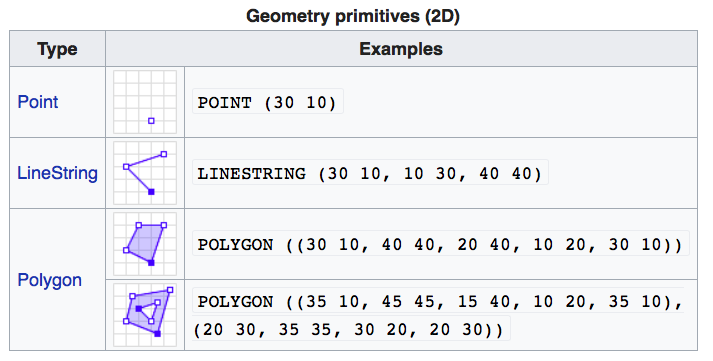
\includegraphics[width=1\linewidth]{img/wkt_primitives} \caption{Well-Known-Text Geometry primitives  (wikipedia)}\label{fig:wkt-primitives}
\end{figure}

\begin{figure}
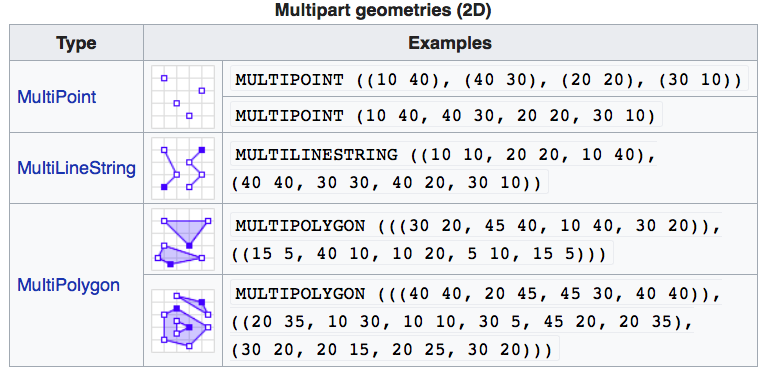
\includegraphics[width=1\linewidth]{img/wkt_multipart} \caption{Well-Known-Text Multipart geometries (wikipedia)}\label{fig:wkt-multipart}
\end{figure}

\texttt{sf} implements this standard natively in R. Data are structured
and conceptualized very differently from the \texttt{sp} approach.

In \texttt{sf} spatial objects are stored as a simple data frame with a
special column that contains the information for the geometry
coordinates. That special column is a list with the same length as the
number of rows in the data frame. Each of the individual list elements
then can be of any length needed to hold the coordinates that correspond
to an individual feature.

To create a spatial \texttt{sf} object manually the basic steps would
be:

\begin{quote}
\textbf{I. Create geometric objects (topology)}
\end{quote}

Geometric objects (simple features) can be created from a numeric
vector, matrix or a list with the coordinates. They are called
\texttt{sfg} objects for Simple Feature Geometry.b Similarly to
\texttt{sp} there are functions that help create simple feature
geometries, like \texttt{st\_point()}, \texttt{st\_linestring()},
\texttt{st\_polygon()} and more.

\begin{quote}
\textbf{II. Combine all individual single feature objects for the
special column.}
\end{quote}

The feature geometries are then combined into a Simple Feature
Collection with \texttt{st\_sfc()}. which is nothing other than a simple
feature geometry list-column. The \texttt{sfc} object also holds the
bounding box and the projection information.

\begin{quote}
\begin{enumerate}
\def\labelenumi{\Roman{enumi}.}
\setcounter{enumi}{2}
\tightlist
\item
  Add attributes.
\end{enumerate}
\end{quote}

Lastly, we add the attributes to the the simple feature collection with
the \texttt{st\_sf()} function. This function extends the well known
data frame in R with a column that holds the simple feature collection.

So if we created the same highway object from above as \texttt{sf}
object we would first generate LINESTRINGs as simple feature geometries
out of a matrix with coordinates:

\begin{Shaded}
\begin{Highlighting}[]
\NormalTok{lnstr_sfg1 <-}\StringTok{ }\KeywordTok{st_linestring}\NormalTok{(}\KeywordTok{matrix}\NormalTok{(}\KeywordTok{runif}\NormalTok{(}\DecValTok{6}\NormalTok{), }\DataTypeTok{ncol=}\DecValTok{2}\NormalTok{)) }
\NormalTok{lnstr_sfg2 <-}\StringTok{ }\KeywordTok{st_linestring}\NormalTok{(}\KeywordTok{matrix}\NormalTok{(}\KeywordTok{runif}\NormalTok{(}\DecValTok{6}\NormalTok{), }\DataTypeTok{ncol=}\DecValTok{2}\NormalTok{)) }
\KeywordTok{class}\NormalTok{(lnstr_sfg1)}
\end{Highlighting}
\end{Shaded}

\begin{verbatim}
#> [1] "XY"         "LINESTRING" "sfg"
\end{verbatim}

We would then combine this into a simple feature collection :

\begin{Shaded}
\begin{Highlighting}[]
\NormalTok{(lnstr_sfc <-}\StringTok{ }\KeywordTok{st_sfc}\NormalTok{(lnstr_sfg1, lnstr_sfg2)) }\CommentTok{# just one feature here}
\end{Highlighting}
\end{Shaded}

\begin{verbatim}
#> Geometry set for 2 features 
#> geometry type:  LINESTRING
#> dimension:      XY
#> bbox:           xmin: 0.1472823 ymin: 0.03795971 xmax: 0.6951138 ymax: 0.9930134
#> epsg (SRID):    NA
#> proj4string:    NA
\end{verbatim}

\begin{verbatim}
#> LINESTRING (0.6951138 0.3978693, 0.2638811 0.03...
\end{verbatim}

\begin{verbatim}
#> LINESTRING (0.4910172 0.1953684, 0.4145963 0.30...
\end{verbatim}

And lastly use our data frame from above to generate the \texttt{sf}
object:

\begin{Shaded}
\begin{Highlighting}[]
\NormalTok{(lnstr_sf <-}\StringTok{ }\KeywordTok{st_sf}\NormalTok{(dfr , lnstr_sfc))}
\end{Highlighting}
\end{Shaded}

\begin{verbatim}
#> Simple feature collection with 2 features and 2 fields
#> geometry type:  LINESTRING
#> dimension:      XY
#> bbox:           xmin: 0.1472823 ymin: 0.03795971 xmax: 0.6951138 ymax: 0.9930134
#> epsg (SRID):    NA
#> proj4string:    NA
#>     id cars_per_hour                      lnstr_sfc
#> 1 hwy1            78 LINESTRING (0.6951138 0.397...
#> 2 hwy2            22 LINESTRING (0.4910172 0.195...
\end{verbatim}

There are many methods available in the \texttt{sf} package, to find out
use

\begin{Shaded}
\begin{Highlighting}[]
\KeywordTok{methods}\NormalTok{(}\DataTypeTok{class=}\StringTok{"sf"}\NormalTok{)}
\end{Highlighting}
\end{Shaded}

\begin{verbatim}
#>  [1] [                     [[<-                  $<-                  
#>  [4] aggregate             anti_join             arrange              
#>  [7] as.data.frame         cbind                 coerce               
#> [10] dbDataType            dbWriteTable          distinct             
#> [13] extent                extract               filter               
#> [16] full_join             group_by              identify             
#> [19] initialize            inner_join            left_join            
#> [22] mask                  merge                 mutate               
#> [25] plot                  print                 raster               
#> [28] rasterize             rbind                 rename               
#> [31] right_join            sample_frac           sample_n             
#> [34] select                semi_join             show                 
#> [37] slice                 slotsFromS3           st_agr               
#> [40] st_agr<-              st_area               st_as_sf             
#> [43] st_bbox               st_boundary           st_buffer            
#> [46] st_cast               st_centroid           st_collection_extract
#> [49] st_convex_hull        st_coordinates        st_crop              
#> [52] st_crs                st_crs<-              st_difference        
#> [55] st_geometry           st_geometry<-         st_intersection      
#> [58] st_is                 st_line_merge         st_nearest_points    
#> [61] st_node               st_point_on_surface   st_polygonize        
#> [64] st_precision          st_segmentize         st_set_precision     
#> [67] st_simplify           st_snap               st_sym_difference    
#> [70] st_transform          st_triangulate        st_union             
#> [73] st_voronoi            st_wrap_dateline      st_write             
#> [76] st_zm                 summarise             transmute            
#> [79] ungroup              
#> see '?methods' for accessing help and source code
\end{verbatim}

Here are some of the other highlights of \texttt{sf} you might be
interested in:

\begin{itemize}
\item
  provides \textbf{fast} I/O, particularly relevant for large files
\item
  spatial fuctions that rely on GEOS and GDAL and PROJ external
  libraries are directluy linked into the package, so no need to load
  additional external packages (like in \texttt{sp})\\
\item
  \texttt{sf} objects can be plotted directly with \texttt{ggplot}
\item
  \texttt{sf} directly reads from and writes to spatial
  \textbf{databases} such as PostGIS
\item
  \texttt{sf} is compatible with the
  \href{https://www.tidyverse.org/}{\texttt{tidyvderse} approach}, (but
  see some
  \href{https://geocompr.github.io/geocompkg/articles/tidyverse-pitfalls.html}{pitfalls
  here})
\end{itemize}

Note that \texttt{sp} and \texttt{sf} are not the only way spatial
objects are conceptualized in R. Other spatial packages may use their
own class definitions for spatial data (for example \texttt{spatstat}).

There are packages specifically for the
\href{https://tools.ietf.org/html/rfc7946}{GeoJSON} and for that reason
are more lightweight, for example:

\begin{itemize}
\tightlist
\item
  \href{https://cran.r-project.org/package=geojson}{\texttt{geojson}}
  and\\
\item
  \href{https://CRAN.R-project.org/package=geoops}{\texttt{geoops}} -
  (\href{https://cran.r-project.org/web/packages/geoops/vignettes/geoops_vignette.html}{demo})
\end{itemize}

Usuallly you can find functions that convert objects to and from these
formats.

\begin{quote}
Challenge

Similarly to the example above generate a Point object in R. Use both,
the \texttt{sp} and the \texttt{sf} ``approach''.

\begin{enumerate}
\def\labelenumi{\arabic{enumi}.}
\tightlist
\item
  Create a matrix \texttt{pts} of random numbers with two columns and as
  many rows as you like. These are your points.
\item
  Create a dataframe \texttt{attrib\_df} with the same number of rows as
  your \texttt{pts} matrix and a column that holds an attribute. You can
  make up any attribute.
\item
  Use the appropriate commands and \texttt{pts} to create
\end{enumerate}

\begin{itemize}
\tightlist
\item
  a \texttt{SpatialPointsDataFrame} and
\item
  an \texttt{sf} object with a gemoetry column of class
  \texttt{sfc\_POINT}.
\end{itemize}

\begin{enumerate}
\def\labelenumi{\arabic{enumi}.}
\setcounter{enumi}{3}
\tightlist
\item
  Try to subset your spatial object using the attribute you have added
  and the way you are used to from regular data frames.
\item
  How do you determine the bounding box of your spatial object?
\end{enumerate}
\end{quote}

\section{Creating a spatial object from a lat/lon
table}\label{creating-a-spatial-object-from-a-latlon-table}

Often in your research might have a spreadsheet that contains latitude,
longitude and perhaps some attribute values. You know how to read the
spreadsheet into a data frame with \texttt{read.table} or
\texttt{read.csv}. We can then very easily convert the table into a
spatial object in R.

\subsection{\texorpdfstring{With \texttt{sf}}{With sf}}\label{with-sf}

An \texttt{sf} object can be created from a data frame in the following
way. We take advantage of the \texttt{st\_as\_sf()} function which
converts any foreign object into an \texttt{sf} object. Similarly to
above, it requires an argument \texttt{coords}, which in the case of
point data needs to be a vector that specifies the data frame's columns
for the longitude and latitude (x,y) coordinates.

\begin{verbatim}
my_sf_object <- st_as_sf(myDataframe, coords)
\end{verbatim}

\texttt{st\_as\_sf()} creates a new object and leaves the original data
frame untouched.

We use \texttt{read.csv()} to read \texttt{philly\_homicides.csv} into a
dataframe in R and name it \texttt{philly\_homicides\_df}.

\begin{Shaded}
\begin{Highlighting}[]
\NormalTok{philly_homicides_df <-}\StringTok{ }\KeywordTok{read.csv}\NormalTok{(}\StringTok{"data/philly_homicides.csv"}\NormalTok{)}
\KeywordTok{str}\NormalTok{(philly_homicides_df )}
\end{Highlighting}
\end{Shaded}

\begin{verbatim}
#> 'data.frame':    3883 obs. of  10 variables:
#>  $ DC_DIST          : int  22 1 1 1 1 1 1 1 1 1 ...
#>  $ SECTOR           : Factor w/ 30 levels "1","2","3","4",..: 1 6 6 6 9 10 6 14 14 5 ...
#>  $ DISPATCH_DATE    : Factor w/ 2228 levels "2006-01-01","2006-01-02",..: 2139 10 62 90 125 132 133 139 199 211 ...
#>  $ DISPATCH_TIME    : Factor w/ 1263 levels "00:00:00","00:01:00",..: 799 1 804 561 633 981 1224 86 1063 1013 ...
#>  $ LOCATION_BLOCK   : Factor w/ 3305 levels " 100 E CHAMPLOST AVE",..: 595 745 3135 806 828 588 579 853 883 625 ...
#>  $ UCR_GENERAL      : int  100 100 100 100 100 100 100 100 100 100 ...
#>  $ OBJ_ID           : int  1 1 1 1 1 1 1 1 1 1 ...
#>  $ TEXT_GENERAL_CODE: Factor w/ 4 levels "Homicide - Criminal",..: 1 1 1 1 1 2 1 1 1 1 ...
#>  $ POINT_X          : num  -75.2 -75.2 -75.2 -75.2 -75.2 ...
#>  $ POINT_Y          : num  40 39.9 39.9 39.9 39.9 ...
\end{verbatim}

We convert the \texttt{philly\_homicides\_df} data frame into an
\texttt{sf} object with \texttt{st\_as\_sf()}

\begin{Shaded}
\begin{Highlighting}[]
\NormalTok{philly_homicides_sf <-}\StringTok{ }\KeywordTok{st_as_sf}\NormalTok{(philly_homicides_df, }\DataTypeTok{coords =} \KeywordTok{c}\NormalTok{(}\StringTok{"POINT_X"}\NormalTok{, }\StringTok{"POINT_Y"}\NormalTok{))}
\KeywordTok{str}\NormalTok{(philly_homicides_sf)}
\end{Highlighting}
\end{Shaded}

\begin{verbatim}
#> Classes 'sf' and 'data.frame':   3883 obs. of  9 variables:
#>  $ DC_DIST          : int  22 1 1 1 1 1 1 1 1 1 ...
#>  $ SECTOR           : Factor w/ 30 levels "1","2","3","4",..: 1 6 6 6 9 10 6 14 14 5 ...
#>  $ DISPATCH_DATE    : Factor w/ 2228 levels "2006-01-01","2006-01-02",..: 2139 10 62 90 125 132 133 139 199 211 ...
#>  $ DISPATCH_TIME    : Factor w/ 1263 levels "00:00:00","00:01:00",..: 799 1 804 561 633 981 1224 86 1063 1013 ...
#>  $ LOCATION_BLOCK   : Factor w/ 3305 levels " 100 E CHAMPLOST AVE",..: 595 745 3135 806 828 588 579 853 883 625 ...
#>  $ UCR_GENERAL      : int  100 100 100 100 100 100 100 100 100 100 ...
#>  $ OBJ_ID           : int  1 1 1 1 1 1 1 1 1 1 ...
#>  $ TEXT_GENERAL_CODE: Factor w/ 4 levels "Homicide - Criminal",..: 1 1 1 1 1 2 1 1 1 1 ...
#>  $ geometry         :sfc_POINT of length 3883; first list element:  'XY' num  -75.2 40
#>  - attr(*, "sf_column")= chr "geometry"
#>  - attr(*, "agr")= Factor w/ 3 levels "constant","aggregate",..: NA NA NA NA NA NA NA NA
#>   ..- attr(*, "names")= chr  "DC_DIST" "SECTOR" "DISPATCH_DATE" "DISPATCH_TIME" ...
\end{verbatim}

Note the additional \textbf{geometry} list-column which now holds the
simple feature collection with the coordinates of all the points.

To make it a complete geographical object we assign the WGS84
projection, which has the EPSG code 4326:

\begin{Shaded}
\begin{Highlighting}[]
\KeywordTok{st_crs}\NormalTok{(philly_homicides_sf)}
\end{Highlighting}
\end{Shaded}

\begin{verbatim}
#> Coordinate Reference System: NA
\end{verbatim}

\begin{Shaded}
\begin{Highlighting}[]
\KeywordTok{st_crs}\NormalTok{(philly_homicides_sf) <-}\StringTok{ }\DecValTok{4326} \CommentTok{# we can use EPSG as numeric here}
\KeywordTok{st_crs}\NormalTok{(philly_homicides_sf)}
\end{Highlighting}
\end{Shaded}

\begin{verbatim}
#> Coordinate Reference System:
#>   EPSG: 4326 
#>   proj4string: "+proj=longlat +datum=WGS84 +no_defs"
\end{verbatim}

We will save this object as a shapefile on our hard drive for later use.
(Note that by default \texttt{st\_write} checks if the file already
exists, and if so it will not overwrite it. If you need to force it to
overwrite use the option \texttt{delete\_layer\ =\ TRUE}.)

\begin{Shaded}
\begin{Highlighting}[]
\KeywordTok{st_write}\NormalTok{(philly_homicides_sf, }\StringTok{"data/PhillyHomicides"}\NormalTok{, }\DataTypeTok{driver =} \StringTok{"ESRI Shapefile"}\NormalTok{)}
\CommentTok{# to force the save: }
\KeywordTok{st_write}\NormalTok{(philly_homicides_sf, }\StringTok{"data/PhillyHomicides"}\NormalTok{, }\DataTypeTok{driver =} \StringTok{"ESRI Shapefile"}\NormalTok{, }\DataTypeTok{delete_layer =} \OtherTok{TRUE}\NormalTok{)}
\end{Highlighting}
\end{Shaded}

\subsection{\texorpdfstring{With \texttt{sp}}{With sp}}\label{with-sp}

A \texttt{SpatialPointsDataFrame} object can be created directly from a
table by specifying which columns contain the coordinates. This can be
done in one step by using the \texttt{coordinates()} function. As
mentioned above this function can be used not only to retrieve spatial
coordinates but also to set them, which is done in R fashion with:

\begin{verbatim}
coordinates(myDataframe) <- value
\end{verbatim}

\texttt{value} can have different forms -- in this context needs to be a
character vector which specifies the data frame's columns for the
longitude and latitude (x,y) coordinates.

If we use this on a data frame it automatically converts the data frame
object into a \texttt{SpatialPointsDataFrame} object.

Below, we convert the \texttt{philly\_homicides\_df} data frame into a
spatial object with using the \texttt{coordinates} function and check
with \texttt{class(philly\_homicides\_df)}again to examine which object
class the table belongs to now. Note that the \texttt{coordinates()}
function if used in this way \textbf{replaces the original data frame.}

\begin{Shaded}
\begin{Highlighting}[]
\KeywordTok{coordinates}\NormalTok{(philly_homicides_df) <-}\StringTok{ }\KeywordTok{c}\NormalTok{(}\StringTok{"POINT_X"}\NormalTok{, }\StringTok{"POINT_Y"}\NormalTok{)}
\KeywordTok{class}\NormalTok{(philly_homicides_df) }\CommentTok{# !! }
\end{Highlighting}
\end{Shaded}

\begin{verbatim}
#> [1] "SpatialPointsDataFrame"
#> attr(,"package")
#> [1] "sp"
\end{verbatim}

Assigning the projection:

\begin{Shaded}
\begin{Highlighting}[]
\KeywordTok{is.projected}\NormalTok{(philly_homicides_df) }\CommentTok{# see if a projection is defined  }
\end{Highlighting}
\end{Shaded}

\begin{verbatim}
#> [1] NA
\end{verbatim}

\begin{Shaded}
\begin{Highlighting}[]
\KeywordTok{proj4string}\NormalTok{(philly_homicides_df) <-}\StringTok{ }\KeywordTok{CRS}\NormalTok{(}\StringTok{"+init=epsg:4326"}\NormalTok{) }\CommentTok{# this is WGS84}
\KeywordTok{is.projected}\NormalTok{(philly_homicides_df) }\CommentTok{# voila! hm. wait a minute..}
\end{Highlighting}
\end{Shaded}

\begin{verbatim}
#> [1] FALSE
\end{verbatim}

To save the \texttt{sp} object out as a shapefile we need to load
another library, called \texttt{rgdal} (more on this below.)

\begin{Shaded}
\begin{Highlighting}[]
\CommentTok{# to save out using writeOGR from rgdal}
\KeywordTok{library}\NormalTok{(rgdal)}

\CommentTok{# note that we need to save the philly_homicides_df, which we converted to sp object!}
\KeywordTok{writeOGR}\NormalTok{(philly_homicides_df, }\StringTok{"data/PhillyHomicides"}\NormalTok{, }\StringTok{"PhillyHomcides"}\NormalTok{, }\DataTypeTok{driver =} \StringTok{"ESRI Shapefile"}\NormalTok{)}
\CommentTok{# to force save:}
\KeywordTok{writeOGR}\NormalTok{(philly_homicides_df, }\StringTok{"data/PhillyHomicides"}\NormalTok{, }\StringTok{"PhillyHomcides"}\NormalTok{, }\DataTypeTok{driver =} \StringTok{"ESRI Shapefile"}\NormalTok{, }\DataTypeTok{overwrite_layer =} \OtherTok{TRUE}\NormalTok{)}
\end{Highlighting}
\end{Shaded}

\section{Loading shape files into R}\label{loading-shape-files-into-r}

\subsection{\texorpdfstring{How to do this in
\texttt{sf}}{How to do this in sf}}\label{how-to-do-this-in-sf}

\texttt{sf} relies on the powerful \href{http://gdal.org}{GDAL library},
which is automatically linked in when loading \texttt{sf}. We can use
\texttt{st\_read()}, which simply takes the path of the directory with
the shapefile as argument.

\begin{Shaded}
\begin{Highlighting}[]
\CommentTok{# read in}
\NormalTok{philly_sf <-}\StringTok{ }\KeywordTok{st_read}\NormalTok{(}\StringTok{"data/Philly/"}\NormalTok{)}
\end{Highlighting}
\end{Shaded}

\begin{verbatim}
#> Reading layer `PhillyTotalPopHHinc' from data source `/Users/cengel/Anthro/R_Class/R_Workshops/R-spatial/data/Philly' using driver `ESRI Shapefile'
#> Simple feature collection with 384 features and 17 fields
#> geometry type:  MULTIPOLYGON
#> dimension:      XY
#> bbox:           xmin: 1739497 ymin: 457343.7 xmax: 1764030 ymax: 490544.9
#> epsg (SRID):    NA
#> proj4string:    +proj=aea +lat_1=29.5 +lat_2=45.5 +lat_0=37.5 +lon_0=-96 +x_0=0 +y_0=0 +ellps=GRS80 +units=m +no_defs
\end{verbatim}

\begin{Shaded}
\begin{Highlighting}[]
\CommentTok{# take a look at what we've got}
\KeywordTok{str}\NormalTok{(philly_sf) }\CommentTok{# note again the geometry column}
\end{Highlighting}
\end{Shaded}

\begin{verbatim}
#> Classes 'sf' and 'data.frame':   384 obs. of  18 variables:
#>  $ STATEFP10 : Factor w/ 1 level "42": 1 1 1 1 1 1 1 1 1 1 ...
#>  $ COUNTYFP10: Factor w/ 1 level "101": 1 1 1 1 1 1 1 1 1 1 ...
#>  $ TRACTCE10 : Factor w/ 384 levels "000100","000200",..: 347 350 353 329 326 345 46 82 173 15 ...
#>  $ GEOID10   : Factor w/ 384 levels "42101000100",..: 347 350 353 329 326 345 46 82 173 15 ...
#>  $ NAME10    : Factor w/ 384 levels "1","10.01","10.02",..: 281 284 287 262 259 279 299 354 86 3 ...
#>  $ NAMELSAD10: Factor w/ 384 levels "Census Tract 1",..: 281 284 287 262 259 279 299 354 86 3 ...
#>  $ MTFCC10   : Factor w/ 1 level "G5020": 1 1 1 1 1 1 1 1 1 1 ...
#>  $ FUNCSTAT10: Factor w/ 1 level "S": 1 1 1 1 1 1 1 1 1 1 ...
#>  $ ALAND10   : num  2322732 4501110 1004313 1271533 1016206 ...
#>  $ AWATER10  : num  66075 8014 1426278 8021 0 ...
#>  $ INTPTLAT10: Factor w/ 384 levels "+39.8798897",..: 369 380 68 333 325 368 16 93 188 63 ...
#>  $ INTPTLON10: Factor w/ 384 levels "-074.9667387",..: 1 5 137 14 27 4 272 367 119 147 ...
#>  $ GISJOIN   : Factor w/ 384 levels "G4201010000100",..: 347 350 353 329 326 345 46 82 173 15 ...
#>  $ Shape_area: num  2388806 4509124 2430591 1279556 1016207 ...
#>  $ Shape_len : num  6851 10567 9257 4928 5920 ...
#>  $ medHHinc  : num  54569 NA 130139 56667 69981 ...
#>  $ totalPop  : num  3695 703 1643 4390 3807 ...
#>  $ geometry  :sfc_MULTIPOLYGON of length 384; first list element: List of 1
#>   ..$ :List of 1
#>   .. ..$ : num [1:55, 1:2] 1763647 1763473 1763366 1763378 1763321 ...
#>   ..- attr(*, "class")= chr  "XY" "MULTIPOLYGON" "sfg"
#>  - attr(*, "sf_column")= chr "geometry"
#>  - attr(*, "agr")= Factor w/ 3 levels "constant","aggregate",..: NA NA NA NA NA NA NA NA NA NA ...
#>   ..- attr(*, "names")= chr  "STATEFP10" "COUNTYFP10" "TRACTCE10" "GEOID10" ...
\end{verbatim}

Two more words about the geometry column: You can name this column any
way you wish. Secondly, you can remove this column and revert to a
regular, non-spatial data frame at any dime wiht
\texttt{st\_drop\_geometry()}.

The default \texttt{plot} of an \texttt{sf} object is a multi-plot of
the first attributes, with a warning if not all can be plotted:

\begin{Shaded}
\begin{Highlighting}[]
\KeywordTok{plot}\NormalTok{(philly_sf)}
\end{Highlighting}
\end{Shaded}

\begin{verbatim}
#> Warning: plotting the first 10 out of 17 attributes; use max.plot = 17 to
#> plot all
\end{verbatim}

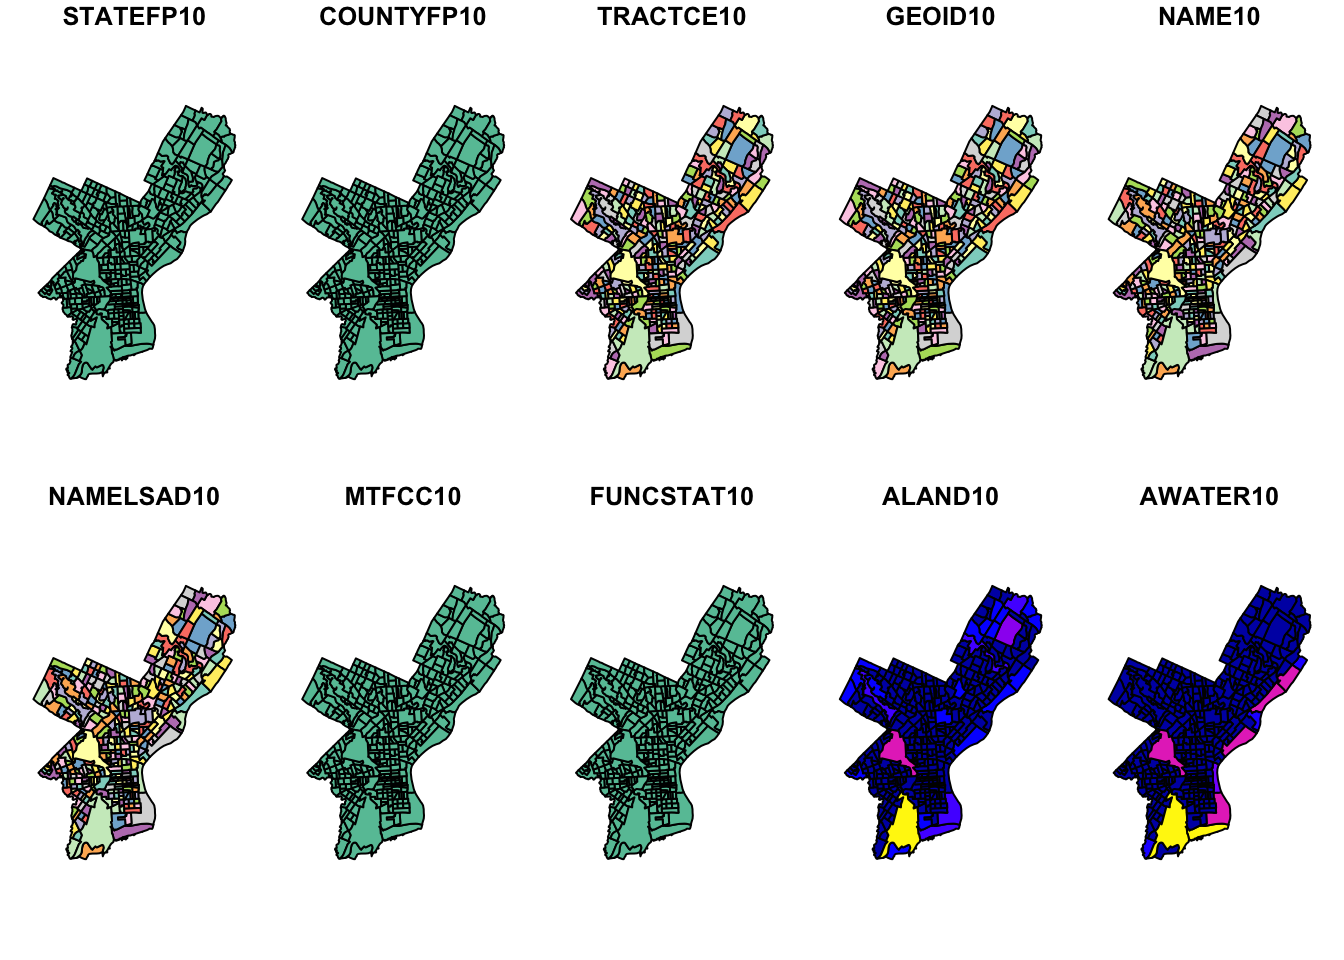
\includegraphics{R-spatial_files/figure-latex/plot-shp-sf-1.pdf}

In order to only plot the polygon boundaries we need to directly use the
geometry column. We use the \texttt{st\_geometry()} function to extract
it:

\begin{Shaded}
\begin{Highlighting}[]
\KeywordTok{plot}\NormalTok{(}\KeywordTok{st_geometry}\NormalTok{(philly_sf))}
\end{Highlighting}
\end{Shaded}

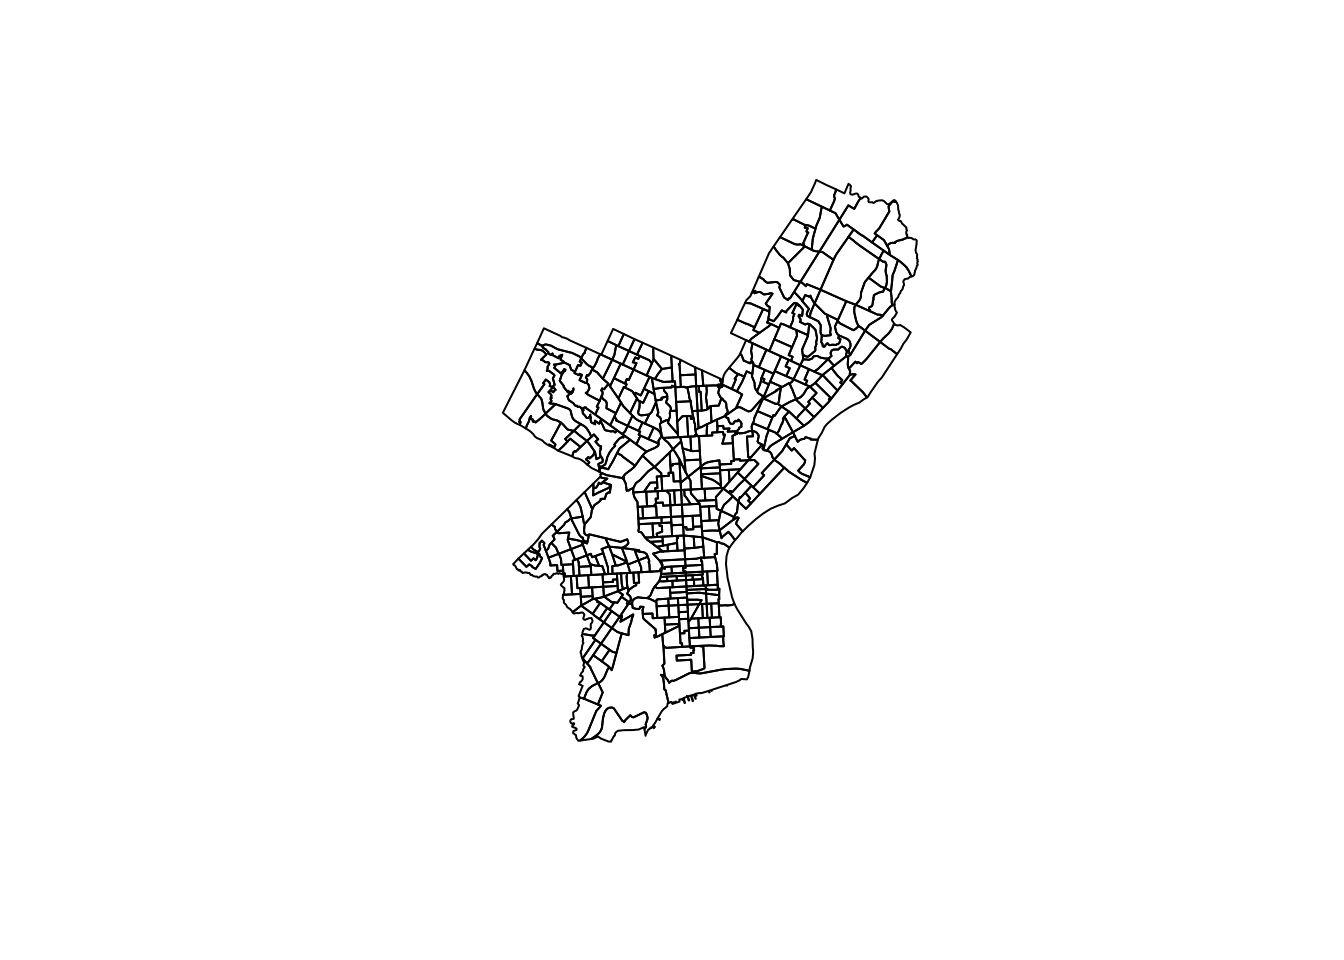
\includegraphics{R-spatial_files/figure-latex/plot-shp-sfg-1.pdf}

Let's add a subset of polygons with only the census tracts where the
median houshold income is more than \$60,000. We can extract elements
from an \texttt{sf} object based on attributes using your prefered
method of subsetting data frames.

\begin{Shaded}
\begin{Highlighting}[]
\CommentTok{# subset the familar way}
\NormalTok{philly_sf_rich <-}\StringTok{ }\NormalTok{philly_sf[philly_sf}\OperatorTok{$}\NormalTok{medHHinc }\OperatorTok{>}\StringTok{ }\DecValTok{60000}\NormalTok{, ]    }
\CommentTok{# or }
\NormalTok{philly_sf_rich <-}\StringTok{ }\KeywordTok{subset}\NormalTok{(philly_sf, medHHinc }\OperatorTok{>}\StringTok{ }\DecValTok{60000}\NormalTok{)}

\KeywordTok{plot}\NormalTok{(}\KeywordTok{st_geometry}\NormalTok{(philly_sf_rich), }\DataTypeTok{add=}\NormalTok{T, }\DataTypeTok{col=}\StringTok{"red"}\NormalTok{)}
\end{Highlighting}
\end{Shaded}

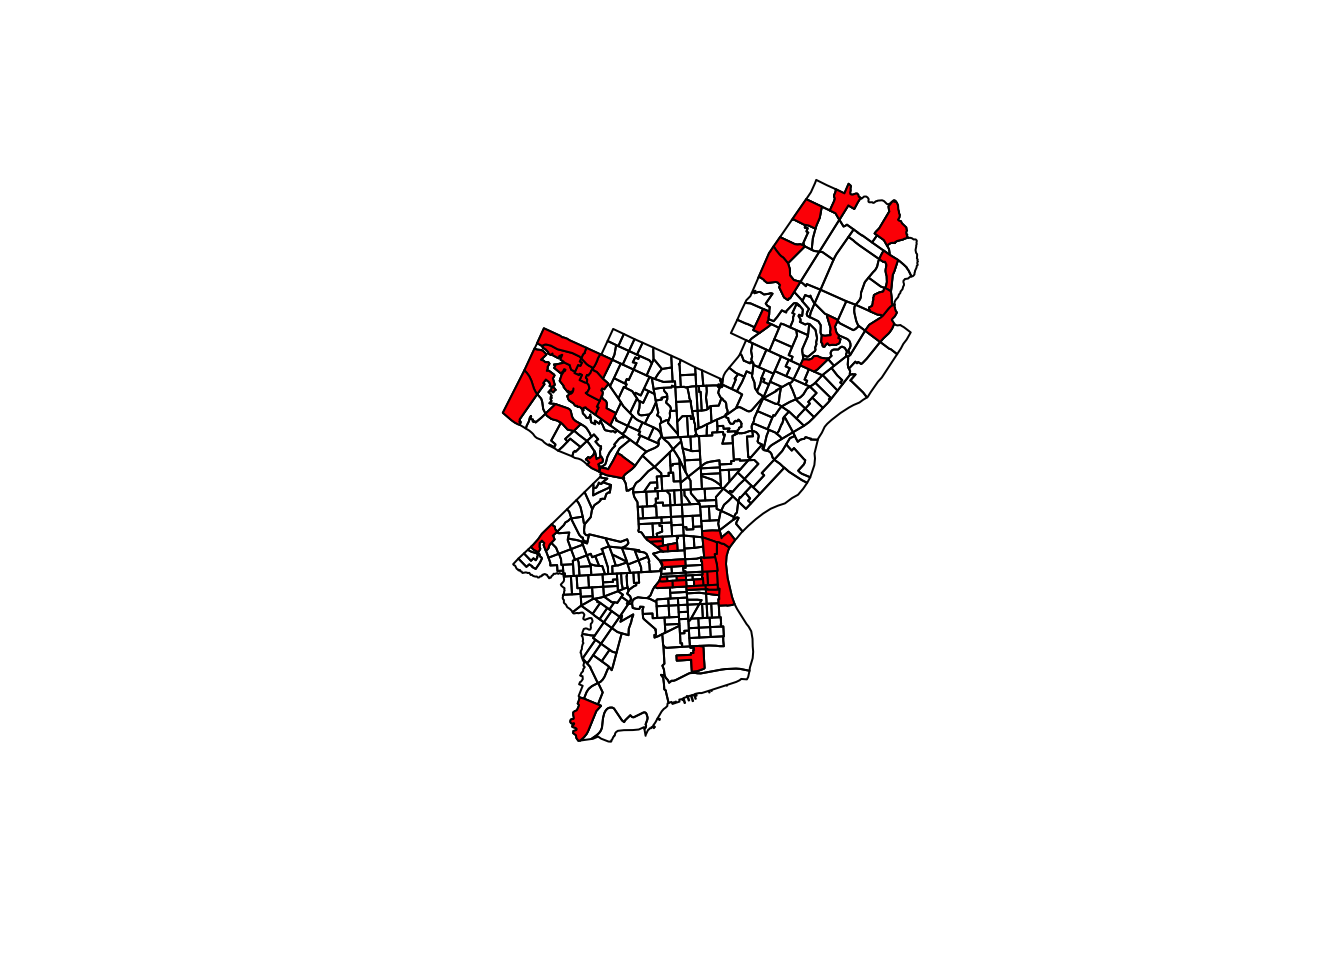
\includegraphics{R-spatial_files/figure-latex/make-subset-plot-shp-sfg-1.pdf}

Piping works as well!

\begin{Shaded}
\begin{Highlighting}[]
\KeywordTok{library}\NormalTok{(dplyr)}
\NormalTok{philly_sf }\OperatorTok\StringTok{ }
\StringTok{  }\KeywordTok{filter}\NormalTok{(medHHinc }\OperatorTok{>}\StringTok{ }\DecValTok{60000}\NormalTok{) }\OperatorTok\StringTok{ }
\StringTok{  }\KeywordTok{st_geometry}\NormalTok{() }\OperatorTok\StringTok{ }
\StringTok{  }\KeywordTok{plot}\NormalTok{(}\DataTypeTok{col=}\StringTok{"red"}\NormalTok{, }\DataTypeTok{add=}\NormalTok{T)}
\end{Highlighting}
\end{Shaded}

\subsection{\texorpdfstring{How to work with \texttt{rgdal} and
\texttt{sp}}{How to work with rgdal and sp}}\label{how-to-work-with-rgdal-and-sp}

In order to read spatial data into R and turn them into
\texttt{Spatial*} family objects we require the \texttt{rgdal} package,
which provides bindings to GDAL\footnote{GDAL supports over 200
  \href{http://www.gdal.org/formats_list.html}{raster formats} and
  \href{http://www.gdal.org/ogr_formats.html}{vector formats}. Use
  \texttt{ogrDrivers()} and \texttt{gdalDrivers()} (without arguments)
  to find out which formats your \texttt{rgdal} install can handle.}.

We can read in and write out spatial data using:

\begin{verbatim}
readOGR() and writeOGR() (for vector)  
readGDAL() and writeGDAL() (for raster/grids)
\end{verbatim}

The parameters provided for each function vary depending on the exact
spatial file type you are reading. We will take an ESRI shapefile as an
example. A shapefile - as you know -
\href{https://en.wikipedia.org/wiki/Shapefile}{consists of various files
of the same name, but with different extensions}. They should all be in
one directory and that is what R expects.

When reading in a shapefile, \texttt{readOGR()} requires the following
two arguments:

\begin{verbatim}
datasource name (dsn)  # the path to the folder that contains the files
                       # this is a path to the folder, not a filename!
layer name (layer)     # the shapefile name WITHOUT extension
                       # this is not a path but just the name of the file!
\end{verbatim}

Setting these arguments correctly can be cause of much headache for
beginners, so let me spell it out:

\begin{itemize}
\item
  Firstly, you obviously need to know the name of shapefile.
\item
  Secondly, you need to know the name and location of the folder that
  contains all the shapefile parts.
\item
  Lastly, \texttt{readOGR} only reads the file and dumps it on your
  screen. But similarly when reading csv tables you want to actually
  work with the file, so you need to assign it to an R object.
\end{itemize}

Now let's do this.

We load the \texttt{rgdal} package and read \texttt{PhillyTotalPopHHinc}
into an object called \texttt{philly} by using the \texttt{readOGR}
function\footnote{Unlike read.csv readOGR does not understand the
  \texttt{\textasciitilde{}} as valid element of a path. This (on Mac)
  will not work:
  \texttt{philly\_sp\ \textless{}-\ readOGR("\textasciitilde{}/Desktop/data/Philly/",\ "PhillyTotalPopHHinc")}}.
We can also examine the object and confirm what it is with
\texttt{class()}.

\begin{Shaded}
\begin{Highlighting}[]
\KeywordTok{library}\NormalTok{(rgdal)}
\NormalTok{philly_sp <-}\StringTok{ }\KeywordTok{readOGR}\NormalTok{(}\StringTok{"data/Philly/"}\NormalTok{, }\StringTok{"PhillyTotalPopHHinc"}\NormalTok{) }
\end{Highlighting}
\end{Shaded}

\begin{verbatim}
#> OGR data source with driver: ESRI Shapefile 
#> Source: "/Users/cengel/Anthro/R_Class/R_Workshops/R-spatial/data/Philly", layer: "PhillyTotalPopHHinc"
#> with 384 features
#> It has 17 fields
\end{verbatim}

\begin{Shaded}
\begin{Highlighting}[]
\KeywordTok{class}\NormalTok{(philly_sp)}
\end{Highlighting}
\end{Shaded}

\begin{verbatim}
#> [1] "SpatialPolygonsDataFrame"
#> attr(,"package")
#> [1] "sp"
\end{verbatim}

Very similarly to the above we can create a simple plot of the polygons
with the \texttt{plot} command, which directly understands the
\texttt{SpatialPolygonsDatafame} object and then plot a subset of
polygons with a median household income (\texttt{medHHinc}) of over
\$60,000 on top of the plot of the entire city.

\begin{Shaded}
\begin{Highlighting}[]
\KeywordTok{plot}\NormalTok{(philly_sp)}
\NormalTok{philly_sp_rich <-}\StringTok{ }\KeywordTok{subset}\NormalTok{(philly_sp, medHHinc }\OperatorTok{>}\StringTok{ }\DecValTok{60000}\NormalTok{)}
\KeywordTok{plot}\NormalTok{(philly_sp_rich, }\DataTypeTok{add=}\NormalTok{T, }\DataTypeTok{col=}\StringTok{"red"}\NormalTok{)}
\end{Highlighting}
\end{Shaded}

\section{Raster data in R}\label{raster-data-in-r}

Raster files, as you might know, have a much more compact data structure
than vectors. Because of their regular structure the coordinates do not
need to be recorded for each pixel or cell in the rectangular extent. A
raster is defined by:

\begin{itemize}
\tightlist
\item
  a CRS
\item
  coordinates of its origin
\item
  a distance or cell size in each direction
\item
  a dimension or numbers of cells in each direction
\item
  an array of cell values
\end{itemize}

Given this structure, coordinates for any cell can be computed and don't
need to be stored.

The \texttt{raster} package\footnote{Note that \texttt{sp} also allows
  to work with raster structures. The \texttt{GridTopology} class is the
  key element of raster representations. It contains: (a) the center
  coordinate pair of the south-west raster cell, (b) the two cell sizes
  in the metric of the coordinates, giving the step to successive
  centres, and (c) the numbers of cells for each dimension. There is
  also a \texttt{SpatialPixels} object which stores grid topology and
  coordinates of the actual points.} is a major extension of spatial
data classes to access large rasters and in particular to process very
large files. It includes object classes for \texttt{RasterLayer},
\texttt{RasterStacks}, and \texttt{RasterBricks}, functions for
converting among these classes, and operators for computations on the
raster data. Conversion from \texttt{sp} type objects into
\texttt{raster} type objects is possible.

If we wanted to do create a raster object from scratch we would do the
following:

\begin{Shaded}
\begin{Highlighting}[]
\CommentTok{# specify the RasterLayer with the following parameters:}
\CommentTok{# - minimum x coordinate (left border)}
\CommentTok{# - minimum y coordinate (bottom border)}
\CommentTok{# - maximum x coordinate (right border)}
\CommentTok{# - maximum y coordinate (top border)}
\CommentTok{# - resolution (cell size) in each dimension}
\NormalTok{r <-}\StringTok{ }\KeywordTok{raster}\NormalTok{(}\DataTypeTok{xmn=}\OperatorTok{-}\FloatTok{0.5}\NormalTok{, }\DataTypeTok{ymn=}\OperatorTok{-}\FloatTok{0.5}\NormalTok{, }\DataTypeTok{xmx=}\FloatTok{4.5}\NormalTok{, }\DataTypeTok{ymx=}\FloatTok{4.5}\NormalTok{, }\DataTypeTok{resolution=}\KeywordTok{c}\NormalTok{(}\DecValTok{1}\NormalTok{,}\DecValTok{1}\NormalTok{))}
\NormalTok{r}
\end{Highlighting}
\end{Shaded}

\begin{verbatim}
#> class       : RasterLayer 
#> dimensions  : 5, 5, 25  (nrow, ncol, ncell)
#> resolution  : 1, 1  (x, y)
#> extent      : -0.5, 4.5, -0.5, 4.5  (xmin, xmax, ymin, ymax)
#> coord. ref. : +proj=longlat +datum=WGS84 +ellps=WGS84 +towgs84=0,0,0
\end{verbatim}

Note that this raster object \textbf{has a CRS defined!} If the crs
argument is missing when creating the Raster object, the x coordinates
are within -360 and 360 and the y coordinates are within -90 and 90, the
WGS84 projection is used by default!

Good to know.

To add some values to the cells we could the following.

\begin{Shaded}
\begin{Highlighting}[]
\KeywordTok{class}\NormalTok{(r)}
\end{Highlighting}
\end{Shaded}

\begin{verbatim}
#> [1] "RasterLayer"
#> attr(,"package")
#> [1] "raster"
\end{verbatim}

\begin{Shaded}
\begin{Highlighting}[]
\NormalTok{r <-}\StringTok{ }\KeywordTok{setValues}\NormalTok{(r, }\KeywordTok{runif}\NormalTok{(}\DecValTok{25}\NormalTok{))}
\KeywordTok{class}\NormalTok{(r)}
\end{Highlighting}
\end{Shaded}

\begin{verbatim}
#> [1] "RasterLayer"
#> attr(,"package")
#> [1] "raster"
\end{verbatim}

\begin{Shaded}
\begin{Highlighting}[]
\KeywordTok{plot}\NormalTok{(r); }\KeywordTok{points}\NormalTok{(}\KeywordTok{coordinates}\NormalTok{(r), }\DataTypeTok{pch=}\DecValTok{3}\NormalTok{)}
\end{Highlighting}
\end{Shaded}

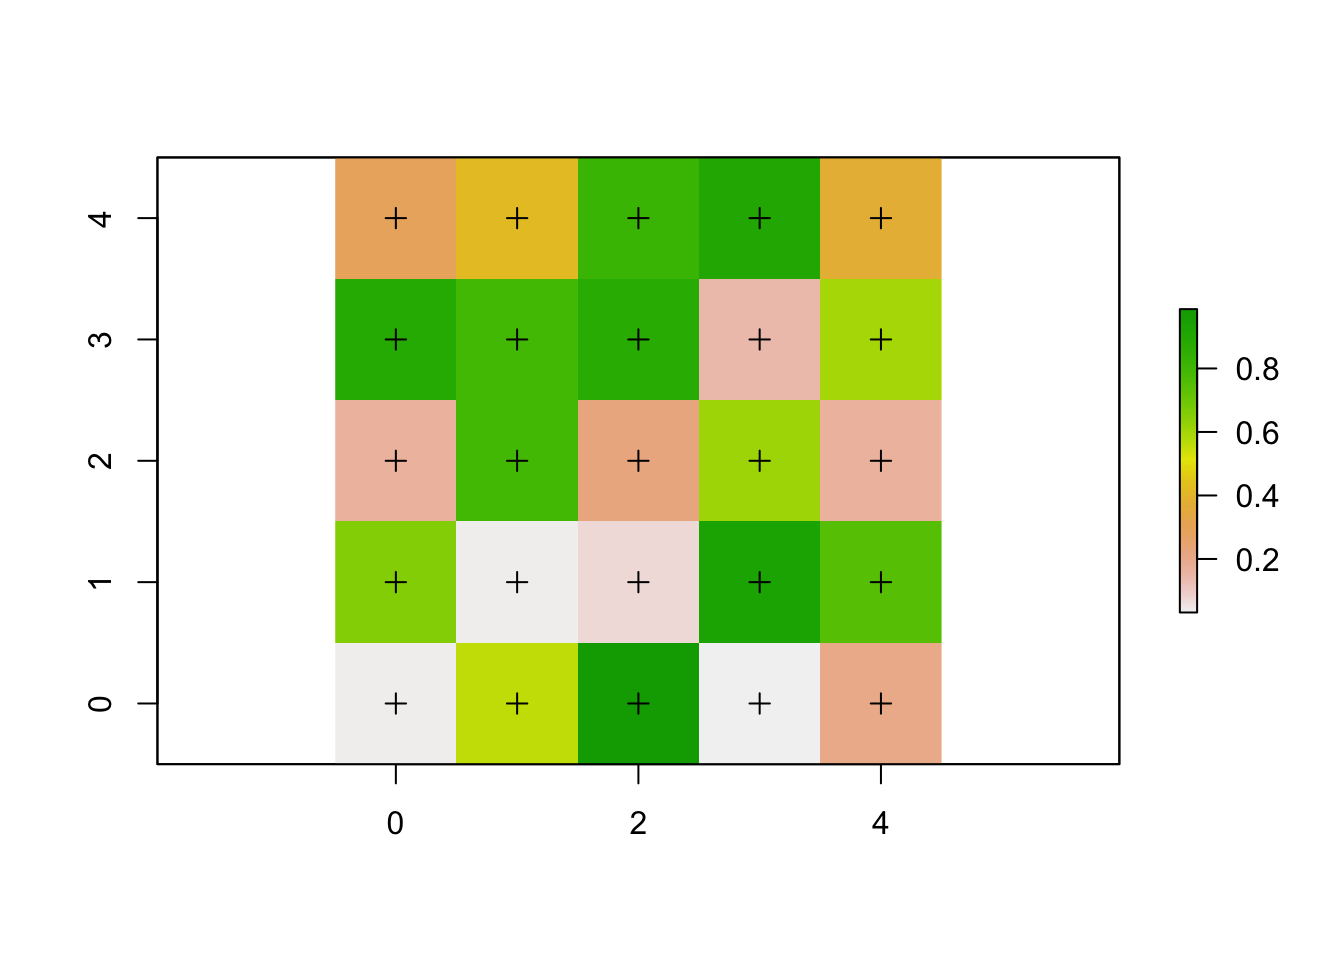
\includegraphics{R-spatial_files/figure-latex/unnamed-chunk-6-1.pdf}

(See the
\href{https://cran.r-project.org/web/packages/rasterVis/index.html}{\texttt{rasterVis}
package} for more advanced plotting of \texttt{Raster*} objects.)

RasterLayer objects can also be created from a matrix.

\begin{Shaded}
\begin{Highlighting}[]
\KeywordTok{class}\NormalTok{(volcano)}
\end{Highlighting}
\end{Shaded}

\begin{verbatim}
#> [1] "matrix"
\end{verbatim}

\begin{Shaded}
\begin{Highlighting}[]
\NormalTok{volcano.r <-}\StringTok{ }\KeywordTok{raster}\NormalTok{(volcano)}
\KeywordTok{class}\NormalTok{(volcano.r)}
\end{Highlighting}
\end{Shaded}

\begin{verbatim}
#> [1] "RasterLayer"
#> attr(,"package")
#> [1] "raster"
\end{verbatim}

And to read in a raster file we can use the \texttt{raster()} function.
This raster is generated as part of the
\href{https://www.neonscience.org/field-sites/field-sites-map/HARV}{NEON
Harvard Forest field site}.

\begin{Shaded}
\begin{Highlighting}[]
\KeywordTok{library}\NormalTok{(raster)}
\NormalTok{HARV <-}\StringTok{ }\KeywordTok{raster}\NormalTok{(}\StringTok{"data/HARV_RGB_Ortho.tif"}\NormalTok{)}
\end{Highlighting}
\end{Shaded}

Typing the name of the object will give us what's in there:

\begin{Shaded}
\begin{Highlighting}[]
\NormalTok{HARV}
\end{Highlighting}
\end{Shaded}

\begin{verbatim}
#> class       : RasterLayer 
#> band        : 1  (of  3  bands)
#> dimensions  : 2317, 3073, 7120141  (nrow, ncol, ncell)
#> resolution  : 0.25, 0.25  (x, y)
#> extent      : 731998.5, 732766.8, 4712956, 4713536  (xmin, xmax, ymin, ymax)
#> coord. ref. : +proj=utm +zone=18 +datum=WGS84 +units=m +no_defs +ellps=WGS84 +towgs84=0,0,0 
#> data source : /Users/cengel/Anthro/R_Class/R_Workshops/R-spatial/data/HARV_RGB_Ortho.tif 
#> names       : HARV_RGB_Ortho 
#> values      : 0, 255  (min, max)
\end{verbatim}

We can plot it like this:

\begin{Shaded}
\begin{Highlighting}[]
\KeywordTok{plot}\NormalTok{(HARV)}
\end{Highlighting}
\end{Shaded}

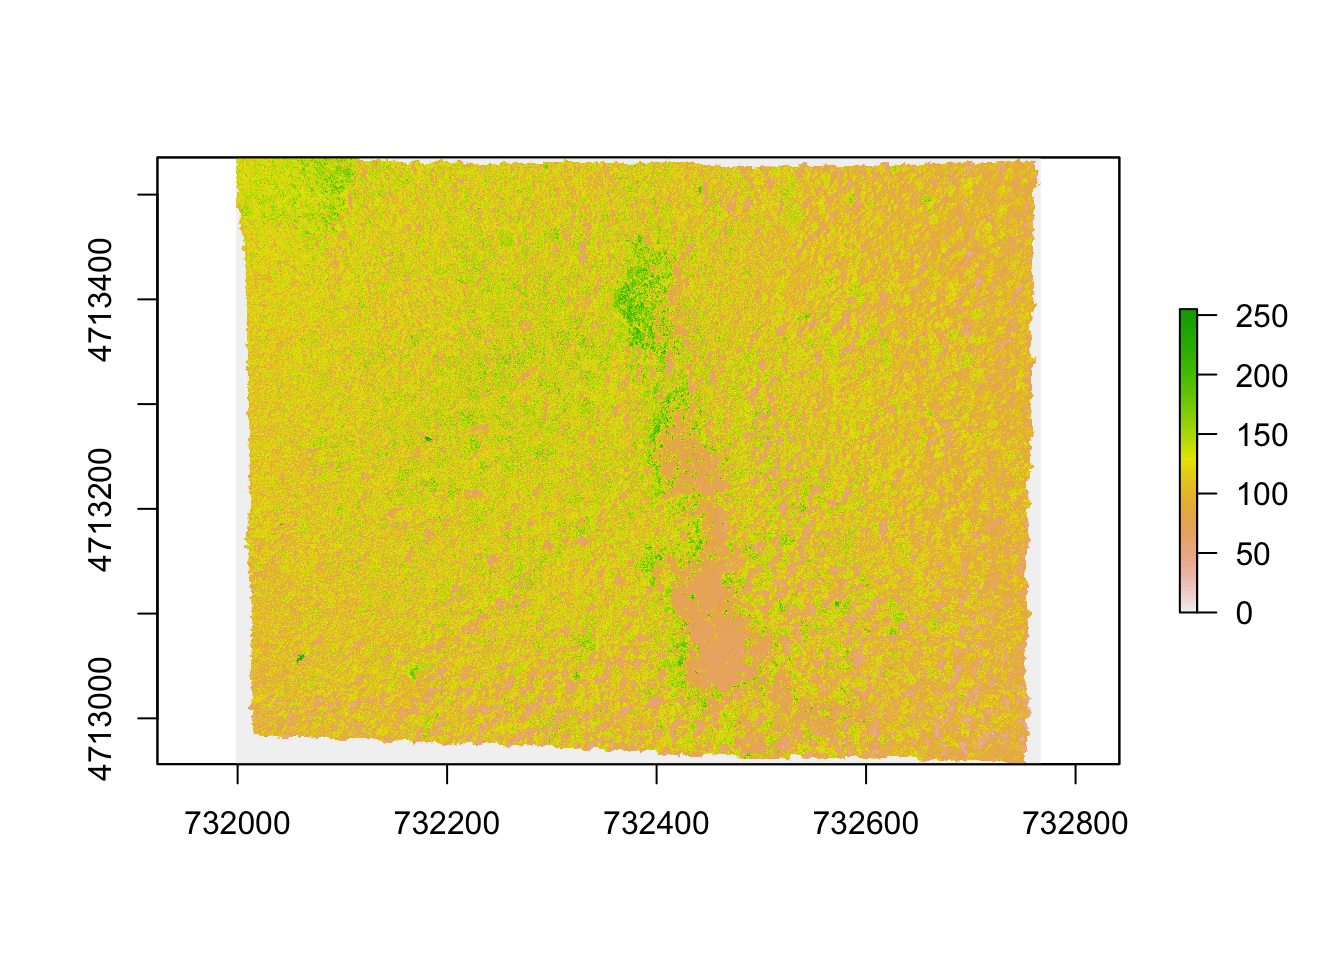
\includegraphics{R-spatial_files/figure-latex/plot-raster-1.pdf}

We can find out about the Coordinate Reference System with this:

\begin{Shaded}
\begin{Highlighting}[]
\KeywordTok{crs}\NormalTok{(HARV)}
\end{Highlighting}
\end{Shaded}

\begin{verbatim}
#> CRS arguments:
#>  +proj=utm +zone=18 +datum=WGS84 +units=m +no_defs +ellps=WGS84
#> +towgs84=0,0,0
\end{verbatim}

See what you can do with such an object:

\begin{Shaded}
\begin{Highlighting}[]
\KeywordTok{methods}\NormalTok{(}\DataTypeTok{class=}\KeywordTok{class}\NormalTok{(HARV))}
\end{Highlighting}
\end{Shaded}

\begin{verbatim}
#>   [1] !                !=               [                [[              
#>   [5] [<-              %in%             ==               $               
#>   [9] $<-              addLayer         adjacent         aggregate       
#>  [13] all.equal        area             Arith            as.array        
#>  [17] as.character     as.data.frame    as.factor        as.integer      
#>  [21] as.list          as.logical       as.matrix        as.raster       
#>  [25] as.vector        asFactor         atan2            bandnr          
#>  [29] barplot          bbox             boundaries       boxplot         
#>  [33] brick            buffer           calc             cellFromRowCol  
#>  [37] cellFromXY       cellStats        clamp            click           
#>  [41] clump            coerce           colFromCell      colFromX        
#>  [45] colSums          Compare          contour          coordinates     
#>  [49] corLocal         cover            crop             crosstab        
#>  [53] crs<-            cut              cv               density         
#>  [57] dim              dim<-            direction        disaggregate    
#>  [61] distance         extend           extent           extract         
#>  [65] flip             focal            freq             getValues       
#>  [69] getValuesBlock   getValuesFocal   gridDistance     head            
#>  [73] hist             image            interpolate      intersect       
#>  [77] is.factor        is.finite        is.infinite      is.na           
#>  [81] is.nan           isLonLat         KML              labels          
#>  [85] layerize         length           levels           levels<-        
#>  [89] lines            localFun         log              Logic           
#>  [93] mask             match            Math             Math2           
#>  [97] maxValue         mean             merge            minValue        
#> [101] modal            mosaic           names            names<-         
#> [105] ncell            ncol             ncol<-           nlayers         
#> [109] nrow             nrow<-           origin           origin<-        
#> [113] overlay          persp            plot             predict         
#> [117] print            proj4string      proj4string<-    quantile        
#> [121] raster           rasterize        readAll          readStart       
#> [125] readStop         reclassify       res              resample        
#> [129] RGB              rotate           rowColFromCell   rowFromCell     
#> [133] rowFromY         rowSums          sampleRandom     sampleRegular   
#> [137] sampleStratified scale            select           setMinMax       
#> [141] setValues        shift            show             spplot          
#> [145] stack            stackSelect      subs             subset          
#> [149] Summary          summary          t                tail            
#> [153] text             trim             unique           update          
#> [157] values           values<-         Which            which.max       
#> [161] which.min        writeRaster      writeStart       writeStop       
#> [165] writeValues      xFromCell        xFromCol         xmax            
#> [169] xmin             xres             xyFromCell       yFromCell       
#> [173] yFromRow         ymax             ymin             yres            
#> [177] zonal            zoom            
#> see '?methods' for accessing help and source code
\end{verbatim}

We can explore the distribution of values contained within our raster
using the hist() function which produces a histogram. Histograms are
often useful in identifying outliers and bad data values in our raster
data.

\begin{Shaded}
\begin{Highlighting}[]
\KeywordTok{hist}\NormalTok{(HARV)}
\end{Highlighting}
\end{Shaded}

\begin{verbatim}
#> Warning in .hist1(x, maxpixels = maxpixels, main = main, plot = plot, ...):
#> 1% of the raster cells were used. 100000 values used.
\end{verbatim}

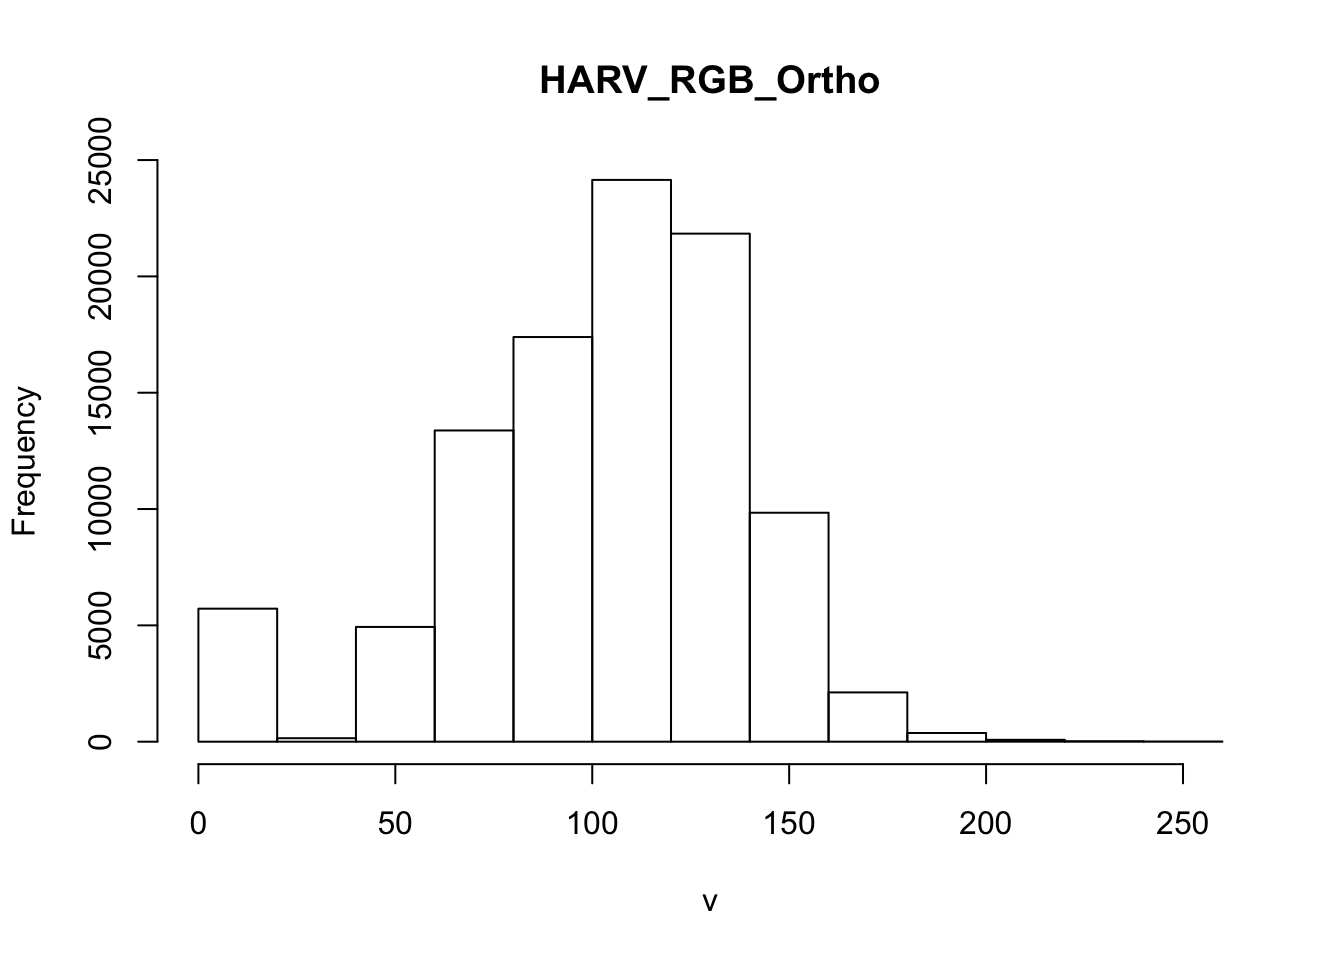
\includegraphics{R-spatial_files/figure-latex/n-hist-1.pdf}

Notice that a warning message is produced when R creates the histogram.

This warning is caused by the default maximum pixels value of 100,000
associated with the hist function. This maximum value is to ensure
processing efficiency as our data become larger! We can force the
\texttt{hist} function to use all cell values.

\begin{Shaded}
\begin{Highlighting}[]
\KeywordTok{ncell}\NormalTok{(HARV)}
\end{Highlighting}
\end{Shaded}

\begin{verbatim}
#> [1] 7120141
\end{verbatim}

\begin{Shaded}
\begin{Highlighting}[]
\KeywordTok{hist}\NormalTok{(HARV, }\DataTypeTok{maxpixels =} \KeywordTok{ncell}\NormalTok{(HARV))}
\end{Highlighting}
\end{Shaded}

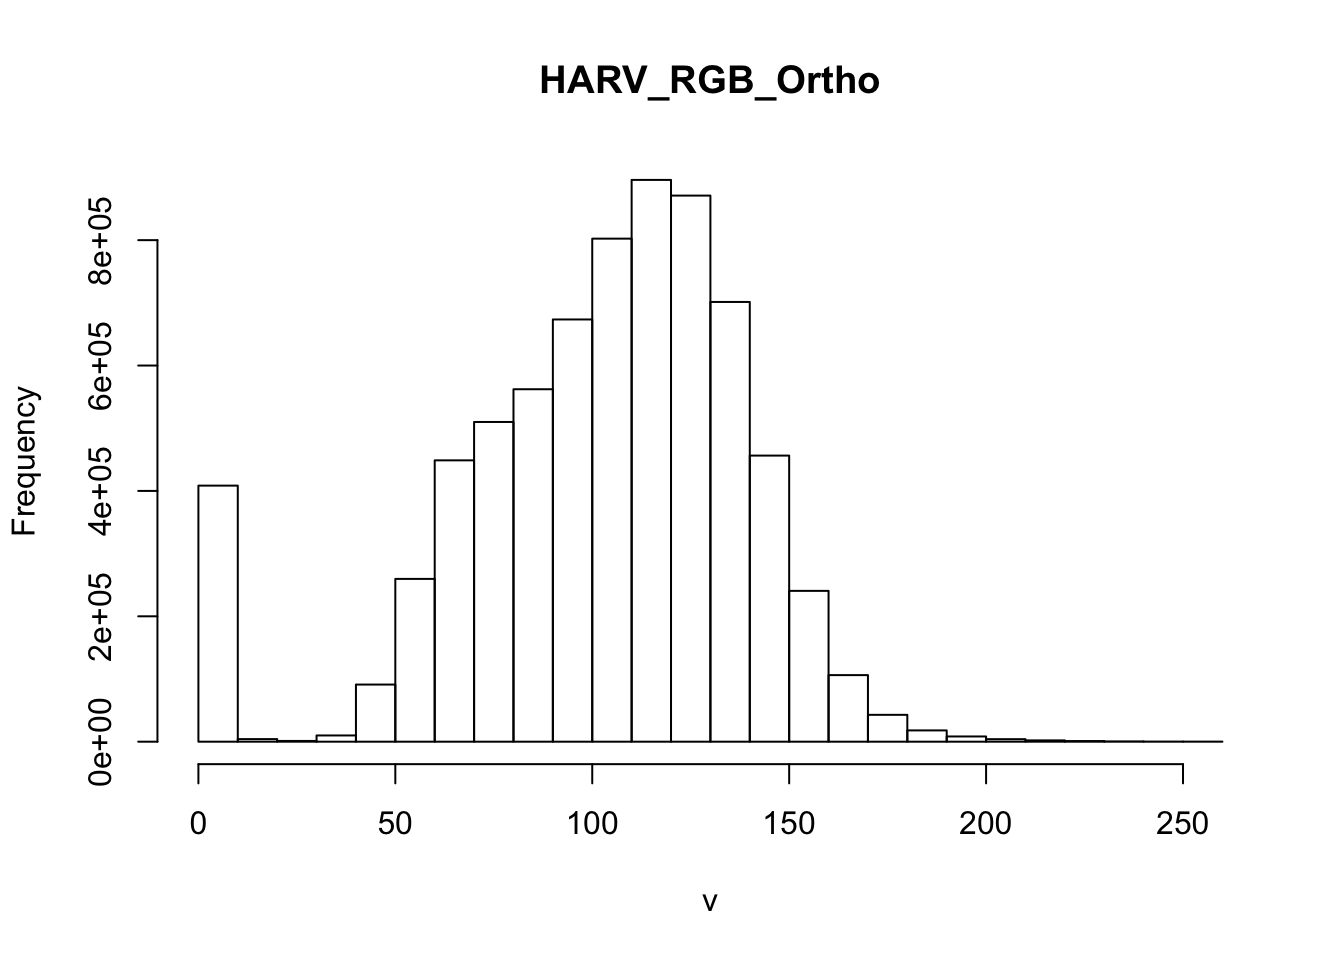
\includegraphics{R-spatial_files/figure-latex/n-hist-allvals-1.pdf}

At times it may be useful to explore raster metadata before loading them
into R. This can be done with:

\begin{verbatim}
GDALinfo("path-to-raster-here") 
\end{verbatim}

A raster dataset can contain one or more bands. We can view the number
of bands in a raster using the \texttt{nlayers()} function.

\begin{Shaded}
\begin{Highlighting}[]
\KeywordTok{nlayers}\NormalTok{(HARV)}
\end{Highlighting}
\end{Shaded}

\begin{verbatim}
#> [1] 1
\end{verbatim}

We can use the \texttt{raster()} function to import one single band from
a \emph{single} \textbf{OR} from a \emph{multi-band} raster. For
multi-band raster, we can specify which band we want to read in.

\begin{Shaded}
\begin{Highlighting}[]
\NormalTok{HARV_Band2 <-}\StringTok{ }\KeywordTok{raster}\NormalTok{(}\StringTok{"data/HARV_RGB_Ortho.tif"}\NormalTok{, }\DataTypeTok{band =} \DecValTok{2}\NormalTok{)}
\KeywordTok{plot}\NormalTok{(HARV_Band2)}
\end{Highlighting}
\end{Shaded}

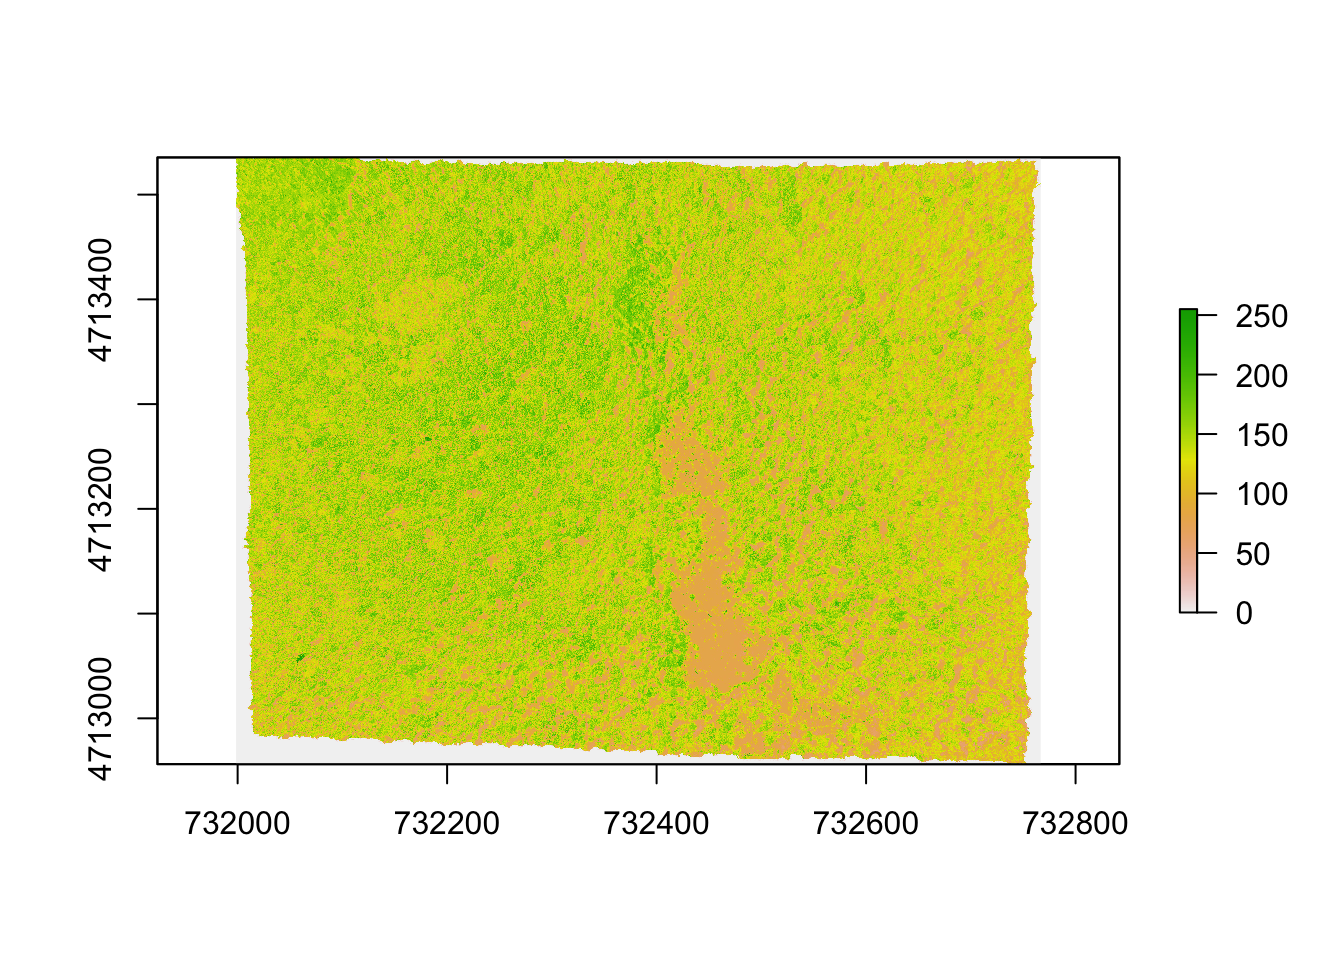
\includegraphics{R-spatial_files/figure-latex/one-multiband-1.pdf}

To bring in all bands of a multi-band raster, we use the
\texttt{stack()} function.

\begin{Shaded}
\begin{Highlighting}[]
\NormalTok{HARV_stack <-}\StringTok{ }\KeywordTok{stack}\NormalTok{(}\StringTok{"data/HARV_RGB_Ortho.tif"}\NormalTok{)}

\CommentTok{# how many layers?}
\KeywordTok{nlayers}\NormalTok{(HARV_stack)}
\end{Highlighting}
\end{Shaded}

\begin{verbatim}
#> [1] 3
\end{verbatim}

\begin{Shaded}
\begin{Highlighting}[]
\CommentTok{# view attributes of stack object}
\NormalTok{HARV_stack}
\end{Highlighting}
\end{Shaded}

\begin{verbatim}
#> class       : RasterStack 
#> dimensions  : 2317, 3073, 7120141, 3  (nrow, ncol, ncell, nlayers)
#> resolution  : 0.25, 0.25  (x, y)
#> extent      : 731998.5, 732766.8, 4712956, 4713536  (xmin, xmax, ymin, ymax)
#> coord. ref. : +proj=utm +zone=18 +datum=WGS84 +units=m +no_defs +ellps=WGS84 +towgs84=0,0,0 
#> names       : HARV_RGB_Ortho.1, HARV_RGB_Ortho.2, HARV_RGB_Ortho.3 
#> min values  :                0,                0,                0 
#> max values  :              255,              255,              255
\end{verbatim}

What happens when we plot?

\begin{Shaded}
\begin{Highlighting}[]
\KeywordTok{plot}\NormalTok{(HARV_stack)}
\end{Highlighting}
\end{Shaded}

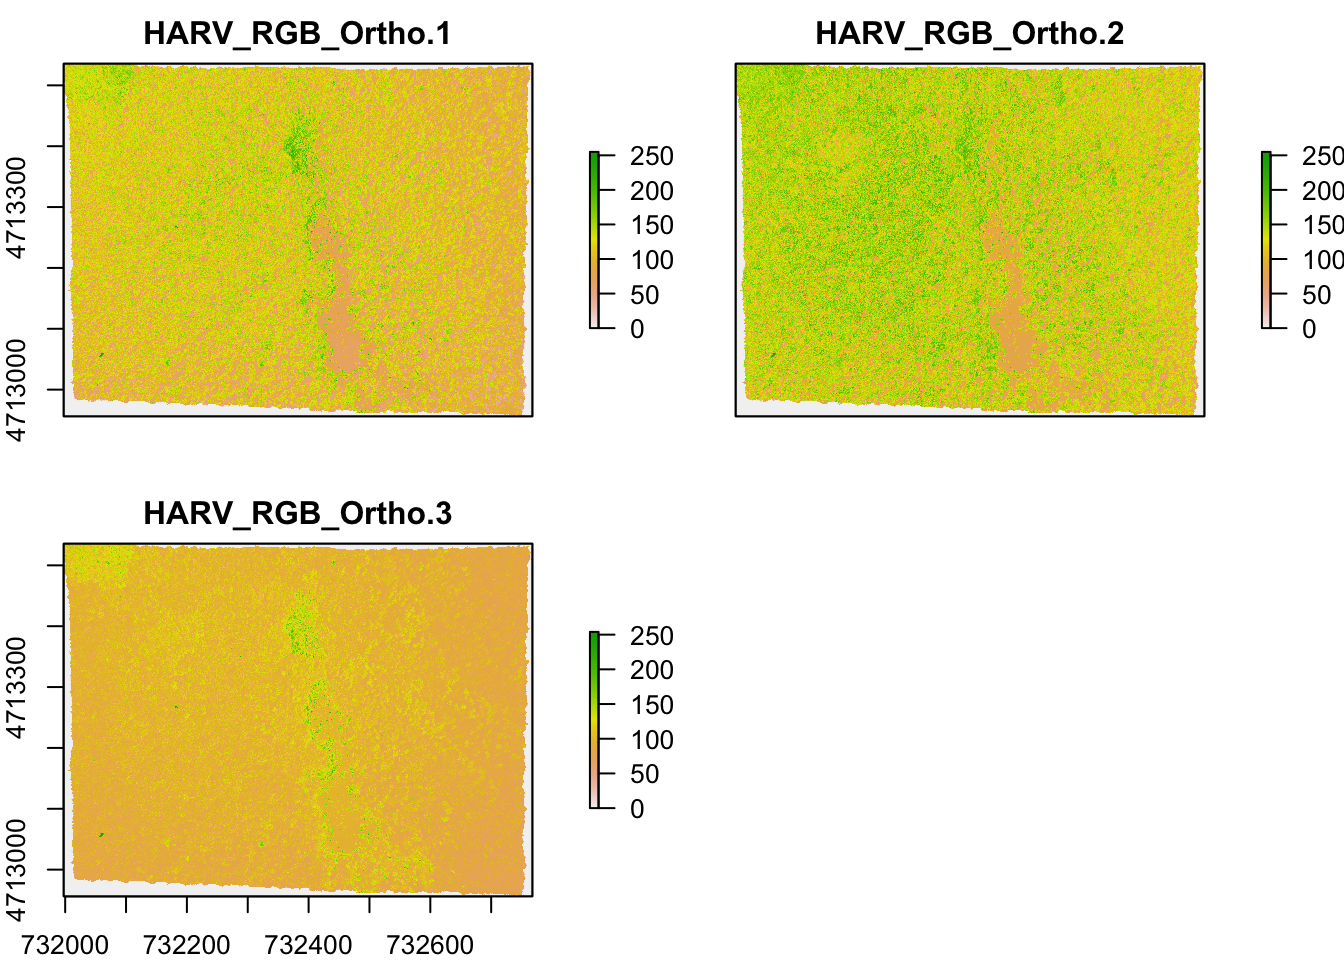
\includegraphics{R-spatial_files/figure-latex/stack-plot-1.pdf}

If we know that it is an RGB multiband raster we can plot them all in
one

\begin{Shaded}
\begin{Highlighting}[]
\KeywordTok{plotRGB}\NormalTok{(HARV_stack)}
\end{Highlighting}
\end{Shaded}

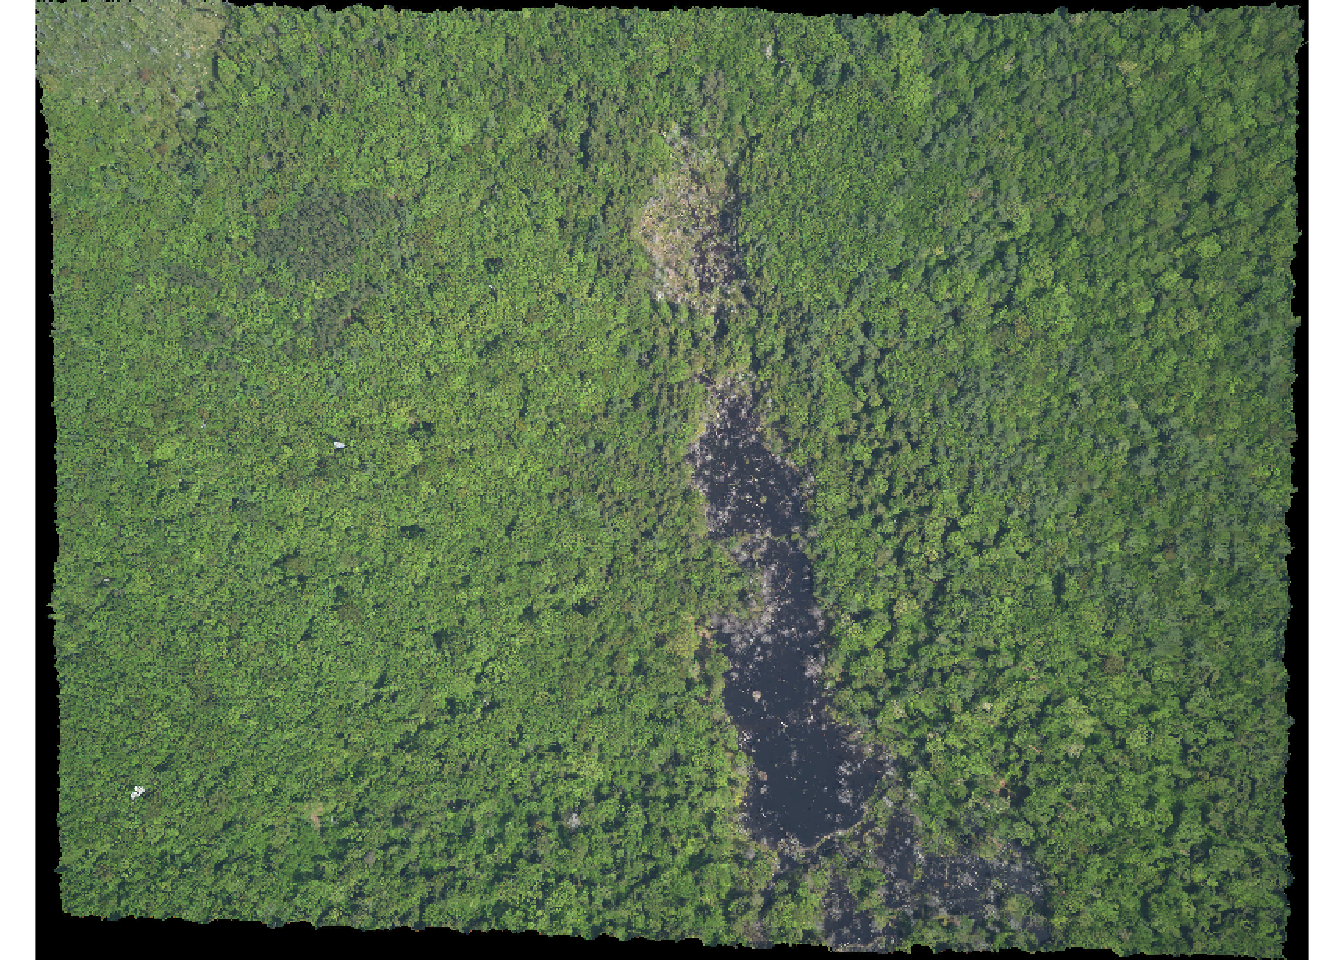
\includegraphics{R-spatial_files/figure-latex/stack-rgb-plot-1.pdf}

\subsection{RasterStack vs
RasterBrick}\label{rasterstack-vs-rasterbrick}

The R \texttt{RasterStack} and \texttt{RasterBrick} object types can
both store multiple bands. However, how they store each band is
different. The bands in a \texttt{RasterStack} are stored as links to
raster data that is located somewhere on our computer. A
\texttt{RasterBrick} contains all of the objects stored within the
actual R object. Since in the \texttt{RasterBrick}, all of the bands are
stored within the actual object its object size is much larger than the
\texttt{RasterStack} object.

In most cases, we can work with a \texttt{RasterBrick} in the same way
we might work with a \texttt{RasterStack}. However, a
\texttt{RasterBrick} is often more efficient and faster to process -
which is important when working with larger files.

We can turn a \texttt{RasterStack} into a \texttt{RasterBrick} in R by
using \texttt{brick(StackName)}. Use the \texttt{object.size()} function
to compare stack and brick R objects.

\begin{Shaded}
\begin{Highlighting}[]
\KeywordTok{object.size}\NormalTok{(HARV_stack)}
\end{Highlighting}
\end{Shaded}

\begin{verbatim}
#> 44248 bytes
\end{verbatim}

\begin{Shaded}
\begin{Highlighting}[]
\NormalTok{HARV_brick <-}\StringTok{ }\KeywordTok{brick}\NormalTok{(HARV_stack)}
\KeywordTok{object.size}\NormalTok{(HARV_brick)}
\end{Highlighting}
\end{Shaded}

\begin{verbatim}
#> 170897168 bytes
\end{verbatim}

Going back to the \texttt{sp} package, a simple grid can be built like
this:

\begin{Shaded}
\begin{Highlighting}[]
\CommentTok{# specify the grid topology with the following parameters:}
\CommentTok{# - the smallest coordinates for each dimension, here: 0,0}
\CommentTok{# - cell size in each dimension, here: 1,1 }
\CommentTok{# - number of cells in each dimension, here: 5,5}
\NormalTok{gtopo <-}\StringTok{ }\KeywordTok{GridTopology}\NormalTok{(}\KeywordTok{c}\NormalTok{(}\DecValTok{0}\NormalTok{,}\DecValTok{0}\NormalTok{), }\KeywordTok{c}\NormalTok{(}\DecValTok{1}\NormalTok{,}\DecValTok{1}\NormalTok{), }\KeywordTok{c}\NormalTok{(}\DecValTok{5}\NormalTok{,}\DecValTok{5}\NormalTok{)) }\CommentTok{# create the grid}
\NormalTok{datafr <-}\StringTok{ }\KeywordTok{data.frame}\NormalTok{(}\KeywordTok{runif}\NormalTok{(}\DecValTok{25}\NormalTok{)) }\CommentTok{# make up some data}
\NormalTok{SpGdf <-}\StringTok{ }\KeywordTok{SpatialGridDataFrame}\NormalTok{(gtopo, datafr) }\CommentTok{# create the grid data frame}
\KeywordTok{summary}\NormalTok{(SpGdf)}
\end{Highlighting}
\end{Shaded}

\begin{verbatim}
#> Object of class SpatialGridDataFrame
#> Coordinates:
#>       min max
#> [1,] -0.5 4.5
#> [2,] -0.5 4.5
#> Is projected: NA 
#> proj4string : [NA]
#> Grid attributes:
#>   cellcentre.offset cellsize cells.dim
#> 1                 0        1         5
#> 2                 0        1         5
#> Data attributes:
#>    runif.25.     
#>  Min.   :0.0249  
#>  1st Qu.:0.2283  
#>  Median :0.4203  
#>  Mean   :0.4679  
#>  3rd Qu.:0.7446  
#>  Max.   :0.9867
\end{verbatim}

\chapter{Spatial data manipulation in R}\label{spatialops}

\begin{quote}
Learning Objectives

\begin{itemize}
\tightlist
\item
  Join attribute data to a polygon vector file
\item
  Reproject a vector file
\item
  Select polygons of a vector by location
\end{itemize}
\end{quote}

\begin{center}\rule{0.5\linewidth}{\linethickness}\end{center}

There are a wide variety of spatial, topological, and attribute data
operations you can perform with R.
\href{https://geocompr.robinlovelace.net}{Lovelace et al's recent
publication}\footnote{Lovelace, R., Nowosad, J., \& Muenchow, J. (2019).
  Geocomputation with R. CRC Press.} goes into great depth about this
and is highly recommended.

In this section we will look at just a few examples for libraries and
commands that allow us to process spatial data in R and perform a few
commonly used operations.

\section{Attribute Join}\label{attribute-join}

An attribute join on vector data brings tabular data into a geographic
context. It refers to the process of joining data in tabular format to
data in a format that holds the geometries (polygon, line, or
point)\footnote{Per the
  \href{http://www.esri.com/library/whitepapers/pdfs/shapefile.pdf}{ESRI
  specification} a shapefile must have an attribute table, so when we
  read it into R with the \texttt{readOGR} command from the \texttt{sp}
  package it automatically becomes a \texttt{Spatial*Dataframe} and the
  attribute table becomes the dataframe.}.

If you have done attribute joins of shapefiles in GIS software like
\emph{ArcGIS} or \emph{QGis} you know that you need a \textbf{unique
identifier} in both the attribute table of the shapefile and the table
to be joined.

First we will load the CSV table \texttt{PhiladelphiaEduAttain.csv} into
a dataframe in R and name it \texttt{ph\_edu}.

\begin{Shaded}
\begin{Highlighting}[]
\NormalTok{ph_edu <-}\StringTok{ }\KeywordTok{read.csv}\NormalTok{(}\StringTok{"data/PhiladelphiaEduAttain.csv"}\NormalTok{)}
\KeywordTok{names}\NormalTok{(ph_edu)}
\end{Highlighting}
\end{Shaded}

\subsection{\texorpdfstring{How to do this in
\texttt{sf}}{How to do this in sf}}\label{how-to-do-this-in-sf-1}

If you don't have the object still loaded read the the
\texttt{PhillyTotalPopHHinc} shapefile into an object named
\texttt{philly\_sf}. Check out the column names of \texttt{philly\_sf}
and of \texttt{ph\_edu} to determine which one might contain the unique
identifier for the join.

\begin{Shaded}
\begin{Highlighting}[]
\NormalTok{## sf ##}
\CommentTok{# if you need to read in again:}
\CommentTok{# philly_sf <- st_read("data/Philly/")}
\KeywordTok{names}\NormalTok{(philly_sf)}
\end{Highlighting}
\end{Shaded}

To join the \texttt{ph\_edu} data frame with \texttt{philly\_sf} we can
use \texttt{merge} like this:

\begin{Shaded}
\begin{Highlighting}[]
\NormalTok{philly_sf_merged <-}\StringTok{ }\KeywordTok{merge}\NormalTok{(philly_sf, ph_edu, }\DataTypeTok{by.x =} \StringTok{"GEOID10"}\NormalTok{, }\DataTypeTok{by.y =} \StringTok{"GEOID"}\NormalTok{)}
\KeywordTok{names}\NormalTok{(philly_sf_merged) }
\end{Highlighting}
\end{Shaded}

\begin{verbatim}
#>  [1] "GEOID10"         "STATEFP10"       "COUNTYFP10"     
#>  [4] "TRACTCE10"       "NAME10"          "NAMELSAD10"     
#>  [7] "MTFCC10"         "FUNCSTAT10"      "ALAND10"        
#> [10] "AWATER10"        "INTPTLAT10"      "INTPTLON10"     
#> [13] "GISJOIN"         "Shape_area"      "Shape_len"      
#> [16] "medHHinc"        "totalPop"        "NAME"           
#> [19] "fem_bachelor"    "fem_doctorate"   "fem_highschool" 
#> [22] "fem_noschool"    "fem_ovr_25"      "male_bachelor"  
#> [25] "male_doctorate"  "male_highschool" "male_noschool"  
#> [28] "male_ovr_25"     "pop_ovr_25"      "geometry"
\end{verbatim}

We see the new attribute columns added, as well as the geometry column.

\subsection{\texorpdfstring{The same with
\texttt{sp}}{The same with sp}}\label{the-same-with-sp}

In \texttt{sp} we have a \texttt{Spatial*Dataframe} that contains the
geometries and an identifying index variable for each. We combine it
with a dataframe, that includes the same index variable with additional
variables.

The \texttt{sp} package has a \texttt{merge} command which extends the
base \texttt{merge} command to work with \texttt{Spatial*} objects as
argument\footnote{The \texttt{geo\_join()} command from the
  \href{https://cran.r-project.org/web/packages/tigris/index.html}{\texttt{tigris}
  package} also provides a convenient way to merge a data frame to a
  spatial data frame.}.

\begin{Shaded}
\begin{Highlighting}[]
\NormalTok{## sp ##}
\CommentTok{# if you need to read in again:}
\CommentTok{# philly_sp <- readOGR("data/Philly/", "PhillyTotalPopHHinc") }

\CommentTok{# this is sp::merge()}
\NormalTok{philly_sp_merged <-}\StringTok{ }\KeywordTok{merge}\NormalTok{(philly_sp, ph_edu, }\DataTypeTok{by.x =} \StringTok{"GEOID10"}\NormalTok{, }\DataTypeTok{by.y =} \StringTok{"GEOID"}\NormalTok{)}
\KeywordTok{names}\NormalTok{(philly_sp_merged) }\CommentTok{# no geometry column here}
\end{Highlighting}
\end{Shaded}

(You may come across alternative suggestions for joins that operate on
the data slot \texttt{@data} of the Spatial* object. While they may
work, we don't suggest them here, as good practice suggests not to use
the slot explicitly if at all possible.)

\section{Topological Subsetting: Select Polygons by
Location}\label{topological-subsetting-select-polygons-by-location}

For the next example our goal is to select all Philadelphia census
tracts within a range of 2 kilometers from the city center.

\begin{quote}
Think about this for a moment -- what might be the steps you'd follow?
\end{quote}

\begin{Shaded}
\begin{Highlighting}[]
\NormalTok{## How about:}

\CommentTok{# 1. Get the census tract polygons.}
\CommentTok{# 2. Find the Philadelphia city center coordinates.}
\CommentTok{# 3. Create a buffer around the city center point.}
\CommentTok{# 4. Select all census tract polygons that intersect with the center buffer}
\end{Highlighting}
\end{Shaded}

\subsection{\texorpdfstring{Using the \texttt{sf}
package}{Using the sf package}}\label{using-the-sf-package}

We will use \texttt{philly\_sf} for the census tract polygons.

In addition, we need to create a \texttt{sf} Point object with the
Philadelphia city center coordinates:

\[x = 1750160\] \[y = 467499.9\]

These coordinates are in the \emph{USA Contiguous Albers Equal Area
Conic} projected CRS and the EPSG code is 102003.

With this information, we create a object that holds the coordinates of
the city center. Since we don't have attributes we will just create it
as a simple feature collection, \texttt{scf}.

\begin{Shaded}
\begin{Highlighting}[]
\CommentTok{# if you need to read in again:}
\CommentTok{# philly_sf <- st_read("data/Philly/", quiet = T)}

\CommentTok{# make a simple feature point with CRS}
\NormalTok{philly_ctr_sfc <-}\StringTok{ }\KeywordTok{st_sfc}\NormalTok{(}\KeywordTok{st_point}\NormalTok{(}\KeywordTok{c}\NormalTok{(}\DecValTok{1750160}\NormalTok{, }\FloatTok{467499.9}\NormalTok{)), }\DataTypeTok{crs =} \DecValTok{102003}\NormalTok{)}
\end{Highlighting}
\end{Shaded}

For the spatial operations we can recur to the suite of geometric
operations that come with the \texttt{sf} package.

We create a 2km buffer around the city center point:

\begin{Shaded}
\begin{Highlighting}[]
\NormalTok{philly_buf_sf <-}\StringTok{ }\KeywordTok{st_buffer}\NormalTok{(philly_ctr_sfc, }\DecValTok{2000}\NormalTok{)}
\end{Highlighting}
\end{Shaded}

Ok. Now we can use that buffer to select all census tract polygons that
intersect with the center buffer. In order to determine the polygons we
use \texttt{st\_intersects}, a geometric binary which returns a vector
of logical values, which we we can use for subsetting. Note the
difference to \texttt{st\_intersection}, which performs a geometric
operation and creates a new sf object which cuts out the area of the
buffer from the polygons a like cookie cutter.

Let us try this:

\begin{Shaded}
\begin{Highlighting}[]
\NormalTok{philly_buf_intersects <-}\StringTok{ }\KeywordTok{st_intersects}\NormalTok{(philly_buf_sf, philly_sf)}

\CommentTok{#> Error in st_geos_binop("intersects", x, y, sparse = sparse, prepared = prepared) : }
\CommentTok{#>   st_crs(x) == st_crs(y) is not TRUE}
\end{Highlighting}
\end{Shaded}

Oh, what happened? Are these projections not the same?

\begin{Shaded}
\begin{Highlighting}[]
\KeywordTok{st_crs}\NormalTok{(philly_sf)}
\end{Highlighting}
\end{Shaded}

\begin{verbatim}
#> Coordinate Reference System:
#>   No EPSG code
#>   proj4string: "+proj=aea +lat_1=29.5 +lat_2=45.5 +lat_0=37.5 +lon_0=-96 +x_0=0 +y_0=0 +ellps=GRS80 +units=m +no_defs"
\end{verbatim}

\begin{Shaded}
\begin{Highlighting}[]
\KeywordTok{st_crs}\NormalTok{(philly_buf_sf)}
\end{Highlighting}
\end{Shaded}

\begin{verbatim}
#> Coordinate Reference System:
#>   EPSG: 102003 
#>   proj4string: "+proj=aea +lat_1=29.5 +lat_2=45.5 +lat_0=37.5 +lon_0=-96 +x_0=0 +y_0=0 +datum=NAD83 +units=m +no_defs"
\end{verbatim}

Ah. The difference seems to be that there is no EPSG code for
\texttt{philly\_sf}. Poking around
\href{https://r-spatial.github.io/sf/articles/sf1.html}{the
documentation} we see that :

\begin{quote}
\ldots{}\texttt{st\_read} typically reads the coordinate reference
system as \texttt{proj4string}, but not the EPSG (SRID). GDAL cannot
retrieve SRID (EPSG code) from proj4string strings, and, \textbf{when
needed, it has to be set by the user}\ldots{}
\end{quote}

Ok, so we need to fix this.

\begin{Shaded}
\begin{Highlighting}[]
\KeywordTok{st_crs}\NormalTok{(philly_sf) <-}\StringTok{ }\DecValTok{102003}
\end{Highlighting}
\end{Shaded}

\begin{verbatim}
#> Warning: st_crs<- : replacing crs does not reproject data; use st_transform
#> for that
\end{verbatim}

This warning is ok, we know what we are doing. So now try again:

\begin{Shaded}
\begin{Highlighting}[]
\NormalTok{philly_buf_intersects <-}\StringTok{ }\KeywordTok{st_intersects}\NormalTok{(philly_buf_sf, philly_sf)}
\KeywordTok{class}\NormalTok{(philly_buf_intersects)}
\end{Highlighting}
\end{Shaded}

\begin{verbatim}
#> [1] "sgbp"
\end{verbatim}

We have created a \texttt{sgbp} object, which is a ``Sparse Geomtry
Binary Predicate''. It is a so called sparse matrix, which is a list
with integer vectors only holding the indices for each polygon that
intersects. In our case we only have one vector, because we only
intersect with one buffer polygon, so we can extract this first vector
with \texttt{philly\_buf\_intersects{[}{[}1{]}{]}} and use it for
subsetting:

\begin{Shaded}
\begin{Highlighting}[]
\NormalTok{philly_sel_sf <-}\StringTok{ }\NormalTok{philly_sf[philly_buf_intersects[[}\DecValTok{1}\NormalTok{]],]}

\CommentTok{# plot}
\KeywordTok{plot}\NormalTok{(}\KeywordTok{st_geometry}\NormalTok{(philly_sf), }\DataTypeTok{border=}\StringTok{"#aaaaaa"}\NormalTok{, }\DataTypeTok{main=}\StringTok{"Census tracts that fall within 2km of city center"}\NormalTok{)}
\KeywordTok{plot}\NormalTok{(}\KeywordTok{st_geometry}\NormalTok{(philly_sel_sf), }\DataTypeTok{add=}\NormalTok{T, }\DataTypeTok{col=}\StringTok{"red"}\NormalTok{)}
\KeywordTok{plot}\NormalTok{(}\KeywordTok{st_geometry}\NormalTok{(philly_buf_sf), }\DataTypeTok{add=}\NormalTok{T, }\DataTypeTok{lwd =} \DecValTok{2}\NormalTok{)}
\end{Highlighting}
\end{Shaded}

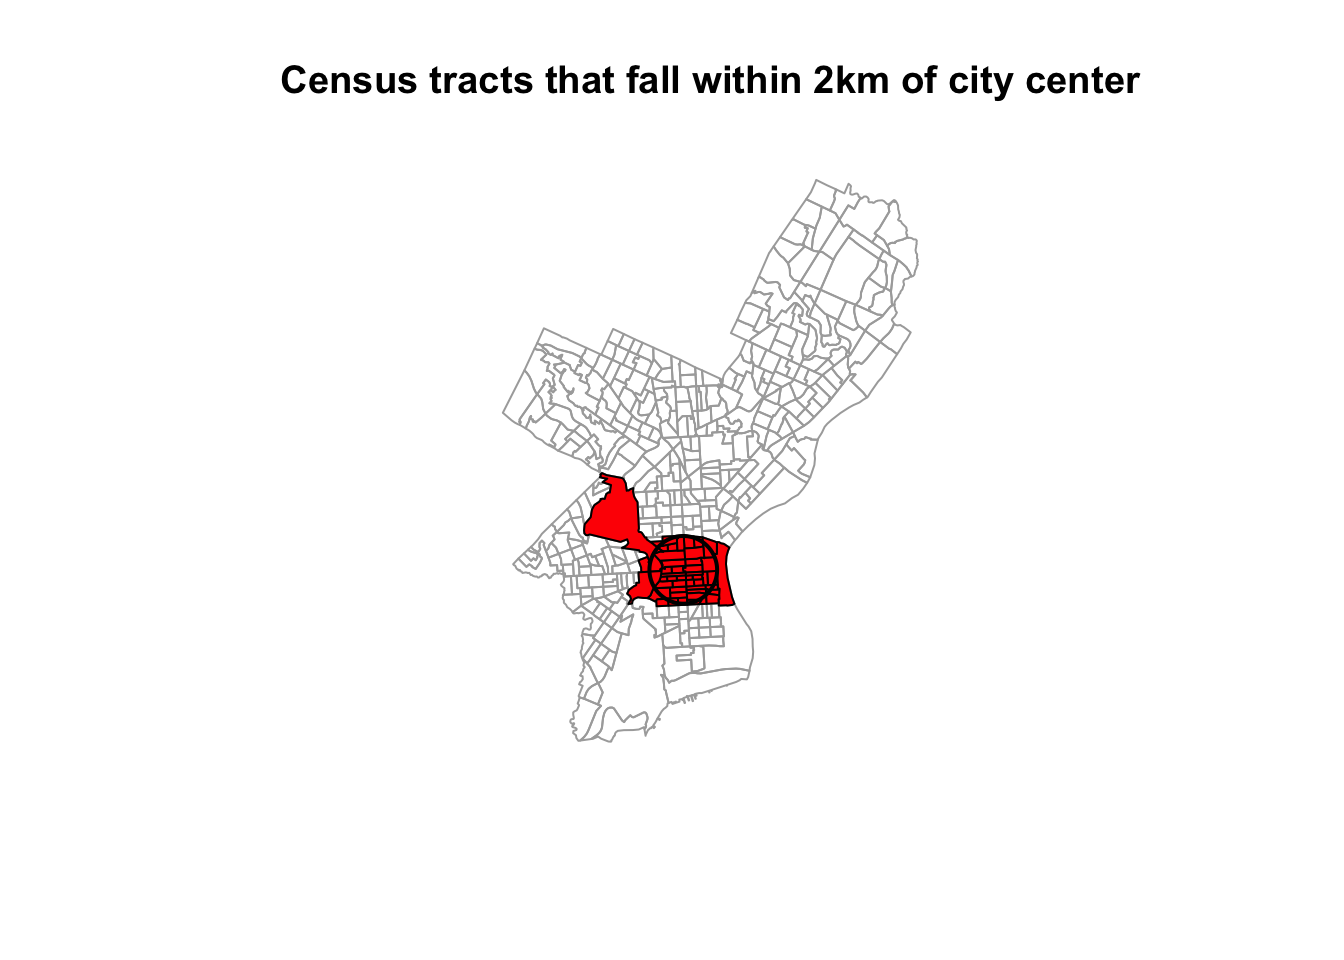
\includegraphics{R-spatial_files/figure-latex/sf-intersection-subset-1.pdf}

\subsection{\texorpdfstring{Using the \texttt{sp}
package}{Using the sp package}}\label{using-the-sp-package}

In order to perform those operations on an \texttt{sp} object we will
need to make use of an additional package, called \texttt{rgeos}. Make
sure you have it loaded.

\begin{Shaded}
\begin{Highlighting}[]
\KeywordTok{library}\NormalTok{(rgeos)}
\CommentTok{# if you need to read it in again}
\CommentTok{# philly_sp <- readOGR("data/Philly/", "PhillyTotalPopHHinc", verbose = F)}
\end{Highlighting}
\end{Shaded}

We will use \texttt{philly\_sp} for the census tract polygons.

Create a \texttt{SpatialPoints} object with the Philadelphia city center
coordinates named \texttt{philly\_ctr\_sp}.

\begin{Shaded}
\begin{Highlighting}[]
\NormalTok{coords <-}\StringTok{ }\KeywordTok{data.frame}\NormalTok{(}\DataTypeTok{x =} \DecValTok{1750160}\NormalTok{, }\DataTypeTok{y =} \FloatTok{467499.9}\NormalTok{) }\CommentTok{# set the coordinates}
\NormalTok{prj <-}\StringTok{ }\KeywordTok{CRS}\NormalTok{(}\StringTok{"+proj=aea +lat_1=29.5 +lat_2=45.5 +lat_0=37.5 +lon_0=-96 +x_0=0 +y_0=0 +datum=NAD83 +units=m +no_defs"}\NormalTok{) }\CommentTok{# the projection string for AEA}
\NormalTok{philly_ctr_sp <-}\StringTok{ }\KeywordTok{SpatialPoints}\NormalTok{(coords, }\DataTypeTok{proj4string =}\NormalTok{ prj) }\CommentTok{# create the spatialPoints}
\end{Highlighting}
\end{Shaded}

Next, we create a buffer around the city center point.\\
Here is where we will use the \texttt{gBuffer()} function from the
\texttt{rgeos} package. For this purpose we will need to provide two
arguments: the \textbf{sp object} and the \textbf{width} of the buffer,
which is assumed to be in map units. The function returns a
\texttt{SpatialPolygons} object to you with the buffer.

\begin{Shaded}
\begin{Highlighting}[]
\NormalTok{philly_buf_sp <-}\StringTok{ }\KeywordTok{gBuffer}\NormalTok{(philly_ctr_sp, }\DataTypeTok{width=}\DecValTok{2000}\NormalTok{)  }\CommentTok{# create buffer around center}
\end{Highlighting}
\end{Shaded}

We will use the \texttt{gIntersects()} function from the \texttt{rgeos}
package to select all census tract polygons that intersect with the
center buffer. The function tests if two geometries (let's name them
\emph{spgeom1} and \emph{spgeom2}) have points in common or not.
\texttt{gIntersects} returns TRUE if \emph{spgeom1} and \emph{spgeom2}
have at least one point in common.

Here is where we determine if the census tracts fall within the buffer.
In addition to our two \texttt{sp} objects (\texttt{philly\_buf} and
\texttt{philly\_sp}) we need to provide one more argument,
\texttt{byid}. It determines if the function should be applied across
ids (TRUE) or the entire object (FALSE) for \emph{spgeom1} and
\emph{spgeom2}. The default setting is FALSE. Since we want to compare
\emph{every single} census tract polygon in our \texttt{philly\_sp}
object we need to set it to TRUE. Then we subset the object with the
census tract polygons.

\begin{Shaded}
\begin{Highlighting}[]
\NormalTok{philly_buf_intersects <-}\StringTok{  }\KeywordTok{gIntersects}\NormalTok{ (philly_buf_sp, philly_sp, }\DataTypeTok{byid=}\OtherTok{TRUE}\NormalTok{) }

\CommentTok{# what kind of object is this?}
\KeywordTok{class}\NormalTok{(philly_buf_intersects)}

\CommentTok{# subset}
\NormalTok{philly_sel_sp <-}\StringTok{ }\NormalTok{philly_sp[}\KeywordTok{as.vector}\NormalTok{(philly_buf_intersects),]}

\CommentTok{# plot}
\KeywordTok{plot}\NormalTok{ (philly_sp, }\DataTypeTok{border=}\StringTok{"#aaaaaa"}\NormalTok{)}
\KeywordTok{plot}\NormalTok{ (philly_sel_sp, }\DataTypeTok{add=}\NormalTok{T, }\DataTypeTok{col=}\StringTok{"red"}\NormalTok{) }
\KeywordTok{plot}\NormalTok{ (philly_buf_sp, }\DataTypeTok{add=}\NormalTok{T, }\DataTypeTok{lwd =} \DecValTok{2}\NormalTok{)}
\end{Highlighting}
\end{Shaded}

\section{Reprojecting}\label{reprojecting}

Occasionally you may have to change the coordinates of your spatial
object into a new Coordinate Reference System (CRS). Functions to
transform, or \emph{reproject} spatial objects typically take the
following two arguments:

\begin{itemize}
\tightlist
\item
  the spatial object to reproject
\item
  a CRS object with the new projection definition
\end{itemize}

You can reproject

\begin{itemize}
\tightlist
\item
  a \texttt{sf} object with \texttt{st\_transform()}\\
\item
  a \texttt{Spatial*} object with \texttt{spTransform()}\\
\item
  a \texttt{raster} object with \texttt{projectRaster()}
\end{itemize}

The perhaps trickiest part here is to determine the definition of the
projection, which needs to be a character string in
\href{http://trac.osgeo.org/proj/}{proj4} format. You can
\href{http://www.spatialreference.org}{look it up online}. For example
for \href{http://spatialreference.org/ref/epsg/wgs-84-utm-zone-33n/}{UTM
zone 33N (EPSG:32633)} the string would be:

\href{http://spatialreference.org/ref/epsg/wgs-84-utm-zone-33n/proj4js/}{\texttt{+proj=utm\ +zone=33\ +ellps=WGS84\ +datum=WGS84\ +units=m\ +no\_defs}}

You can retrieve the CRS:

\begin{itemize}
\tightlist
\item
  from an \texttt{sf} object with \texttt{st\_crs()}
\item
  from an existing \texttt{Spatial*} object with \texttt{proj4string()}
\item
  from a \texttt{raster} object with \texttt{crs()}
\end{itemize}

Let us go back to the \texttt{"PhillyHomicides"} shapefile we exported
earlier. Let's read it back in and reproject it so it matches the
projection of the Philadelphia Census tracts.

Now let us check the CRS for both files.

\begin{Shaded}
\begin{Highlighting}[]
\CommentTok{#If you need to read the file back in:}
\CommentTok{#philly_homicides_sf <- st_read("data/PhillyHomicides/")}

\KeywordTok{st_crs}\NormalTok{(philly_sf)}
\end{Highlighting}
\end{Shaded}

\begin{verbatim}
#> Coordinate Reference System:
#>   EPSG: 102003 
#>   proj4string: "+proj=aea +lat_1=29.5 +lat_2=45.5 +lat_0=37.5 +lon_0=-96 +x_0=0 +y_0=0 +datum=NAD83 +units=m +no_defs"
\end{verbatim}

\begin{Shaded}
\begin{Highlighting}[]
\KeywordTok{st_crs}\NormalTok{(philly_homicides_sf)}
\end{Highlighting}
\end{Shaded}

\begin{verbatim}
#> Coordinate Reference System:
#>   EPSG: 4326 
#>   proj4string: "+proj=longlat +datum=WGS84 +no_defs"
\end{verbatim}

We see that the CRS are different: we have \texttt{+proj=aea...} and
\texttt{+proj=longlat...}. AEA refers to
\href{http://spatialreference.org/ref/esri/102003/}{USA Contiguous
Albers Equal Area Conic} which is a projected coordinate system with
numeric units. We will need this below for our spatial operations, so we
will make sure both files are in that same CRS.

We use \texttt{st\_transform} and assign the result to a new object.
Note how we also use \texttt{str\_crs} to extract the projection
defitition from \texttt{philly\_sf}, so we don't have to type it out.

\begin{Shaded}
\begin{Highlighting}[]
\NormalTok{philly_homicides_sf_aea <-}\StringTok{ }\KeywordTok{st_transform}\NormalTok{(philly_homicides_sf, }\KeywordTok{st_crs}\NormalTok{(philly_sf))}
\end{Highlighting}
\end{Shaded}

We can use the \texttt{range()} command from the R base package to
compare the coordinates before and after reprojection and confirm that
we actually have transformed them. \texttt{range()} returns the
\emph{min} and \emph{max} value of a vector of numbers.

\begin{Shaded}
\begin{Highlighting}[]
\KeywordTok{range}\NormalTok{(}\KeywordTok{st_coordinates}\NormalTok{(philly_homicides_sf))}
\end{Highlighting}
\end{Shaded}

\begin{verbatim}
#> [1] -75.26809  40.13086
\end{verbatim}

\begin{Shaded}
\begin{Highlighting}[]
\KeywordTok{range}\NormalTok{(}\KeywordTok{st_coordinates}\NormalTok{(philly_homicides_sf_aea))}
\end{Highlighting}
\end{Shaded}

\begin{verbatim}
#> [1]  457489.7 1763671.8
\end{verbatim}

We can also compare them visually with:

\begin{Shaded}
\begin{Highlighting}[]
\KeywordTok{par}\NormalTok{(}\DataTypeTok{mfrow=}\KeywordTok{c}\NormalTok{(}\DecValTok{1}\NormalTok{,}\DecValTok{2}\NormalTok{)) }
\KeywordTok{plot}\NormalTok{(}\KeywordTok{st_geometry}\NormalTok{(philly_homicides_sf), }\DataTypeTok{axes=}\OtherTok{TRUE}\NormalTok{, }\DataTypeTok{main =} \StringTok{"before transform - latlon"}\NormalTok{)}
\KeywordTok{plot}\NormalTok{(}\KeywordTok{st_geometry}\NormalTok{(philly_homicides_sf_aea), }\DataTypeTok{axes=}\OtherTok{TRUE}\NormalTok{, }\DataTypeTok{main =} \StringTok{"after transform - aea"}\NormalTok{)}
\end{Highlighting}
\end{Shaded}

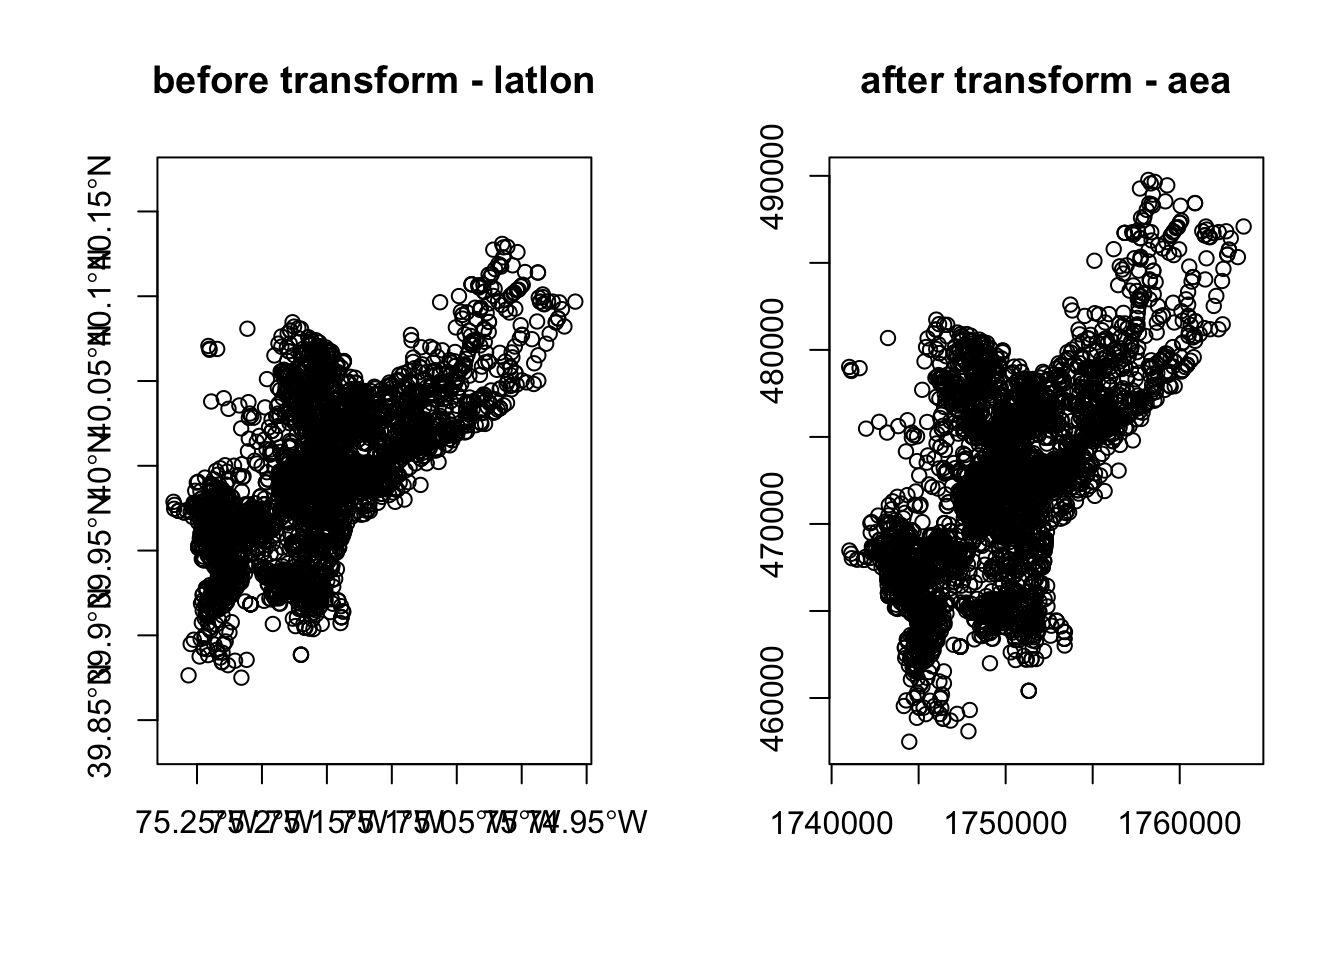
\includegraphics{R-spatial_files/figure-latex/compare-reproj-plots-sf-1.pdf}

Lastly, let us save the reprojected file as
\texttt{PhillyHomicides\_aea} shapefile, as we will use it later on.

\begin{Shaded}
\begin{Highlighting}[]
\KeywordTok{st_write}\NormalTok{(philly_homicides_sf_aea, }\StringTok{"data/PhillyHomicides_aea"}\NormalTok{, }\DataTypeTok{driver =} \StringTok{"ESRI Shapefile"}\NormalTok{)}
\end{Highlighting}
\end{Shaded}

\subsection{\texorpdfstring{For \texttt{sp}}{For sp}}\label{for-sp}

Below is the equivalent for \texttt{sp} objects. This is very similar,
except that we wrap the \texttt{CRS} function ariound the result of
\texttt{proj4string}, because \texttt{spTransform} requires a CRS
object.

\begin{Shaded}
\begin{Highlighting}[]
\NormalTok{ph_homic_sp <-}\StringTok{ }\KeywordTok{readOGR}\NormalTok{(}\StringTok{"data/PhillyHomicides/"}\NormalTok{, }\StringTok{"PhillyHomicides"}\NormalTok{)}
\KeywordTok{proj4string}\NormalTok{(philly_sp)}
\KeywordTok{proj4string}\NormalTok{(philly_homicides_sp)}
\NormalTok{philly_homicides_sp_aea <-}\StringTok{ }\KeywordTok{spTransform}\NormalTok{(philly_homicides_sp, }\KeywordTok{CRS}\NormalTok{(}\KeywordTok{proj4string}\NormalTok{(philly_sp)))}

\NormalTok{## check the coordinates ##}
\KeywordTok{range}\NormalTok{(}\KeywordTok{coordinates}\NormalTok{(ph_homic_aea_sp))}
\KeywordTok{range}\NormalTok{(}\KeywordTok{coordinates}\NormalTok{(ph_homic_sp))}

\NormalTok{## write out}
\KeywordTok{writeOGR}\NormalTok{(philly_homicides_sp_aea, }\StringTok{"data/PhillyHomicides_AEA"}\NormalTok{, }\StringTok{"PhillyHomcides_AEA"}\NormalTok{, }\DataTypeTok{driver =} \StringTok{"ESRI Shapefile"}\NormalTok{)}
\end{Highlighting}
\end{Shaded}

\subsection{Raster reprojection}\label{raster-reprojection}

Here is what it would look like to reproject the HARV raster used
earlier to a WGS84 projection. We see that the original projection is in
UTM.

\begin{Shaded}
\begin{Highlighting}[]
\CommentTok{# if you need to load again:}
\CommentTok{#HARV <- raster("data/HARV_RGB_Ortho.tif")}
\KeywordTok{crs}\NormalTok{(HARV)}
\end{Highlighting}
\end{Shaded}

\begin{verbatim}
#> CRS arguments:
#>  +proj=utm +zone=18 +datum=WGS84 +units=m +no_defs +ellps=WGS84
#> +towgs84=0,0,0
\end{verbatim}

\begin{Shaded}
\begin{Highlighting}[]
\NormalTok{HARV_WGS84 <-}\StringTok{ }\KeywordTok{projectRaster}\NormalTok{(HARV, }\DataTypeTok{crs=}\StringTok{"+init=epsg:4326"}\NormalTok{)}
\end{Highlighting}
\end{Shaded}

Let's look at the coordinates to see the effect:

\begin{Shaded}
\begin{Highlighting}[]
\KeywordTok{extent}\NormalTok{(HARV)}
\end{Highlighting}
\end{Shaded}

\begin{verbatim}
#> class       : Extent 
#> xmin        : 731998.5 
#> xmax        : 732766.8 
#> ymin        : 4712956 
#> ymax        : 4713536
\end{verbatim}

\begin{Shaded}
\begin{Highlighting}[]
\KeywordTok{extent}\NormalTok{(HARV_WGS84)}
\end{Highlighting}
\end{Shaded}

\begin{verbatim}
#> class       : Extent 
#> xmin        : -72.17505 
#> xmax        : -72.16544 
#> ymin        : 42.53393 
#> ymax        : 42.5394
\end{verbatim}

\begin{Shaded}
\begin{Highlighting}[]
\KeywordTok{ncell}\NormalTok{(HARV)}
\end{Highlighting}
\end{Shaded}

\begin{verbatim}
#> [1] 7120141
\end{verbatim}

\begin{Shaded}
\begin{Highlighting}[]
\KeywordTok{ncell}\NormalTok{(HARV_WGS84)}
\end{Highlighting}
\end{Shaded}

\begin{verbatim}
#> [1] 7687552
\end{verbatim}

And here is the visual proof:

\begin{Shaded}
\begin{Highlighting}[]
\KeywordTok{plot}\NormalTok{(HARV, }\DataTypeTok{main =} \StringTok{"before transform - UTM"}\NormalTok{)}
\end{Highlighting}
\end{Shaded}

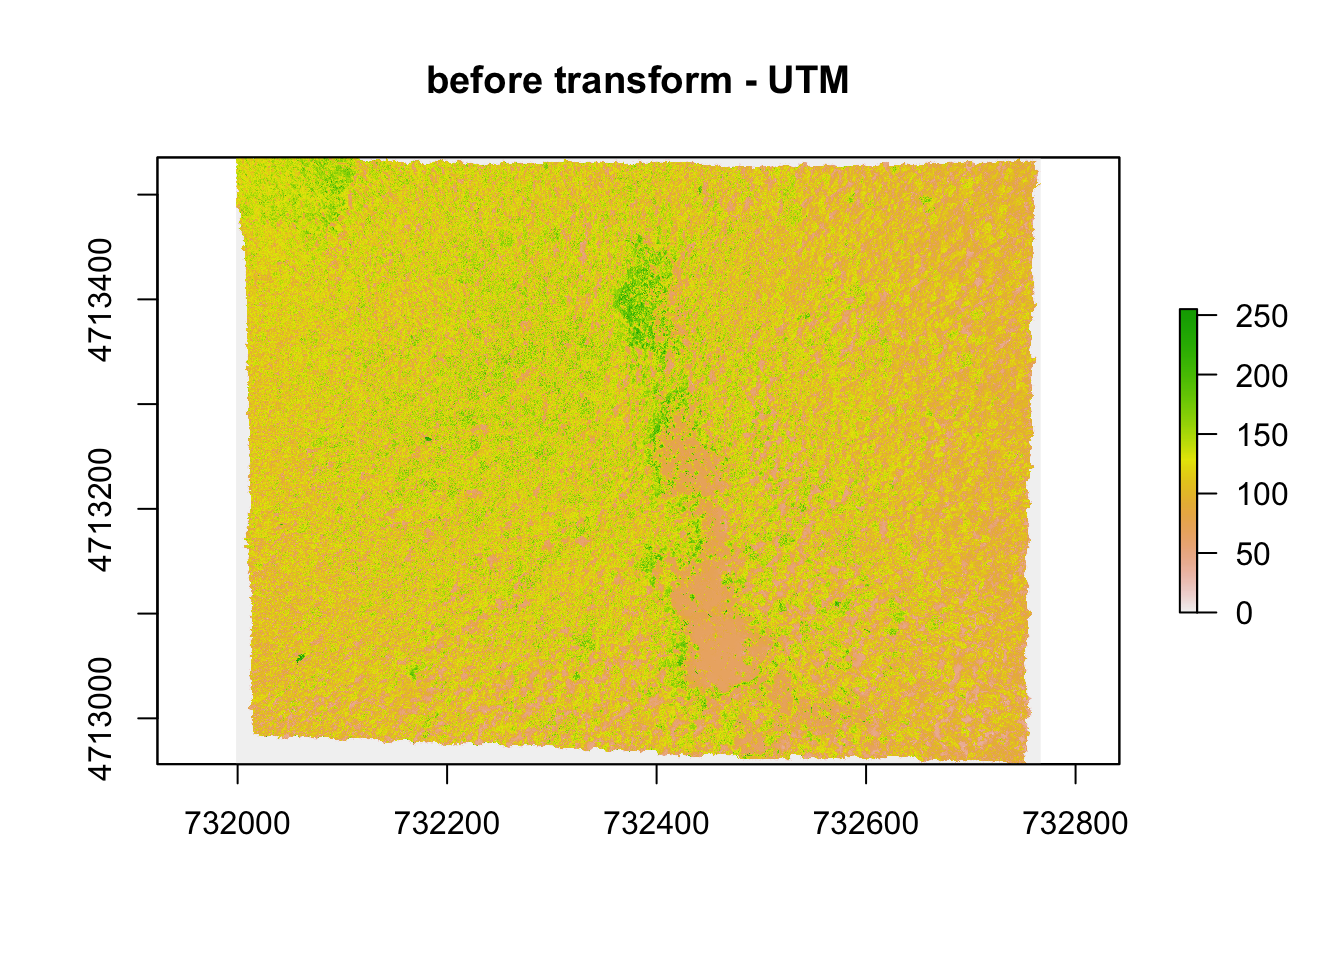
\includegraphics{R-spatial_files/figure-latex/raster-reproject-plot1-1.pdf}

\begin{Shaded}
\begin{Highlighting}[]
\KeywordTok{plot}\NormalTok{(HARV_WGS84, }\DataTypeTok{main =} \StringTok{"after transform - WGS84"}\NormalTok{)}
\end{Highlighting}
\end{Shaded}

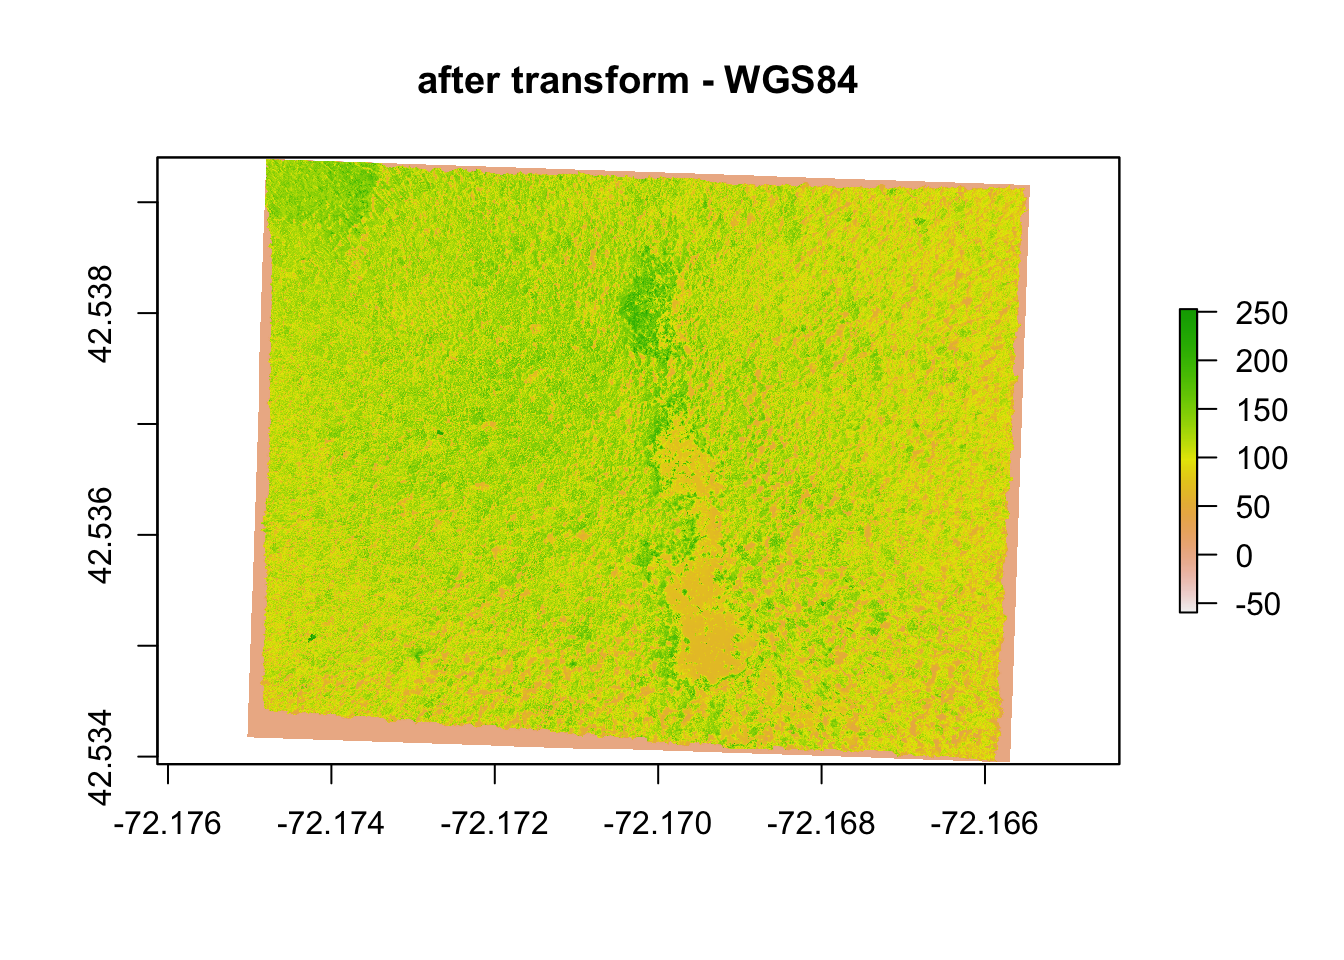
\includegraphics{R-spatial_files/figure-latex/raster-reproject-plot2-1.pdf}

\section{Spatial Aggregation: Points in
Polygons}\label{spatial-aggregation-points-in-polygons}

Now that we have both homicides and census tracts in the same projection
we will forge ahead and ask for the density of homicides for
\textbf{each census tract} in Philadelphia: \(\frac{{homicides}}{area}\)

To achieve this this we join the points of homicide incidence to the
census tract polygon and count them up for each polygon. You might be
familiar with this operation from other GIS packages.

\subsection{\texorpdfstring{With \texttt{sf}}{With sf}}\label{with-sf-1}

We will use piping and build up our object in the following way. First
we calculate the area for each tract. We use the \texttt{st\_area}
function on the geometry column and add the result.

\begin{Shaded}
\begin{Highlighting}[]
\NormalTok{philly_sf }\OperatorTok\StringTok{ }
\StringTok{  }\KeywordTok{mutate}\NormalTok{(}\DataTypeTok{tract_area =} \KeywordTok{st_area}\NormalTok{(geometry)) }\OperatorTok\StringTok{ }
\StringTok{  }\KeywordTok{head}\NormalTok{()}
\end{Highlighting}
\end{Shaded}

Next, we use st\_join to perform a spatial join with the points:

\begin{Shaded}
\begin{Highlighting}[]
\NormalTok{philly_sf }\OperatorTok\StringTok{ }
\StringTok{  }\KeywordTok{mutate}\NormalTok{(}\DataTypeTok{tract_area =} \KeywordTok{st_area}\NormalTok{(geometry)) }\OperatorTok\StringTok{ }
\StringTok{  }\KeywordTok{st_join}\NormalTok{(philly_homicides_sf_aea) }\OperatorTok
\StringTok{  }\KeywordTok{head}\NormalTok{()}
\end{Highlighting}
\end{Shaded}

Now we can group by a variable that uiquely identifies the census
tracts, (we choose \emph{GEOID10}) and use \texttt{summarize} to count
the points for each tract and calculate the homicide rate. Since our
units are in sq meter. multiply by by 1000000 to get sq km. We also need
to carry over the area, which I do using \texttt{unique}.

We also assign the output to a new object \texttt{crime\_rate}.

\begin{Shaded}
\begin{Highlighting}[]
\NormalTok{crime_rate <-}\StringTok{ }\NormalTok{philly_sf }\OperatorTok\StringTok{ }
\StringTok{      }\KeywordTok{mutate}\NormalTok{(}\DataTypeTok{tract_area =} \KeywordTok{st_area}\NormalTok{(geometry)) }\OperatorTok
\StringTok{      }\KeywordTok{st_join}\NormalTok{(philly_homicides_sf_aea) }\OperatorTok
\StringTok{      }\KeywordTok{group_by}\NormalTok{(GEOID10) }\OperatorTok\StringTok{ }
\StringTok{      }\KeywordTok{summarize}\NormalTok{(}\DataTypeTok{n_homic =} \KeywordTok{n}\NormalTok{(),}
                \DataTypeTok{tract_area =} \KeywordTok{unique}\NormalTok{(tract_area),}
                \DataTypeTok{homic_rate =}\NormalTok{ n_homic}\OperatorTok{/}\NormalTok{tract_area }\OperatorTok{*}\StringTok{ }\FloatTok{1e6}\NormalTok{) }
\end{Highlighting}
\end{Shaded}

And here is a simple plot:

\begin{Shaded}
\begin{Highlighting}[]
\KeywordTok{plot}\NormalTok{(crime_rate[}\StringTok{"homic_rate"}\NormalTok{])}
\end{Highlighting}
\end{Shaded}

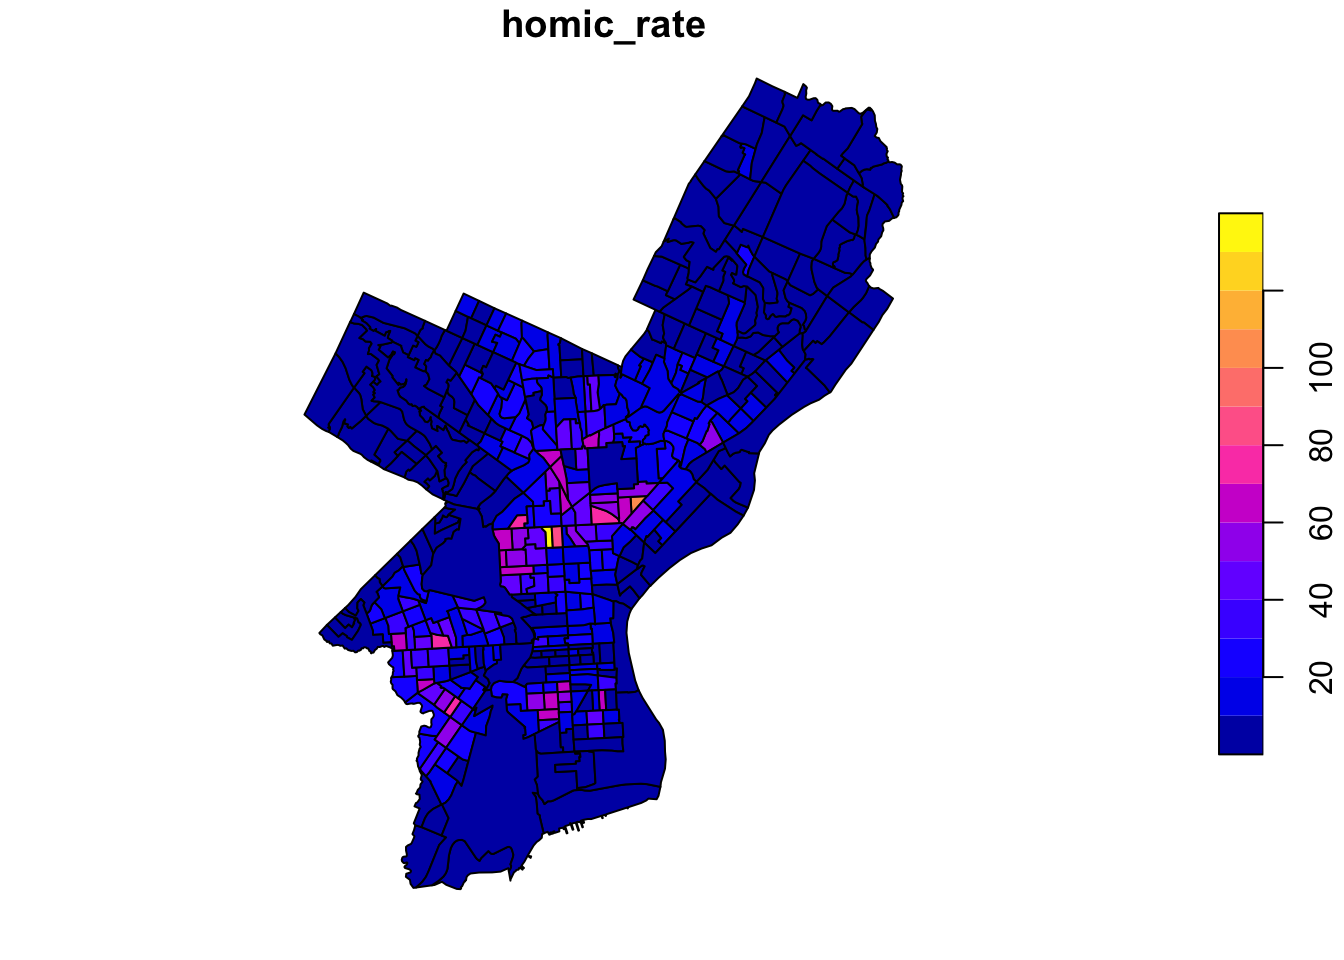
\includegraphics{R-spatial_files/figure-latex/sf-hom-ratio-plot-1.pdf}

Finally, we write this out for later:

\begin{Shaded}
\begin{Highlighting}[]
\KeywordTok{st_write}\NormalTok{(crime_rate, }\StringTok{"data/PhillyCrimerate"}\NormalTok{, }\DataTypeTok{driver =} \StringTok{"ESRI Shapefile"}\NormalTok{)}
\end{Highlighting}
\end{Shaded}

\subsection{\texorpdfstring{With \texttt{sp}}{With sp}}\label{with-sp-1}

For \texttt{sp} objects we can use the \texttt{aggregate()}
function\footnote{There is also an \texttt{aggregate()} function in the
  \texttt{stats} package that comes with the R standard install. Note
  that \texttt{sp} extends this function so it can take
  \texttt{Spatial*} objects and aggregate over the geometric features.}.
Here are the arguments that it needs:

\begin{itemize}
\tightlist
\item
  the \texttt{SpatialPointDataframe}with the homicide incidents as point
  locations,
\item
  the \texttt{SpatialPolygonDataframe} with the census tract polygons to
  aggregate on, and
\item
  an aggregate function. Since we are interested in counting the points
  (i.e.~the rows of all the points that belong to a certain polygon), we
  can use length (of the respective vectors of the aggregated data).
\end{itemize}

To count homicides per census tract we can use any field from
\texttt{ph\_homic\_aea} for homicide incidents (we chose
\texttt{OBJ\_ID}) and \texttt{philly} polygons to aggregate on and save
the result as \texttt{ph\_hom\_count}. Use \texttt{length} as aggregate
function.

\begin{Shaded}
\begin{Highlighting}[]
\NormalTok{ph_hom_count_sp <-}\StringTok{ }\KeywordTok{aggregate}\NormalTok{(}\DataTypeTok{x =}\NormalTok{ ph_homic_aea_sp[}\StringTok{"OBJ_ID"}\NormalTok{], }\DataTypeTok{by =}\NormalTok{ philly_sp, }\DataTypeTok{FUN =}\NormalTok{ length)}
\CommentTok{# make sure we understand this error message:}
\CommentTok{# aggregate(x = ph_homic_sp, by = philly_sp, FUN = length) }
\end{Highlighting}
\end{Shaded}

Now let us investigate the object we created.

\begin{Shaded}
\begin{Highlighting}[]
\KeywordTok{class}\NormalTok{(ph_hom_count_sp)}
\KeywordTok{names}\NormalTok{(ph_hom_count_sp)}
\KeywordTok{head}\NormalTok{(ph_hom_count_sp)}
\end{Highlighting}
\end{Shaded}

Now we can calculate the density of homicides in Philadelphia,
normalized over the area for each census tract.

We use \texttt{gArea()} from the \texttt{rgeos} library. \texttt{gArea},
when given a \texttt{SpatialPolygon}, calculates the size of the area
covered. If we need that calculation for each polygon, we set
\texttt{byid\ =\ TRUE}. Units are in map units.

\begin{Shaded}
\begin{Highlighting}[]
\KeywordTok{library}\NormalTok{(rgeos)}
\CommentTok{# we multiply by by 1000000 to get sq km.}
\NormalTok{ph_hom_count_sp}\OperatorTok{$}\NormalTok{homic_dens <-}\StringTok{ }\FloatTok{1e6} \OperatorTok{*}\StringTok{ }\NormalTok{(ph_hom_count_sp}\OperatorTok{$}\NormalTok{OBJ_ID}\OperatorTok{/}\KeywordTok{gArea}\NormalTok{(ph_hom_count_sp, }\DataTypeTok{byid =} \OtherTok{FALSE}\NormalTok{))}

\KeywordTok{hist}\NormalTok{(ph_hom_count_sp}\OperatorTok{$}\NormalTok{homic_dens)}
\end{Highlighting}
\end{Shaded}

We will write it out for later. (Note that this will produce an error if
the file already exists. You can force it to write out with the option
\texttt{overwrite\_layer\ =\ TRUE})

\begin{Shaded}
\begin{Highlighting}[]
\KeywordTok{writeOGR}\NormalTok{(ph_hom_count_sp, }\StringTok{"data/PhillyCrimerate"}\NormalTok{, }\StringTok{"PhillyCrimerate"}\NormalTok{, }\DataTypeTok{driver =} \StringTok{"ESRI Shapefile"}\NormalTok{)}
\end{Highlighting}
\end{Shaded}

There might be other instances where we don't want to aggregate, but
might only want to know which polygon a point falls into. In that case
we can use \texttt{over()}. In fact, the \texttt{aggregate()} function
used above makes use of \texttt{over()}. See
\url{https://cran.r-project.org/web/packages/sp/vignettes/over.pdf} for
more details on the over-methods. \texttt{point.in.poly()} from the
\href{https://cran.r-project.org/package=spatialEco}{\texttt{spatialEco}}
package intersects point and polygons and adds polygon attributes to
points. There is also \texttt{point.in.polygon()} from the \texttt{sp}
package which tests if a point or set of points fall in a given polygon.

\subsection{\texorpdfstring{\texttt{sp} - \texttt{sf}
comparison}{sp - sf comparison}}\label{sp---sf-comparison}

\begin{longtable}[]{@{}lll@{}}
\toprule
how to.. & for \texttt{sp} objects & for \texttt{sf}
objects\tabularnewline
\midrule
\endhead
join attributes & \texttt{sp::merge()} & \texttt{dplyr::*\_join()} (also
\texttt{sf::merge()})\tabularnewline
reproject & \texttt{spTransform()} &
\texttt{st\_transform()}\tabularnewline
retrieve (or assign) CRS & \texttt{proj4string()} &
\texttt{st\_crs()}\tabularnewline
count points in polygons & \texttt{over()} & \texttt{st\_within} and
\texttt{aggregate()}\tabularnewline
buffer & \texttt{rgeos::gBuffer()} (separate package) &
\texttt{st\_buffer()}\tabularnewline
select by location &
\href{https://www.rdocumentation.org/packages/rgeos/}{\texttt{g*}
functions} from \texttt{rgeos} &
\href{https://www.rdocumentation.org/packages/sf/topics/geos}{st\_* geos
functions} in \texttt{sf}\tabularnewline
\bottomrule
\end{longtable}

Here are some additional packages that use vector data:

\begin{itemize}
\tightlist
\item
  \href{https://CRAN.R-project.org/package=stplanr}{\texttt{stplanr}}:
  Functionality and data access tools for transport planning, including
  origin-destination analysis, route allocation and modelling travel
  patterns.
\item
  \href{https://CRAN.R-project.org/package=bikedata}{\texttt{bikedata}}:
  Data from public hire bicycle systems,including London, New York,
  Chicago, Washington DC, Boston, Los Angeles, and Philadelphia
\end{itemize}

\section{\texorpdfstring{\texttt{raster}
operations}{raster operations}}\label{raster-operations}

\begin{quote}
\begin{quote}
\begin{quote}
to come
\end{quote}
\end{quote}
\end{quote}

Some helpful packages that deal with raster data:

\begin{itemize}
\tightlist
\item
  \href{https://CRAN.R-project.org/package=landscapetools}{\texttt{landscapetools}}
  provides utility functions to complete tasks involved in common
  landscape analysis.
\item
  \href{https://CRAN.R-project.org/package=getlandsat}{\texttt{getlandsat}}:
  Get Landsat 8 Data from
  \href{https://registry.opendata.aws/landsat-8/}{Amazon Public Data
  Sets}
\item
  \href{https://CRAN.R-project.org/package=MODIStsp}{\texttt{MODIStsp}}:
  automates the creation of time series of rasters derived from MODIS
  Land Products data
\item
  \href{https://cran.r-project.org/package=FedData}{\texttt{FedData}}:
  Download geospatial Data from federated data sources, including the
  The National Elevation Dataset digital elevation models, the Global
  Historical Climatology Network, the National Land Cover Database, and
  more.
\end{itemize}

\chapter{Making Maps in R}\label{mapping}

\begin{quote}
Learning Objectives

\begin{itemize}
\tightlist
\item
  plot an \texttt{sf} object
\item
  create a choropleth map with \texttt{ggplot}
\item
  add a basemap with \texttt{ggmap}
\item
  use \texttt{RColorBrewer} to improve legend colors
\item
  use \texttt{classInt}to improve legend breaks
\item
  create a choropleth map with \texttt{tmap}
\item
  create an interactive map with \texttt{leaflet}
\item
  customize a \texttt{leaflet} map with popups and layer controls
\end{itemize}
\end{quote}

\begin{center}\rule{0.5\linewidth}{\linethickness}\end{center}

In the preceding examples we have used the base \texttt{plot} command to
take a quick look at our spatial objects.

In this section we will explore several alternatives to map spatial data
with R. For more packages see the ``Visualisation'' section of the
\href{https://cran.r-project.org/web/views/Spatial.html}{CRAN Task
View}.

Mapping packages are in the process of keeping up with the development
of the new \texttt{sf} package, so they typicall accept both \texttt{sp}
and \texttt{sf} objects. However, there are a few exceptions.

Of the packages shown here \texttt{spplot()}, which is part of the good
old \texttt{sp} package, only takes \texttt{sp} objects. The
\href{https://github.com/tidyverse/ggplot2/releases}{development version
of \texttt{ggplot2}} can take \texttt{sf} objects, though \texttt{ggmap}
\href{https://github.com/tidyverse/ggplot2/issues/2130}{seems to still
have issues} with \texttt{sf}. Both \texttt{tmap} and \texttt{leaflet}
can also handle both \texttt{sp} and \texttt{sf} objects.

\section{\texorpdfstring{Plotting simple features (\texttt{sf}) with
\texttt{plot}}{Plotting simple features (sf) with plot}}\label{plotting-simple-features-sf-with-plot}

As we have already briefly seen, the \texttt{sf} package extends the
base \texttt{plot} command, so it can be used on \texttt{sf} objects. If
used without any arguments it will plot all the attributes.

\begin{Shaded}
\begin{Highlighting}[]
\NormalTok{philly_crimes_sf <-}\StringTok{  }\KeywordTok{st_read}\NormalTok{(}\StringTok{"data/PhillyCrimerate/"}\NormalTok{, }\DataTypeTok{quiet =} \OtherTok{TRUE}\NormalTok{)}
\KeywordTok{plot}\NormalTok{(philly_crimes_sf)}
\end{Highlighting}
\end{Shaded}

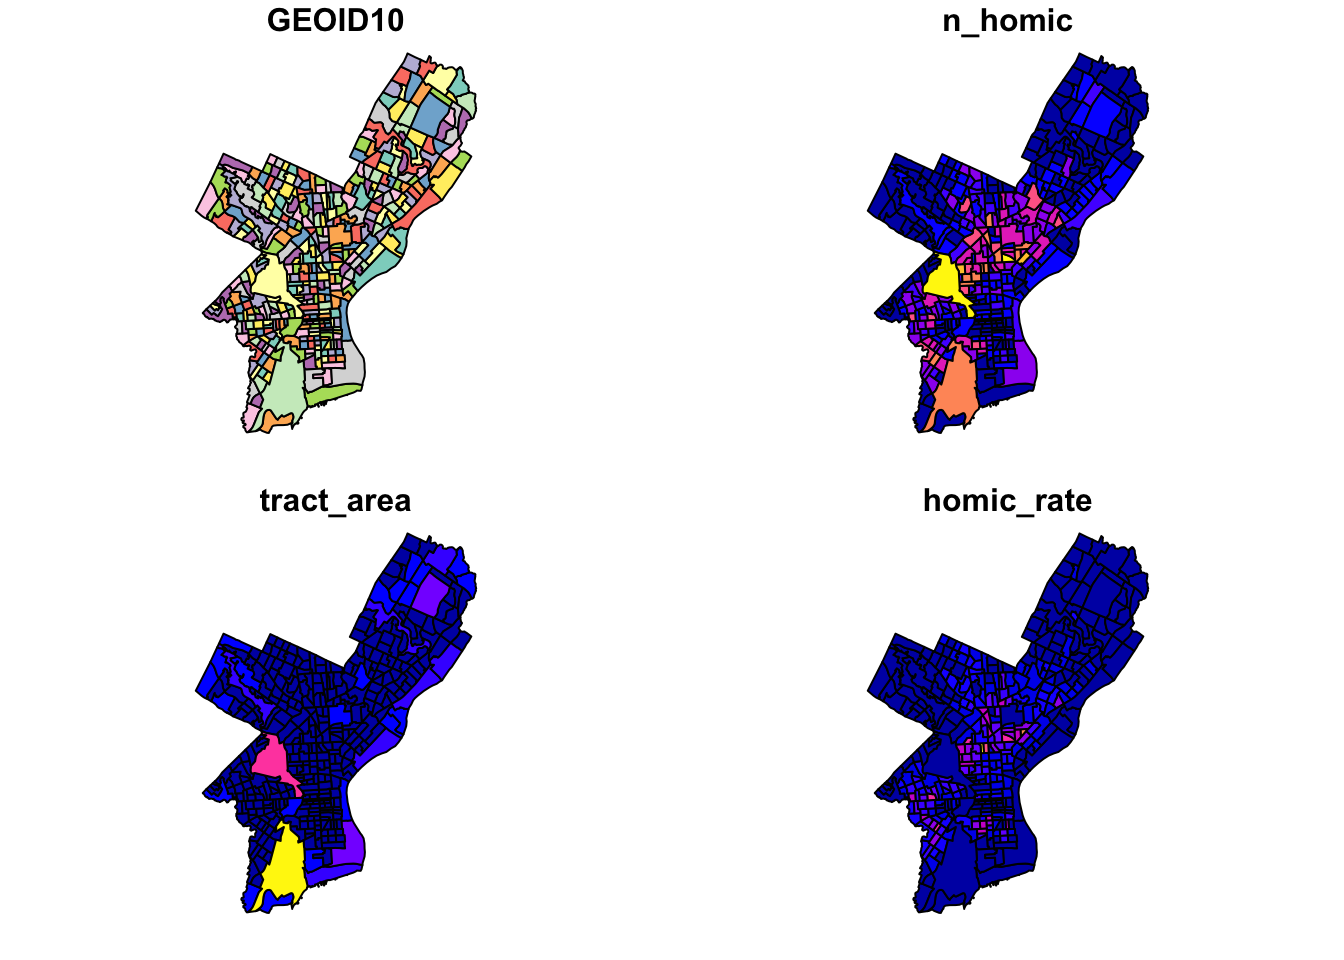
\includegraphics{R-spatial_files/figure-latex/sf-plot-default-1.pdf}

To plot a single attribute we need to provide an object of class
\texttt{sf}, like so:

\begin{Shaded}
\begin{Highlighting}[]
\KeywordTok{plot}\NormalTok{(philly_crimes_sf}\OperatorTok{$}\NormalTok{homic_rate) }\CommentTok{# this is a numeric vector!}
\end{Highlighting}
\end{Shaded}

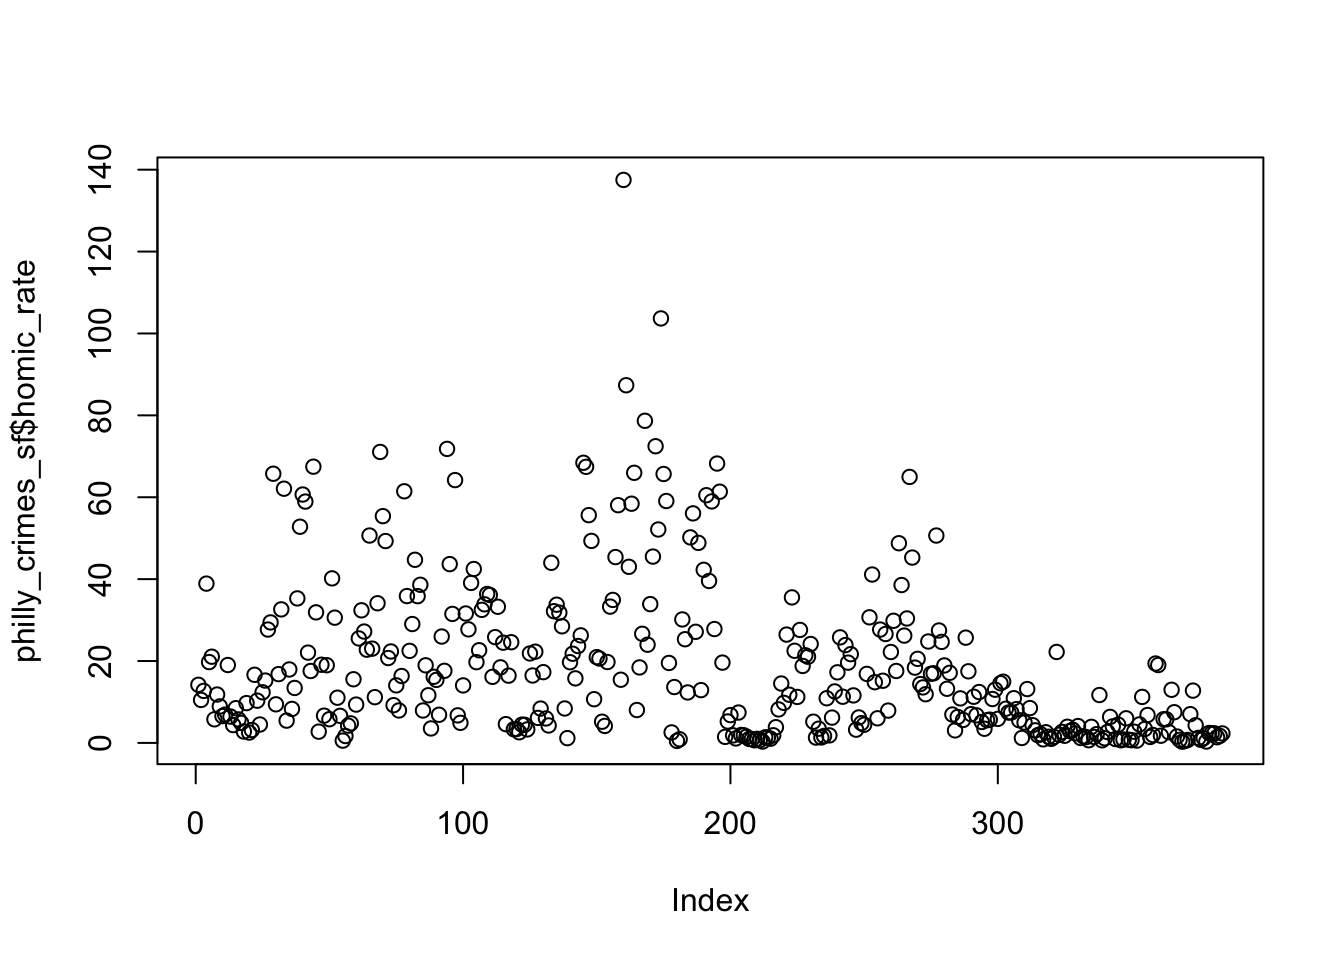
\includegraphics{R-spatial_files/figure-latex/sf-plot-single-1.pdf}

\begin{Shaded}
\begin{Highlighting}[]
\KeywordTok{plot}\NormalTok{(philly_crimes_sf[}\StringTok{"homic_rate"}\NormalTok{])}
\end{Highlighting}
\end{Shaded}

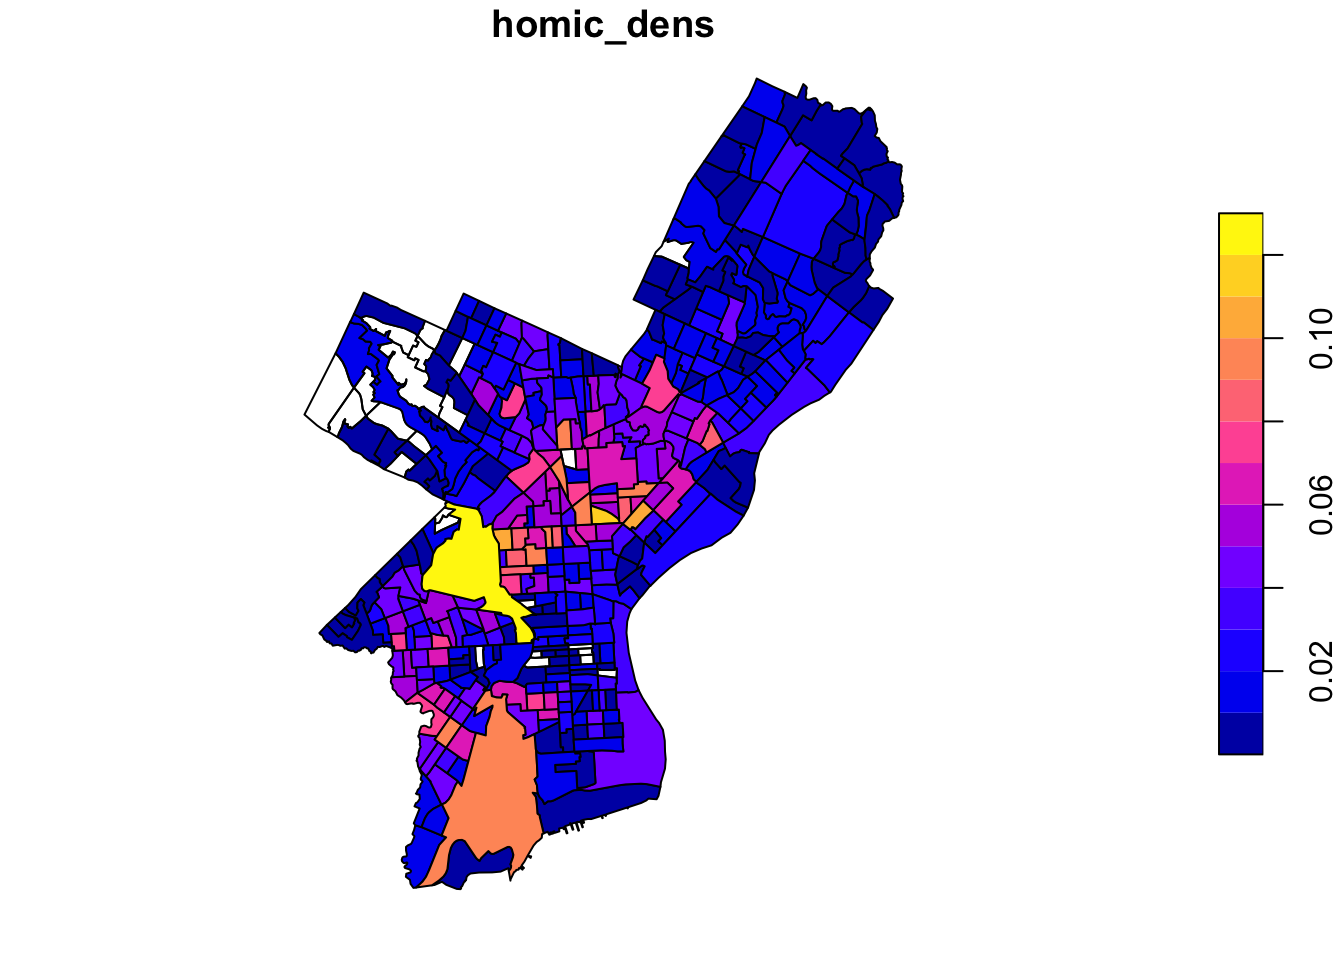
\includegraphics{R-spatial_files/figure-latex/sf-plot-single-2.pdf}

Since our values are unevenly distributed\ldots{}:

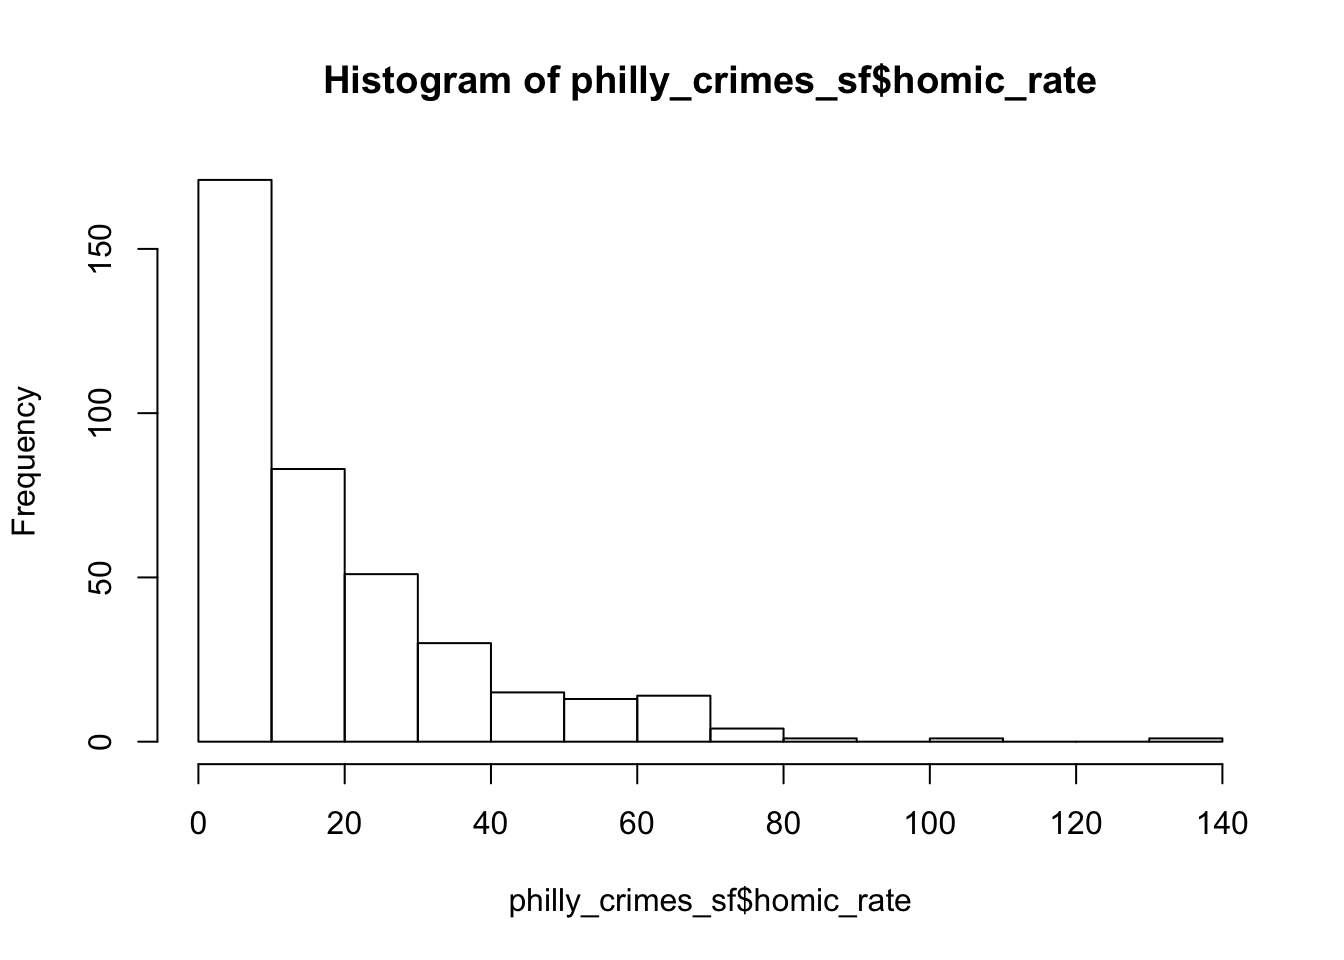
\includegraphics{R-spatial_files/figure-latex/unnamed-chunk-12-1.pdf}

\ldots{}we might want to set the breaks to quantiles in order to better
distinguish the census tracts with low values. This can be done by using
the \texttt{breaks} argument for the sf plot function.

\begin{Shaded}
\begin{Highlighting}[]
\KeywordTok{plot}\NormalTok{(philly_crimes_sf[}\StringTok{"homic_rate"}\NormalTok{], }
     \DataTypeTok{main =} \StringTok{"Philadelphia homicide density per square km"}\NormalTok{, }
     \DataTypeTok{breaks =} \StringTok{"quantile"}\NormalTok{)}
\end{Highlighting}
\end{Shaded}

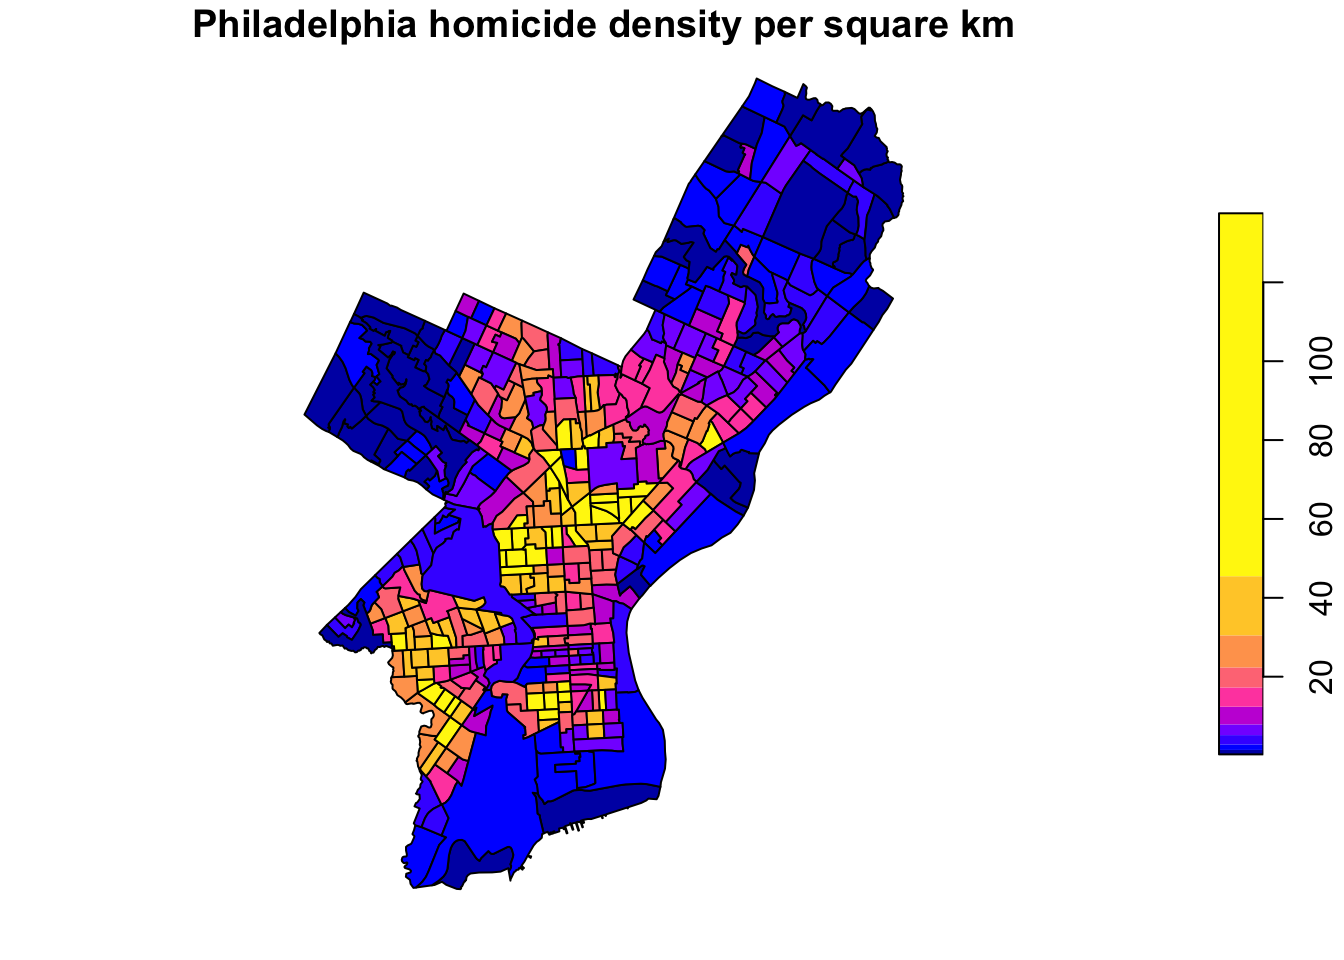
\includegraphics{R-spatial_files/figure-latex/sf-plot-qantile-1.pdf}

We can change the color palette using a library called
\texttt{RColorBrewer}\footnote{This is not the only way to provide color
  palettes. You can create your customized palette in many different
  ways or simply as a vector of hexbin color codes, like
  \texttt{c(\ "\#FDBB84"\ "\#FC8D59"\ "\#EF6548")}.}. For more about
ColorBrewer palettes read \href{http://colorbrewer2.org}{this}.

To make the color palettes from ColorBrewer available as R palettes we
use the \texttt{brewer.pal()} function. It takes two arguments: - the
number of different colors desired and - the name of the palette as
character string.

We select 7 colors from the `Orange-Red' plaette and assign it to an
object \texttt{pal}.

\begin{Shaded}
\begin{Highlighting}[]
\KeywordTok{library}\NormalTok{(RColorBrewer)}
\NormalTok{pal <-}\StringTok{ }\KeywordTok{brewer.pal}\NormalTok{(}\DecValTok{7}\NormalTok{, }\StringTok{"OrRd"}\NormalTok{) }\CommentTok{# we select 7 colors from the palette}
\KeywordTok{class}\NormalTok{(pal)}
\end{Highlighting}
\end{Shaded}

\begin{verbatim}
#> [1] "character"
\end{verbatim}

Finally, we add this to the plot

\begin{Shaded}
\begin{Highlighting}[]
\KeywordTok{plot}\NormalTok{(philly_crimes_sf[}\StringTok{"homic_rate"}\NormalTok{], }
     \DataTypeTok{main =} \StringTok{"Philadelphia homicide density per square km"}\NormalTok{, }
     \DataTypeTok{breaks =} \StringTok{"quantile"}\NormalTok{, }\DataTypeTok{nbreaks =} \DecValTok{7}\NormalTok{,}
     \DataTypeTok{pal =}\NormalTok{ pal)}
\end{Highlighting}
\end{Shaded}

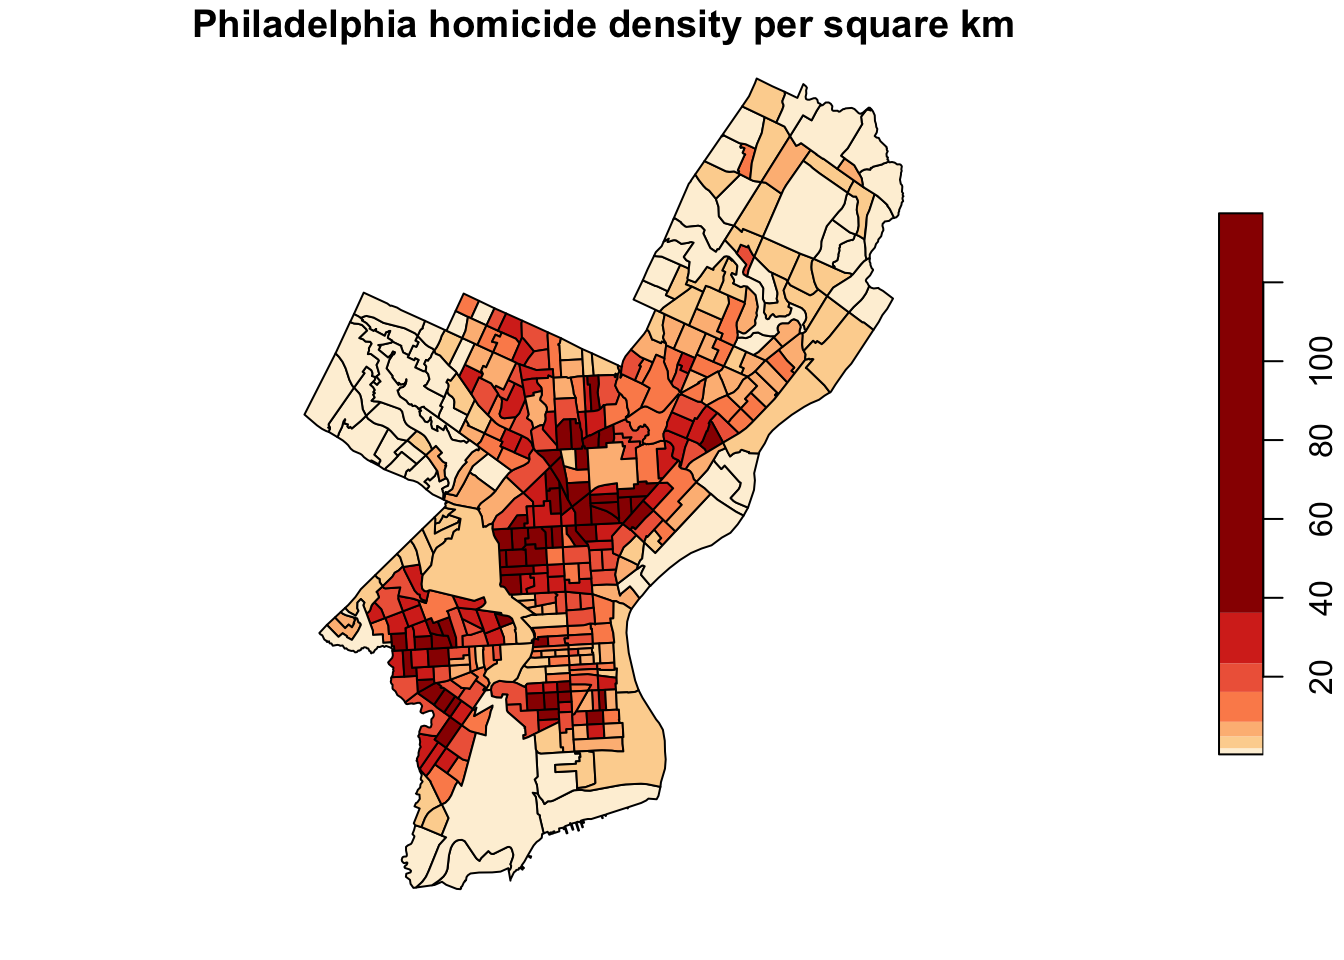
\includegraphics{R-spatial_files/figure-latex/sf-plot-legend-1.pdf}

\section{\texorpdfstring{Choropleth mapping with
\texttt{spplot}}{Choropleth mapping with spplot}}\label{choropleth-mapping-with-spplot}

\texttt{sp} comes with a plot command \texttt{spplot()}, which takes
\texttt{Spatial*} objects to plot. \texttt{spplot()} is one of the
earlier functions around to plot geographic objects.

\begin{Shaded}
\begin{Highlighting}[]
\NormalTok{philly_crimes_sp <-}\StringTok{ }\KeywordTok{readOGR}\NormalTok{(}\StringTok{"data/PhillyCrimerate/"}\NormalTok{, }\StringTok{"PhillyCrimerate"}\NormalTok{, }\DataTypeTok{verbose =} \OtherTok{FALSE}\NormalTok{) }\CommentTok{# verbose = FALSE omits the message on loading}
\KeywordTok{names}\NormalTok{(philly_crimes_sp)}
\end{Highlighting}
\end{Shaded}

\begin{verbatim}
#> [1] "GEOID10"    "n_homic"    "tract_area" "homic_rate"
\end{verbatim}

Like plot, by default \texttt{spplot} maps all everything it can find in
the attribute table. Sometimes this does not work, depending on the data
types in the attribute table. In order to select specific values to map
we can provide the \texttt{spplot} function with the name (or names) of
the attribute variable(s) we want to plot. It is the name of the column
of the \texttt{Spatial*Dataframe} as character string (or a vector if
several).

\begin{Shaded}
\begin{Highlighting}[]
\KeywordTok{spplot}\NormalTok{(philly_crimes_sp, }\StringTok{"homic_rate"}\NormalTok{)}
\end{Highlighting}
\end{Shaded}

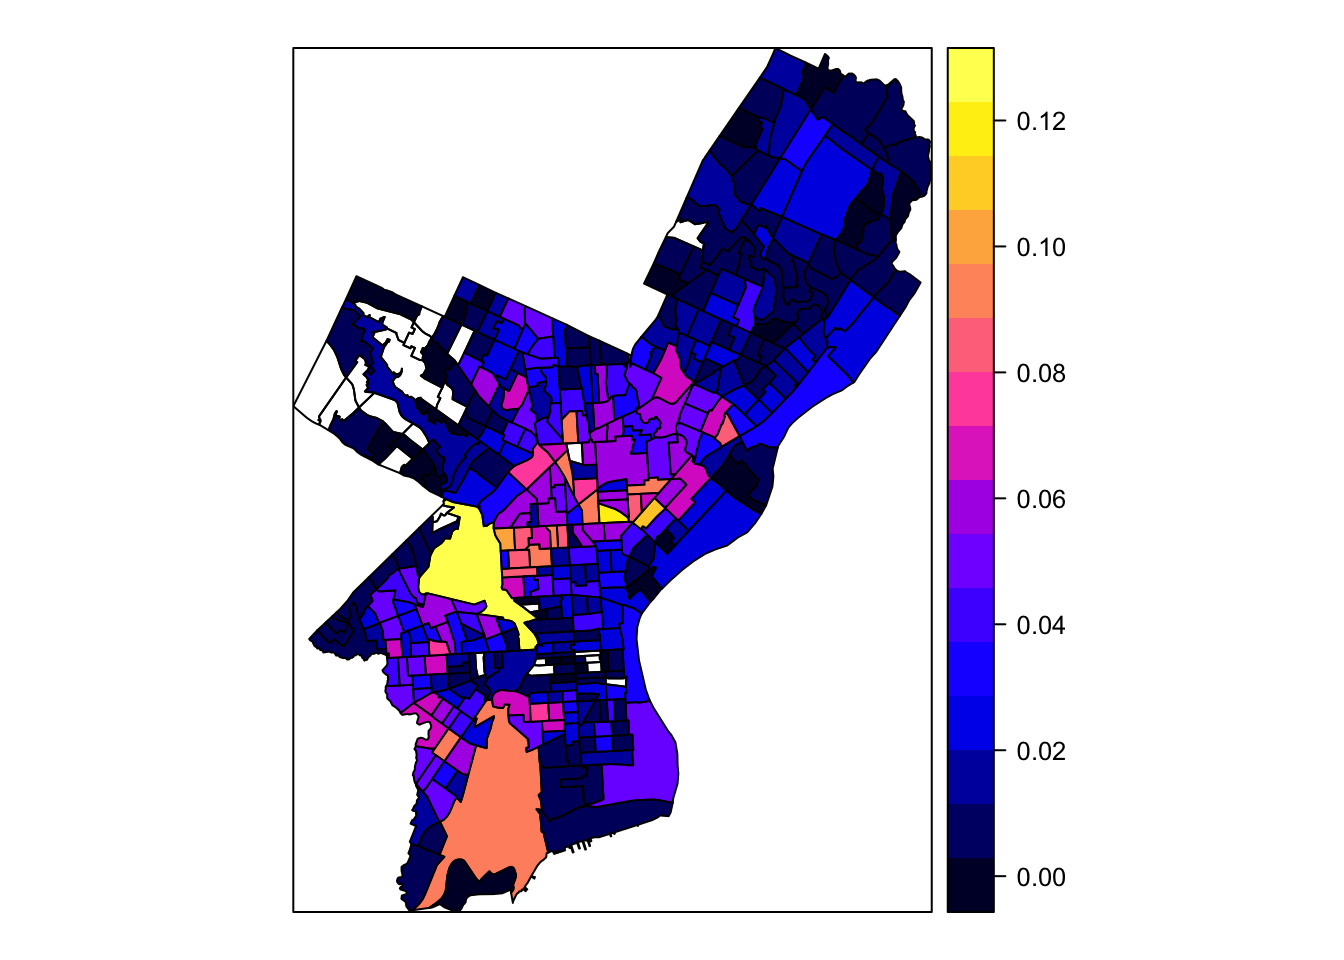
\includegraphics{R-spatial_files/figure-latex/spplot-single-1.pdf}

Many improvements can be made here as well, below is an
example\footnote{For more details see Chaps 2 and 3 in
  \href{https://asdar-book.org}{Applied Spatial Data Analysis with R}.
  Also, \texttt{spplot} is a wrapper for the
  \href{https://cran.r-project.org/package=lattice}{\texttt{lattice}
  package}, see there for more advanced options.} \footnote{For the
  correction of breaks after using classIntervals with spplot/levelplot
  see here
  \url{http://r.789695.n4.nabble.com/SpatialPolygon-with-the-max-value-gets-no-color-assigned-in-spplot-function-when-using-quot-at-quot-r-td4654672.html}}.

\begin{Shaded}
\begin{Highlighting}[]
\CommentTok{# quantile breaks}
\NormalTok{breaks_qt <-}\StringTok{ }\KeywordTok{classIntervals}\NormalTok{(philly_crimes_sp}\OperatorTok{$}\NormalTok{homic_rate, }\DataTypeTok{n =} \DecValTok{7}\NormalTok{, }\DataTypeTok{style =} \StringTok{"quantile"}\NormalTok{)}
\NormalTok{br <-}\StringTok{ }\NormalTok{breaks_qt}\OperatorTok{$}\NormalTok{brks }
\NormalTok{offs <-}\StringTok{ }\FloatTok{0.0000001} 
\NormalTok{br[}\DecValTok{1}\NormalTok{] <-}\StringTok{ }\NormalTok{br[}\DecValTok{1}\NormalTok{] }\OperatorTok{-}\StringTok{ }\NormalTok{offs }
\NormalTok{br[}\KeywordTok{length}\NormalTok{(br)] <-}\StringTok{ }\NormalTok{br[}\KeywordTok{length}\NormalTok{(br)] }\OperatorTok{+}\StringTok{ }\NormalTok{offs }
\CommentTok{# categoreis for choropleth map}
\NormalTok{philly_crimes_sp}\OperatorTok{$}\NormalTok{homic_rate_bracket <-}\StringTok{ }\KeywordTok{cut}\NormalTok{(philly_crimes_sp}\OperatorTok{$}\NormalTok{homic_rate, br)}
\CommentTok{# plot}
\KeywordTok{spplot}\NormalTok{(philly_crimes_sp, }\StringTok{"homic_rate_bracket"}\NormalTok{, }\DataTypeTok{col.regions=}\NormalTok{pal, }\DataTypeTok{main =} \StringTok{"Philadelphia homicide density per square km"}\NormalTok{)}
\end{Highlighting}
\end{Shaded}

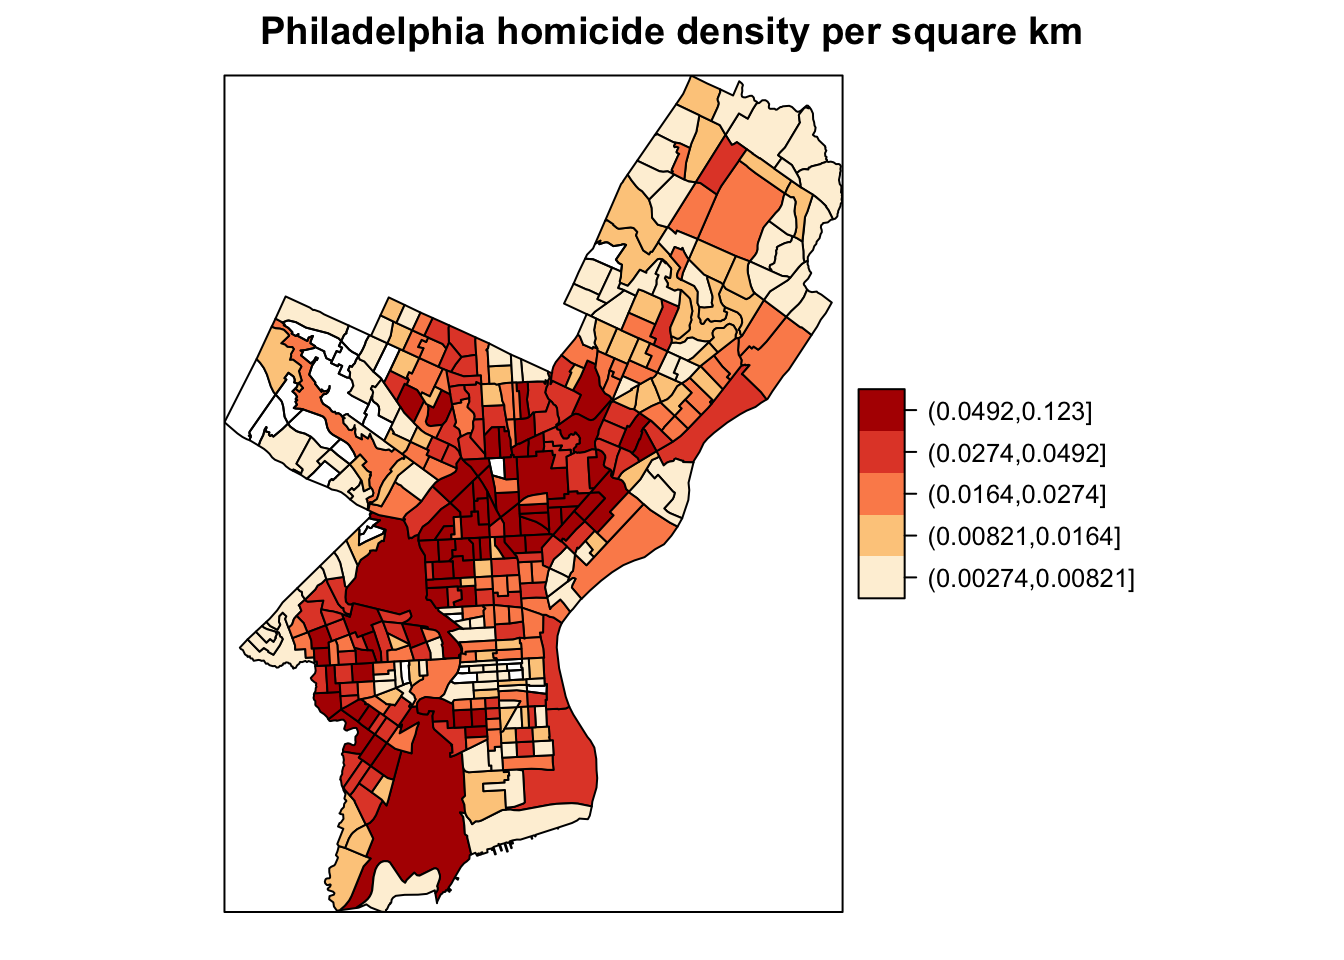
\includegraphics{R-spatial_files/figure-latex/spplot-final-map-1.pdf}

\section{\texorpdfstring{Choropleth mapping with
\texttt{ggplot2}}{Choropleth mapping with ggplot2}}\label{choropleth-mapping-with-ggplot2}

\href{http://ggplot2.org/}{\texttt{ggplot2}} is a widely used and
powerful plotting library for R. It is not specifically geared towards
mapping, but one can generate great maps.

The \texttt{ggplot()} syntax is different from the previous as a plot is
built up by adding components with a \texttt{+}. You can start with a
layer showing the raw data then add layers of annotations and
statistical summaries. This allows to easily superimpose either
different visualizations of one dataset (e.g.~a scatterplot and a fitted
line) or different datasets (like different layers of the same
geographical area)\footnote{See Wilkinson L (2005): ``The grammar of
  graphics''. Statistics and computing, 2nd ed. Springer, New York.}.

For an introduction to \texttt{ggplot} check out
\href{http://link.springer.com/book/10.1007\%2F978-3-319-24277-4}{this
book by the package creator} or
\href{http://ggplot2.tidyverse.org/}{this} for more pointers.

In order to build a plot you start with initializing a ggplot object. In
order to do that \texttt{ggplot()} takes:

\begin{itemize}
\tightlist
\item
  a data argument usually a \textbf{dataframe} and
\item
  a mapping argument where x and y values to be plotted are supplied.
\end{itemize}

In addition, minimally a geometry to be used to determine how the values
should be displayed. This is to be added after an \texttt{+}.

\begin{verbatim}
ggplot(data = my_data_frame, mapping = aes(x = name_of_column_with_x_value, y = name_of_column_with_y_value)) +
  geom_point()
\end{verbatim}

Or shorter:

\begin{verbatim}
ggplot(my_data_frame, aes(name_of_column_with_x_value, name_of_column_with_y_value)) +
  geom_point()
\end{verbatim}

The great news is that \textbf{\texttt{ggplot} can plot \texttt{sf}
objects directly} by using \texttt{geom\_sf}. So all we have to do is:

\begin{Shaded}
\begin{Highlighting}[]
\KeywordTok{ggplot}\NormalTok{(philly_crimes_sf) }\OperatorTok{+}\StringTok{ }
\StringTok{  }\KeywordTok{geom_sf}\NormalTok{(}\KeywordTok{aes}\NormalTok{(}\DataTypeTok{fill=}\NormalTok{homic_rate))}
\end{Highlighting}
\end{Shaded}

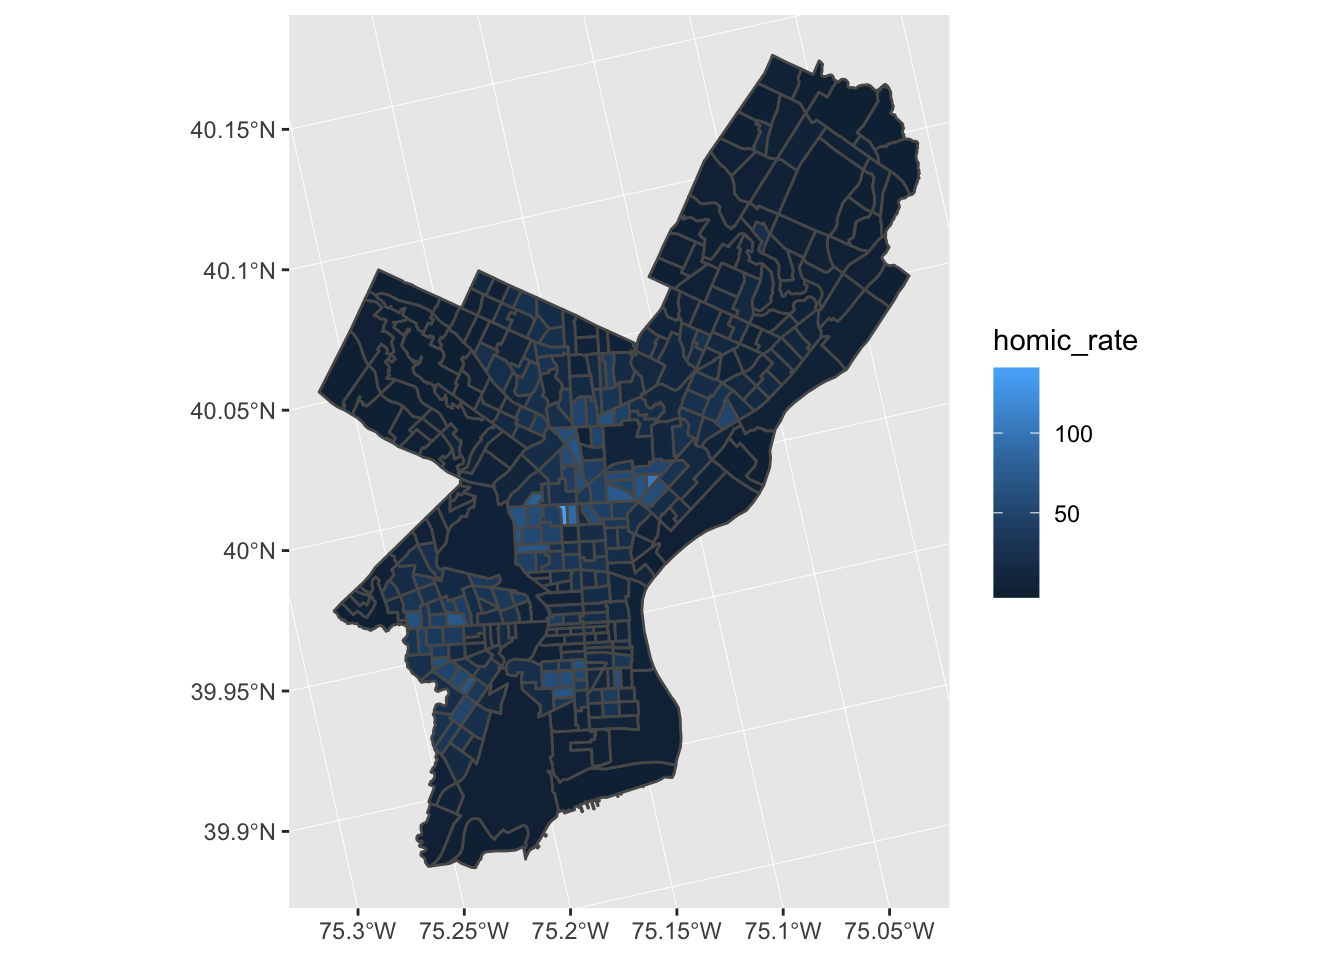
\includegraphics{R-spatial_files/figure-latex/ggplot-sf-1.pdf}

Homicide rate is a continuous variable and is plotted by \texttt{ggplot}
as such. If we wanted to plot our map as a `true' choropleth map we need
to convert our continouse variable into a categoriacal one, according to
whichever brackets we want to use.

This requires two steps:

\begin{itemize}
\tightlist
\item
  Determine the quantile breaks.
\item
  Add a categorical variable to the object which assigns each continious
  vaule to a bracket.
\end{itemize}

We will use the \texttt{classInt} package to explicitly determine the
breaks.

\begin{Shaded}
\begin{Highlighting}[]
\KeywordTok{library}\NormalTok{(classInt)}

\CommentTok{# get quantile breaks. Add .00001 offset to catch the lowest value}
\NormalTok{breaks_qt <-}\StringTok{ }\KeywordTok{classIntervals}\NormalTok{(}\KeywordTok{c}\NormalTok{(}\KeywordTok{min}\NormalTok{(philly_crimes_sf}\OperatorTok{$}\NormalTok{homic_rate) }\OperatorTok{-}\StringTok{ }\NormalTok{.}\DecValTok{00001}\NormalTok{, philly_crimes_sf}\OperatorTok{$}\NormalTok{homic_rate), }\DataTypeTok{n =} \DecValTok{7}\NormalTok{, }\DataTypeTok{style =} \StringTok{"quantile"}\NormalTok{)}

\NormalTok{breaks_qt}
\end{Highlighting}
\end{Shaded}

\begin{verbatim}
#> style: quantile
#> [0.2997339,1.856692)  [1.856692,4.814503)  [4.814503,8.495498) 
#>                   55                   55                   55 
#>  [8.495498,16.14234)  [16.14234,23.20642)  [23.20642,36.16089) 
#>                   55                   55                   55 
#>  [36.16089,137.5028] 
#>                   55
\end{verbatim}

Ok. We can retrieve the breaks with \texttt{breaks\$brks}.

We use \texttt{cut} to divice \texttt{homic\_rate} into intervals and
code them according to which interval they are in.

Lastly, we can use \texttt{scale\_fill\_brewer} and add our color
palette.

\begin{Shaded}
\begin{Highlighting}[]
\NormalTok{philly_crimes_sf <-}\StringTok{ }\KeywordTok{mutate}\NormalTok{(philly_crimes_sf, }\DataTypeTok{homic_rate_cat =} \KeywordTok{cut}\NormalTok{(homic_rate, breaks_qt}\OperatorTok{$}\NormalTok{brks)) }

\KeywordTok{ggplot}\NormalTok{(philly_crimes_sf) }\OperatorTok{+}\StringTok{ }
\StringTok{    }\KeywordTok{geom_sf}\NormalTok{(}\KeywordTok{aes}\NormalTok{(}\DataTypeTok{fill=}\NormalTok{homic_rate_cat)) }\OperatorTok{+}
\StringTok{    }\KeywordTok{scale_fill_brewer}\NormalTok{(}\DataTypeTok{palette =} \StringTok{"OrRd"}\NormalTok{) }
\end{Highlighting}
\end{Shaded}

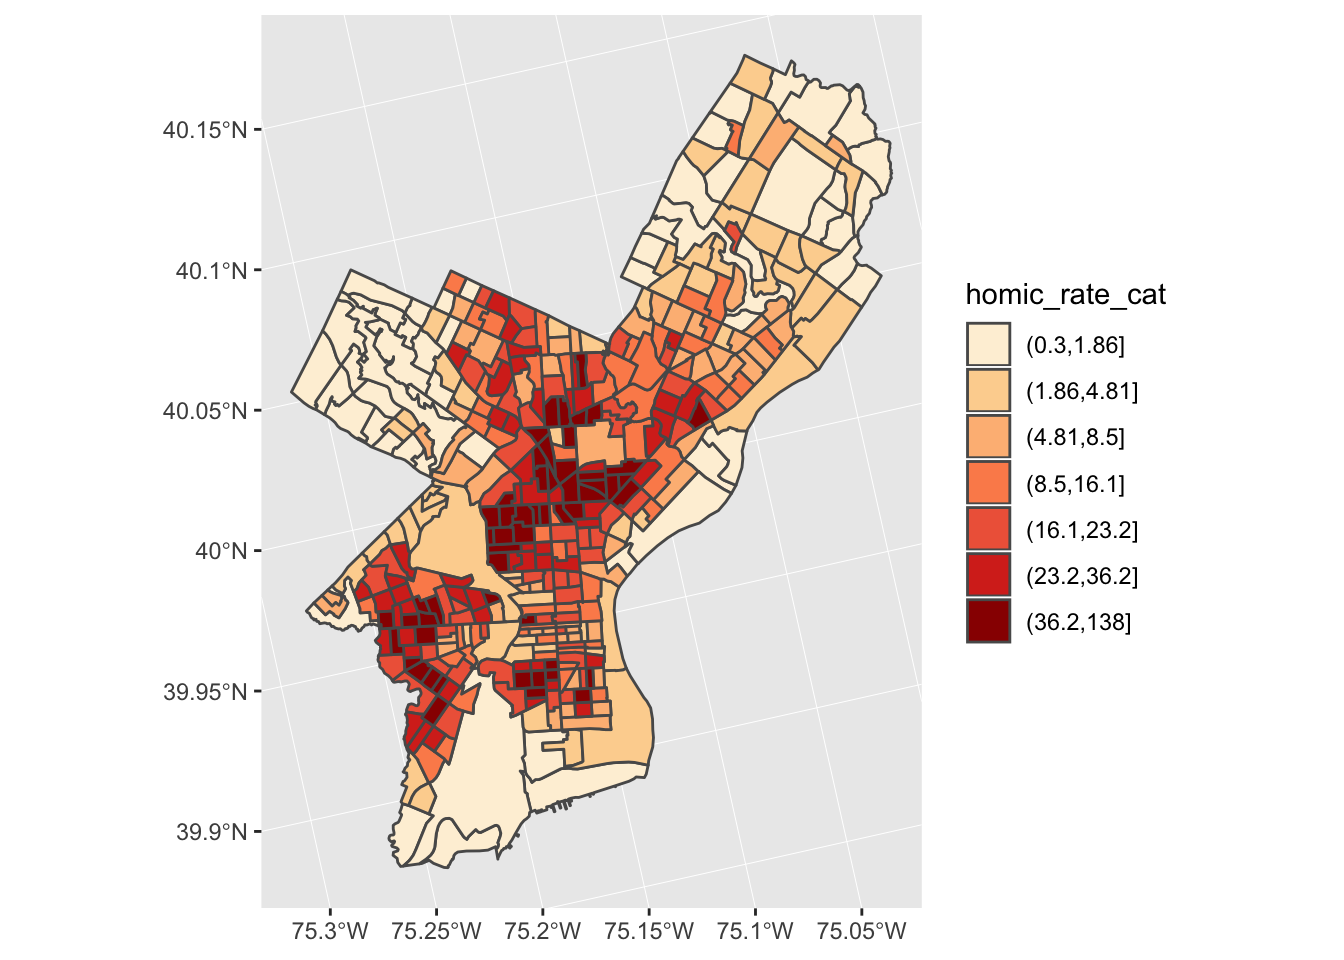
\includegraphics{R-spatial_files/figure-latex/ggplot-sf-categorical-1.pdf}

\section{\texorpdfstring{Adding basemaps with
\texttt{ggmap}}{Adding basemaps with ggmap}}\label{adding-basemaps-with-ggmap}

\texttt{ggmap} builds on \texttt{ggplot} and allows to pull in tiled
basemaps from different services, like Google Maps, OpenStreetMaps, or
Stamen Maps\footnote{Google now
  \href{https://cloud.google.com/maps-platform/.}{requires an API key}.
  Cloudmade maps retired its API so it is no longer possible to be used
  as basemap.
  \href{https://CRAN.R-project.org/package=RgoogleMaps}{\texttt{RgoogleMaps}}
  is another library that provides an interface to query the Google
  server for static maps.}.

So let's overlay the map from above on a terrain map we pull from
Stamen.

First we use the \texttt{get\_map()} command from \texttt{ggmap} to pull
down the basemap. We need to tell it the location or the boundaries of
the map, the zoom level, and what kind of map service we like (default
is Google terrain). It will actually download the tile.
\texttt{get\_map()} returns a ggmap object, name it
\texttt{ph\_basemap}. In order to view the map we then use
\texttt{ggmap()}.

\begin{Shaded}
\begin{Highlighting}[]
\KeywordTok{library}\NormalTok{(ggmap)}

\CommentTok{# Philadelphia Lat 39.95258 and Lon is -75.16522}
\NormalTok{ph_basemap <-}\StringTok{ }\KeywordTok{get_map}\NormalTok{(}\DataTypeTok{location=}\KeywordTok{c}\NormalTok{(}\DataTypeTok{lon =} \OperatorTok{-}\FloatTok{75.16522}\NormalTok{, }\DataTypeTok{lat =} \FloatTok{39.95258}\NormalTok{), }\DataTypeTok{zoom=}\DecValTok{11}\NormalTok{, }\DataTypeTok{maptype =} \StringTok{'terrain-background'}\NormalTok{, }\DataTypeTok{source =} \StringTok{'stamen'}\NormalTok{)}

\KeywordTok{ggmap}\NormalTok{(ph_basemap)}
\end{Highlighting}
\end{Shaded}

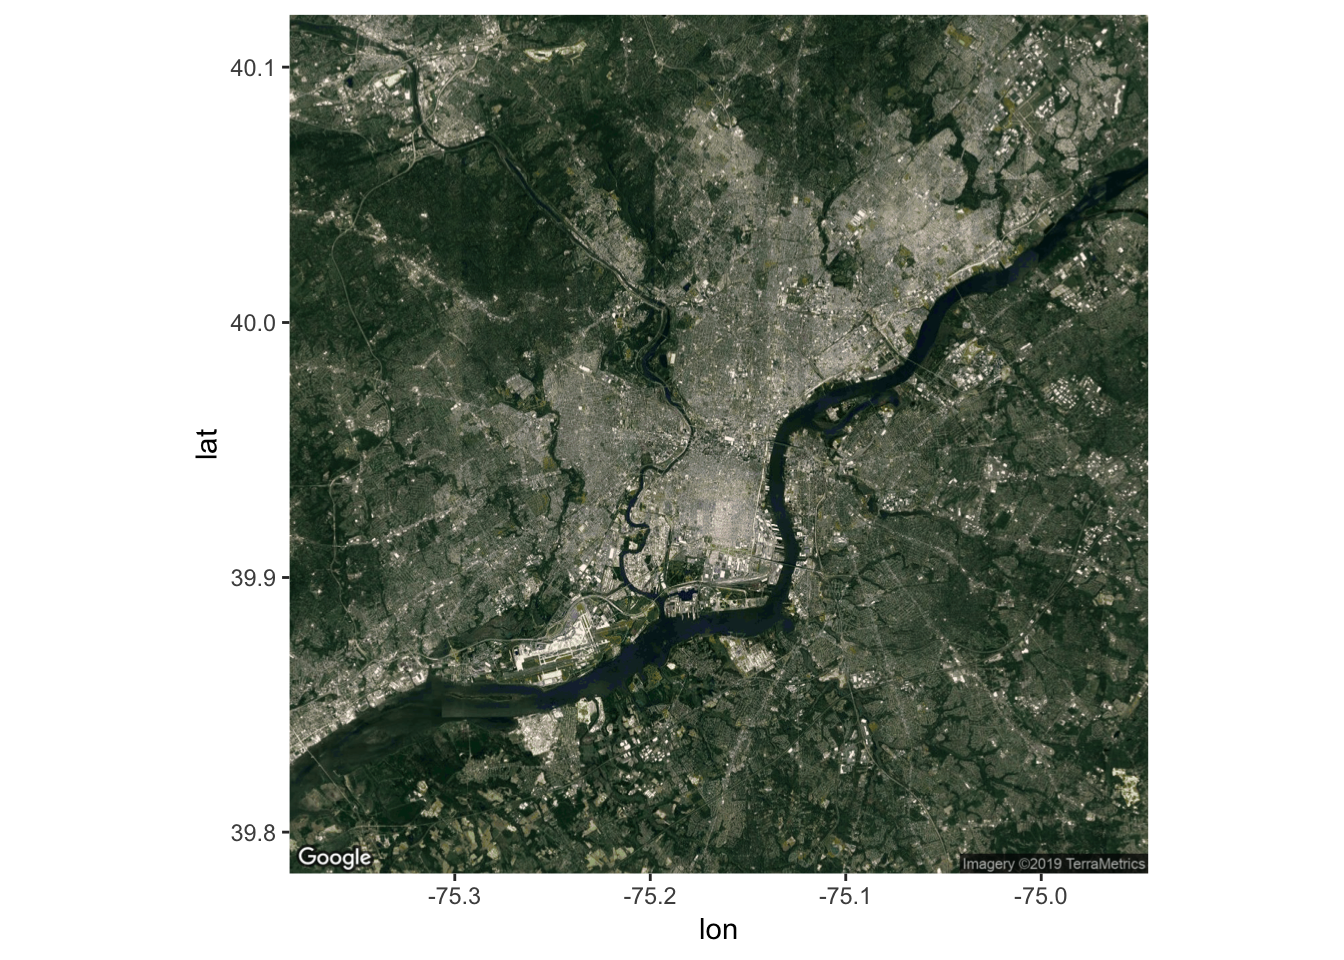
\includegraphics{R-spatial_files/figure-latex/ggmap-getmap-1.pdf}

Then we can reuse the code from the ggplot example above, just replacing
the first line, where we initialized a ggplot object above

\begin{verbatim}
    ggplot() + 
\end{verbatim}

with the line to call our basemap:

\begin{verbatim}
    ggmap(ph_basemap) +
\end{verbatim}

We also have to set \texttt{inherit.aes} to \texttt{FALSE}, so it
overrides the default aesthetics (from the ggmap object).

\begin{Shaded}
\begin{Highlighting}[]
\KeywordTok{ggmap}\NormalTok{(ph_basemap) }\OperatorTok{+}
\StringTok{    }\KeywordTok{geom_sf}\NormalTok{(}\DataTypeTok{data =}\NormalTok{ philly_crimes_sf, }\KeywordTok{aes}\NormalTok{(}\DataTypeTok{fill=}\NormalTok{homic_rate_cat), }\DataTypeTok{inherit.aes =} \OtherTok{FALSE}\NormalTok{) }\OperatorTok{+}
\StringTok{    }\KeywordTok{scale_fill_brewer}\NormalTok{(}\DataTypeTok{palette =} \StringTok{"OrRd"}\NormalTok{)}
\end{Highlighting}
\end{Shaded}

\begin{verbatim}
#> Coordinate system already present. Adding new coordinate system, which will replace the existing one.
\end{verbatim}

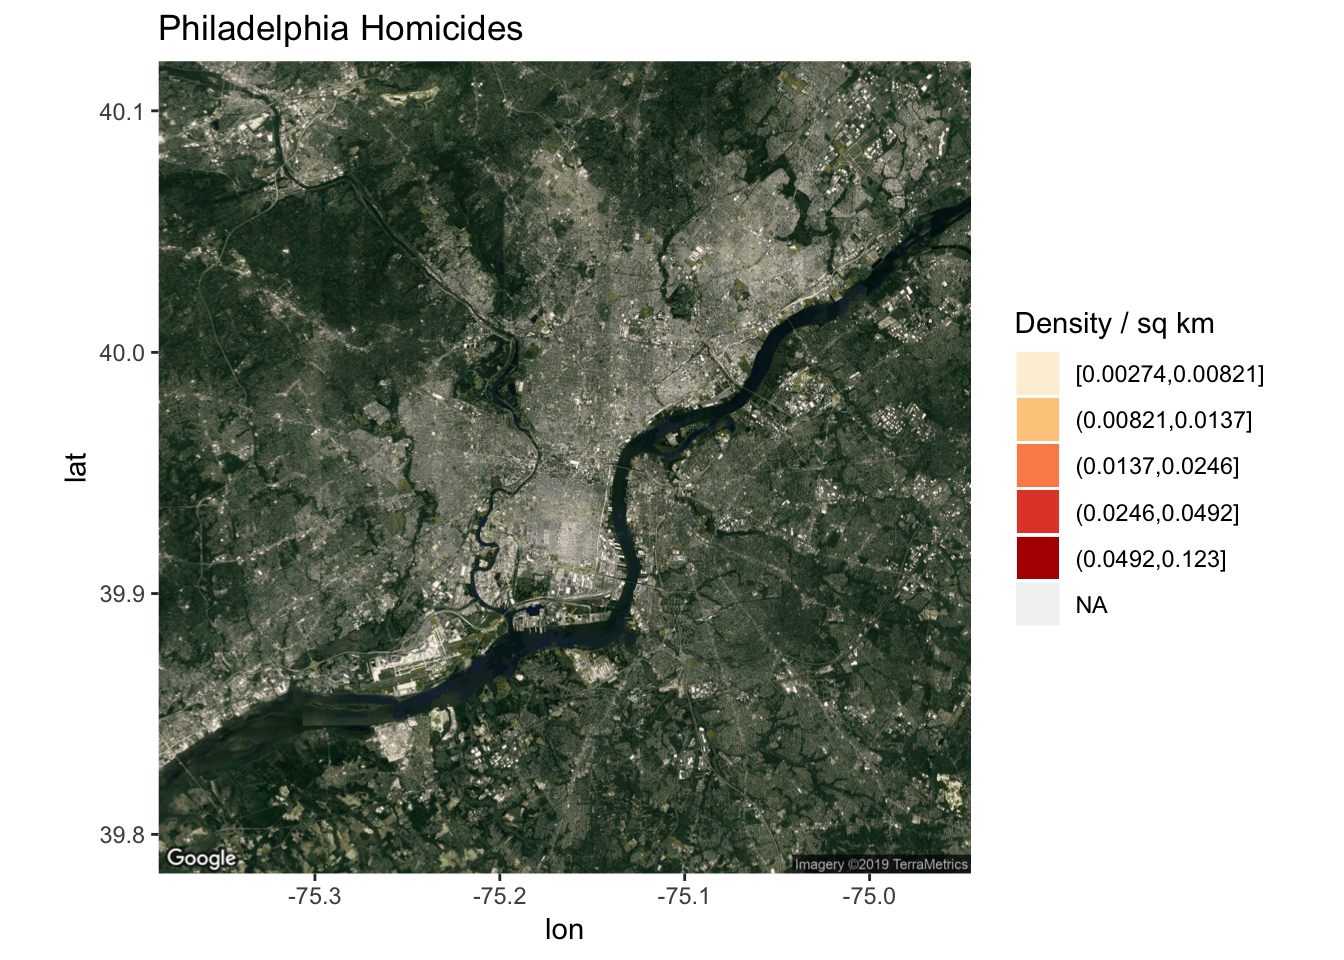
\includegraphics{R-spatial_files/figure-latex/ggmap-plot-misaligned-1.pdf}

Oops. Any idea what might be going on?

We need to set our CRS to WGS84, which is the one the tiles are
downloaded in. We can add \texttt{coord\_sf} to do this:

\begin{Shaded}
\begin{Highlighting}[]
\KeywordTok{ggmap}\NormalTok{(ph_basemap) }\OperatorTok{+}
\StringTok{    }\KeywordTok{geom_sf}\NormalTok{(}\DataTypeTok{data =}\NormalTok{ philly_crimes_sf, }\KeywordTok{aes}\NormalTok{(}\DataTypeTok{fill=}\NormalTok{homic_rate_cat), }\DataTypeTok{inherit.aes =} \OtherTok{FALSE}\NormalTok{) }\OperatorTok{+}
\StringTok{    }\KeywordTok{scale_fill_brewer}\NormalTok{(}\DataTypeTok{palette =} \StringTok{"OrRd"}\NormalTok{) }\OperatorTok{+}
\StringTok{    }\KeywordTok{coord_sf}\NormalTok{(}\DataTypeTok{crs =} \KeywordTok{st_crs}\NormalTok{(}\DecValTok{4326}\NormalTok{))}
\end{Highlighting}
\end{Shaded}

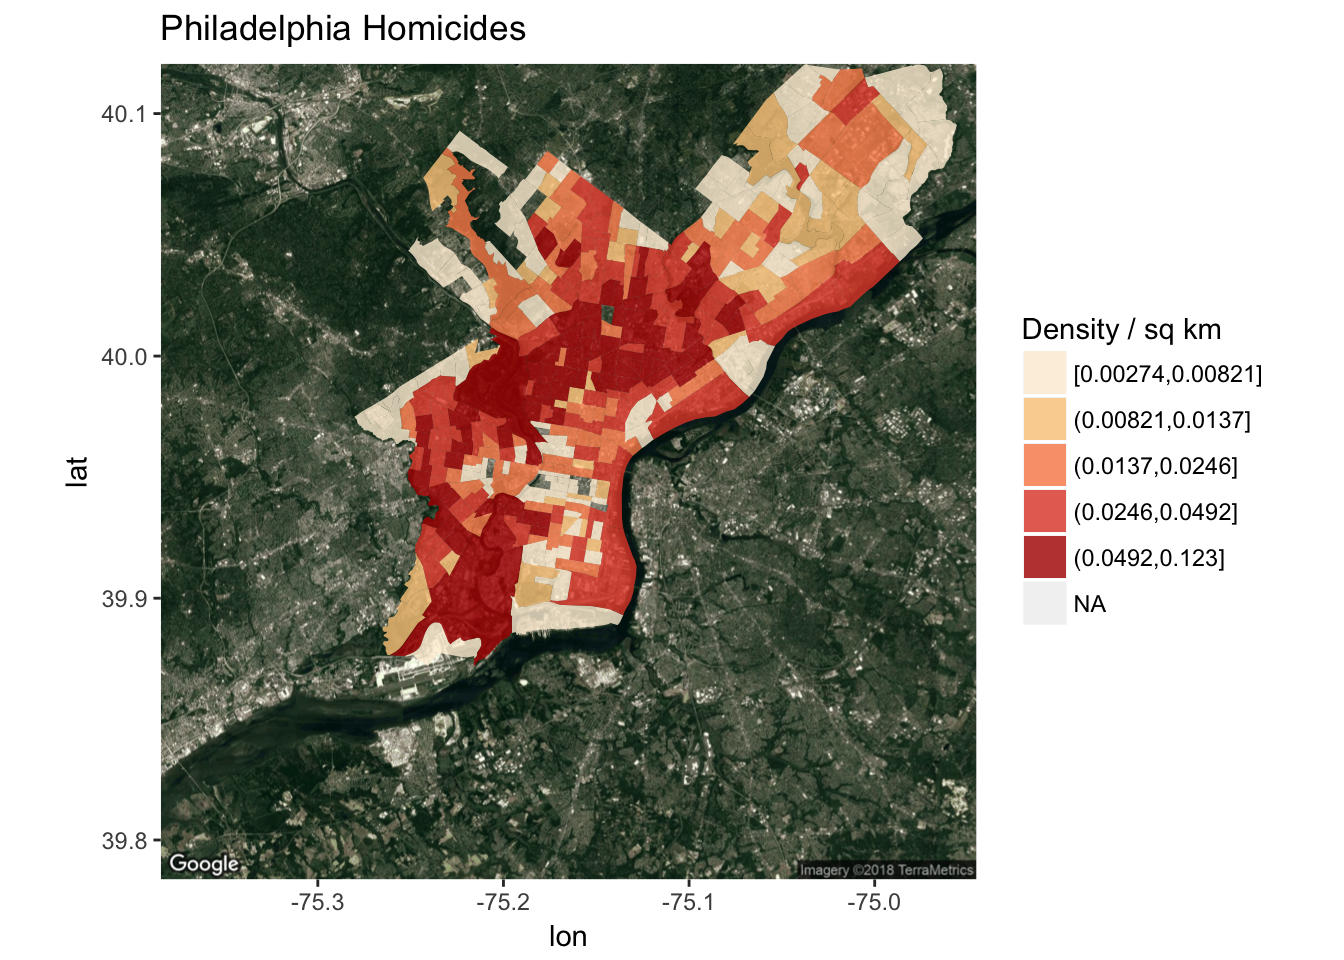
\includegraphics{R-spatial_files/figure-latex/ggmap-plot-aligned-1.pdf}

The \texttt{ggmap} package also includes functions for distance
calculations, geocoding, and calculating routes.

\section{\texorpdfstring{Choropleth with
\texttt{tmap}}{Choropleth with tmap}}\label{choropleth-with-tmap}

\texttt{tmap} is specifically designed to make creation of thematic maps
more convenient. It borrows from teh ggplot syntax and takes care of a
lot of the styling and aesthetics. This reduces our amount of code
significantly. We only need:

\begin{itemize}
\tightlist
\item
  \texttt{tm\_shape()} where we provide

  \begin{itemize}
  \tightlist
  \item
    the \texttt{sf} object (we could also provide an
    \texttt{SpatialPolygonsDataframe})
  \end{itemize}
\item
  \texttt{tm\_polygons()} where we set

  \begin{itemize}
  \tightlist
  \item
    the attribute variable to map,
  \item
    the break style, and
  \item
    a title.
  \end{itemize}
\end{itemize}

\begin{Shaded}
\begin{Highlighting}[]
\KeywordTok{library}\NormalTok{(tmap)}
\KeywordTok{tm_shape}\NormalTok{(philly_crimes_sf) }\OperatorTok{+}
\StringTok{  }\KeywordTok{tm_polygons}\NormalTok{(}\StringTok{"homic_rate"}\NormalTok{, }
              \DataTypeTok{style=}\StringTok{"quantile"}\NormalTok{, }
              \DataTypeTok{title=}\StringTok{"Philadelphia }\CharTok{\textbackslash{}n}\StringTok{homicide density }\CharTok{\textbackslash{}n}\StringTok{per sqKm"}\NormalTok{)}
\end{Highlighting}
\end{Shaded}

\begin{verbatim}
#> PhantomJS not found. You can install it with webshot::install_phantomjs(). If it is installed, please make sure the phantomjs executable can be found via the PATH variable.
\end{verbatim}

\hypertarget{htmlwidget-5f5f8684d951cb546c80}{}

\texttt{tmap} has a very nice feature that allows us to give basic
interactivity to the map. We can switch from ``plot'' mode into ``view''
mode and call the last plot, like so:

\begin{Shaded}
\begin{Highlighting}[]
\KeywordTok{tmap_mode}\NormalTok{(}\StringTok{"view"}\NormalTok{)}
\KeywordTok{tmap_last}\NormalTok{()}
\end{Highlighting}
\end{Shaded}

\hypertarget{htmlwidget-bb462369a55246093d7c}{}

Cool huh?

The \texttt{tmap} library also includes functions for simple spatial
operations, geocoding and reverse geocoding using OSM. For more check
\texttt{vignette("tmap-getstarted")}.

\section{\texorpdfstring{Web mapping with
\texttt{leaflet}}{Web mapping with leaflet}}\label{web-mapping-with-leaflet}

\texttt{leaflet} provides bindings to the
\href{http://leafletjs.com}{`Leaflet' JavaScript library}, ``the leading
open-source JavaScript library for mobile-friendly interactive maps''.
We have already seen a simple use of leaflet in the \texttt{tmap}
example.

The good news is that the \texttt{leaflet} library gives us loads of
options to customize the web look and feel of the map.

The bad news is that the \texttt{leaflet} library gives us loads of
options to customize the web look and feel of the map.

Let's build up the map step by step.

First we load the \texttt{leaflet} library. Use the \texttt{leaflet()}
function with an \texttt{sp} or \texttt{Spatial*} object and pipe it to
\texttt{addPolygons()} function. It is not required, but improves
readability if you use \href{https://github.com/tidyverse/magrittr}{the
pipe operator \texttt{\%\textgreater{}\%}} to chain the elements
together when building up a map with \texttt{leaflet}.

And while \texttt{tmap} was tolerant about our AEA projection of
\texttt{philly\_crimes\_sf}, \texttt{leaflet} does require us to
explicitly reproject the \texttt{sf} object.

\begin{Shaded}
\begin{Highlighting}[]
\KeywordTok{library}\NormalTok{(leaflet) }

\CommentTok{# reproject}
\NormalTok{philly_WGS84 <-}\StringTok{ }\KeywordTok{st_transform}\NormalTok{(philly_crimes_sf, }\DecValTok{4326}\NormalTok{)}

\KeywordTok{leaflet}\NormalTok{(philly_WGS84) }\OperatorTok
\StringTok{  }\KeywordTok{addPolygons}\NormalTok{()}
\end{Highlighting}
\end{Shaded}

\hypertarget{htmlwidget-efe98f31523f93920651}{}

To map the homicide density we use \texttt{addPolygons()} and:

\begin{itemize}
\tightlist
\item
  remove stroke (polygon borders)\\
\item
  set a fillColor for each polygon based on \texttt{homic\_rate} and
  make it look nice by adjusting fillOpacity and smoothFactor (how much
  to simplify the polyline on each zoom level). The fill color is
  generated using \texttt{leaflet}'s \texttt{colorQuantile()} function,
  which takes the color scheme and the desired number of classes. To
  constuct the color scheme \texttt{colorQuantile()} returns a function
  that we supply to \texttt{addPolygons()} together with the name of the
  attribute variable to map.\\
\item
  add a popup with the \texttt{homic\_rate} values. We will create as a
  vector of strings, that we then supply to \texttt{addPolygons()}.
\end{itemize}

\begin{Shaded}
\begin{Highlighting}[]
\NormalTok{pal_fun <-}\StringTok{ }\KeywordTok{colorQuantile}\NormalTok{(}\StringTok{"YlOrRd"}\NormalTok{, }\OtherTok{NULL}\NormalTok{, }\DataTypeTok{n =} \DecValTok{5}\NormalTok{)}

\NormalTok{p_popup <-}\StringTok{ }\KeywordTok{paste0}\NormalTok{(}\StringTok{"<strong>Homicide Density: </strong>"}\NormalTok{, philly_WGS84}\OperatorTok{$}\NormalTok{homic_rate)}

\KeywordTok{leaflet}\NormalTok{(philly_WGS84) }\OperatorTok
\StringTok{  }\KeywordTok{addPolygons}\NormalTok{(}
    \DataTypeTok{stroke =} \OtherTok{FALSE}\NormalTok{, }\CommentTok{# remove polygon borders}
    \DataTypeTok{fillColor =} \OperatorTok{~}\KeywordTok{pal_fun}\NormalTok{(homic_rate), }\CommentTok{# set fill color with function from above and value}
    \DataTypeTok{fillOpacity =} \FloatTok{0.8}\NormalTok{, }\DataTypeTok{smoothFactor =} \FloatTok{0.5}\NormalTok{, }\CommentTok{# make it nicer}
    \DataTypeTok{popup =}\NormalTok{ p_popup)  }\CommentTok{# add popup}
\end{Highlighting}
\end{Shaded}

\hypertarget{htmlwidget-326bbb586065c8d62175}{}

Here we add a basemap, which defaults to OSM, with \texttt{addTiles()}

\begin{Shaded}
\begin{Highlighting}[]
\KeywordTok{leaflet}\NormalTok{(philly_WGS84) }\OperatorTok
\StringTok{  }\KeywordTok{addPolygons}\NormalTok{(}
    \DataTypeTok{stroke =} \OtherTok{FALSE}\NormalTok{, }
    \DataTypeTok{fillColor =} \OperatorTok{~}\KeywordTok{pal_fun}\NormalTok{(homic_rate),}
    \DataTypeTok{fillOpacity =} \FloatTok{0.8}\NormalTok{, }\DataTypeTok{smoothFactor =} \FloatTok{0.5}\NormalTok{,}
    \DataTypeTok{popup =}\NormalTok{ p_popup) }\OperatorTok
\StringTok{  }\KeywordTok{addTiles}\NormalTok{()}
\end{Highlighting}
\end{Shaded}

\hypertarget{htmlwidget-bb2179248924f8cd92ed}{}

Lastly, we add a legend. We will provide the \texttt{addLegend()}
function with:

\begin{itemize}
\tightlist
\item
  the location of the legend on the map\\
\item
  the function that creates the color palette\\
\item
  the value we want the palette function to use\\
\item
  a title
\end{itemize}

\begin{Shaded}
\begin{Highlighting}[]
\KeywordTok{leaflet}\NormalTok{(philly_WGS84) }\OperatorTok
\StringTok{  }\KeywordTok{addPolygons}\NormalTok{(}
    \DataTypeTok{stroke =} \OtherTok{FALSE}\NormalTok{, }
    \DataTypeTok{fillColor =} \OperatorTok{~}\KeywordTok{pal_fun}\NormalTok{(homic_rate),}
    \DataTypeTok{fillOpacity =} \FloatTok{0.8}\NormalTok{, }\DataTypeTok{smoothFactor =} \FloatTok{0.5}\NormalTok{,}
    \DataTypeTok{popup =}\NormalTok{ p_popup) }\OperatorTok
\StringTok{  }\KeywordTok{addTiles}\NormalTok{() }\OperatorTok
\StringTok{  }\KeywordTok{addLegend}\NormalTok{(}\StringTok{"bottomright"}\NormalTok{,  }\CommentTok{# location}
            \DataTypeTok{pal=}\NormalTok{pal_fun,    }\CommentTok{# palette function}
            \DataTypeTok{values=}\OperatorTok{~}\NormalTok{homic_rate,  }\CommentTok{# value to be passed to palette function}
            \DataTypeTok{title =} \StringTok{'Philadelphia homicide density per sqkm'}\NormalTok{) }\CommentTok{# legend title}
\end{Highlighting}
\end{Shaded}

\hypertarget{htmlwidget-98d9098218d1aa7f6f9b}{}

The labels of the legend show percentages instead of the actual value
breaks\footnote{The formatting is set with \texttt{labFormat()} and in
  the
  \href{https://cran.r-project.org/web/packages/leaflet/leaflet.pdf}{documentation}
  we discover that: ``By default, \texttt{labFormat} is basically
  \texttt{format(scientific\ =\ FALSE,big.mark\ =\ \textquotesingle{},\textquotesingle{})}
  for the numeric palette, \texttt{as.character()} for the factor
  palette, and a function to return labels of the form
  \texttt{x{[}i{]}\ -\ x{[}i\ +\ 1{]}} for bin and quantile palettes
  (\textbf{in the case of quantile palettes, x is the probabilities
  instead of the values of breaks}).''}.

To set the labels for our breaks manually we replace the \texttt{pal}
and \texttt{values} with the \texttt{colors} and \texttt{labels}
arguments and set those directly using \texttt{brewer.pal()} and
\texttt{breaks\_qt} from an earlier section above.

\begin{Shaded}
\begin{Highlighting}[]
\KeywordTok{leaflet}\NormalTok{(philly_WGS84) }\OperatorTok
\StringTok{  }\KeywordTok{addPolygons}\NormalTok{(}
    \DataTypeTok{stroke =} \OtherTok{FALSE}\NormalTok{, }
    \DataTypeTok{fillColor =} \OperatorTok{~}\KeywordTok{pal_fun}\NormalTok{(homic_rate),}
    \DataTypeTok{fillOpacity =} \FloatTok{0.8}\NormalTok{, }\DataTypeTok{smoothFactor =} \FloatTok{0.5}\NormalTok{,}
    \DataTypeTok{popup =}\NormalTok{ p_popup) }\OperatorTok
\StringTok{  }\KeywordTok{addTiles}\NormalTok{() }\OperatorTok
\StringTok{  }\KeywordTok{addLegend}\NormalTok{(}\StringTok{"bottomright"}\NormalTok{, }
            \DataTypeTok{colors =} \KeywordTok{brewer.pal}\NormalTok{(}\DecValTok{7}\NormalTok{, }\StringTok{"YlOrRd"}\NormalTok{), }
            \DataTypeTok{labels =} \KeywordTok{paste0}\NormalTok{(}\StringTok{"up to "}\NormalTok{, }\KeywordTok{format}\NormalTok{(breaks_qt}\OperatorTok{$}\NormalTok{brks[}\OperatorTok{-}\DecValTok{1}\NormalTok{], }\DataTypeTok{digits =} \DecValTok{2}\NormalTok{)),}
            \DataTypeTok{title =}  \StringTok{'Philadelphia homicide density per sqkm'}\NormalTok{)}
\end{Highlighting}
\end{Shaded}

\hypertarget{htmlwidget-5be8ceb733a66c2ac986}{}

That's more like it. Finally, I have added for you a control to switch
to another basemap and turn the philly polygon off and on. Take a look
at the changes in the code below.

\begin{Shaded}
\begin{Highlighting}[]
\KeywordTok{leaflet}\NormalTok{(philly_WGS84) }\OperatorTok
\StringTok{  }\KeywordTok{addPolygons}\NormalTok{(}
    \DataTypeTok{stroke =} \OtherTok{FALSE}\NormalTok{, }
    \DataTypeTok{fillColor =} \OperatorTok{~}\KeywordTok{pal_fun}\NormalTok{(homic_rate),}
    \DataTypeTok{fillOpacity =} \FloatTok{0.8}\NormalTok{, }\DataTypeTok{smoothFactor =} \FloatTok{0.5}\NormalTok{,}
    \DataTypeTok{popup =}\NormalTok{ p_popup,}
    \DataTypeTok{group =} \StringTok{"philly"}\NormalTok{) }\OperatorTok
\StringTok{  }\KeywordTok{addTiles}\NormalTok{(}\DataTypeTok{group =} \StringTok{"OSM"}\NormalTok{) }\OperatorTok
\StringTok{  }\KeywordTok{addProviderTiles}\NormalTok{(}\StringTok{"CartoDB.DarkMatter"}\NormalTok{, }\DataTypeTok{group =} \StringTok{"Carto"}\NormalTok{) }\OperatorTok
\StringTok{  }\KeywordTok{addLegend}\NormalTok{(}\StringTok{"bottomright"}\NormalTok{, }
            \DataTypeTok{colors =} \KeywordTok{brewer.pal}\NormalTok{(}\DecValTok{7}\NormalTok{, }\StringTok{"YlOrRd"}\NormalTok{), }
            \DataTypeTok{labels =} \KeywordTok{paste0}\NormalTok{(}\StringTok{"up to "}\NormalTok{, }\KeywordTok{format}\NormalTok{(breaks_qt}\OperatorTok{$}\NormalTok{brks[}\OperatorTok{-}\DecValTok{1}\NormalTok{], }\DataTypeTok{digits =} \DecValTok{2}\NormalTok{)),}
            \DataTypeTok{title =} \StringTok{'Philadelphia homicide density per sqkm'}\NormalTok{) }\OperatorTok
\StringTok{  }\KeywordTok{addLayersControl}\NormalTok{(}\DataTypeTok{baseGroups =} \KeywordTok{c}\NormalTok{(}\StringTok{"OSM"}\NormalTok{, }\StringTok{"Carto"}\NormalTok{), }
                   \DataTypeTok{overlayGroups =} \KeywordTok{c}\NormalTok{(}\StringTok{"philly"}\NormalTok{))  }
\end{Highlighting}
\end{Shaded}

\hypertarget{htmlwidget-3b43a8bbf2d6b0bb95c2}{}

If you'd like to take this further here are a few pointers.

\begin{itemize}
\tightlist
\item
  \href{http://rstudio.github.io/leaflet/}{Leaflet for R}
\item
  \href{https://github.com/Robinlovelace/Creating-maps-in-R/blob/master/vignettes/vspd-base-shiny.Rmd}{Creating
  maps in R}
\item
  \href{https://cyberhelp.sesync.org/maps-in-R-lesson/}{Maps in R}
\end{itemize}

\href{https://cengel.shinyapps.io/RioSlaveMarket/}{Here is an example}
using \texttt{ggplot}, \texttt{leaflet}, \texttt{shiny}, and
\href{http://rmarkdown.rstudio.com/flexdashboard/}{RStudio's
flexdashboard} template to bring it all together.

\bibliography{book.bib,packages.bib}


\end{document}
